\documentclass[11pt,openany]{book}
\usepackage[utf8]{inputenc}
\usepackage[T1]{fontenc}
\usepackage[dvips,a4paper,hmargin={3cm,3cm},vmargin={2cm,2cm}]{geometry}
\usepackage[a4paper,colorlinks=true,bookmarksopen=false,linkcolor=brown,citecolor=red]{hyperref}
\usepackage{tikz}
\usepackage{datetime2} 
\usepackage{pythontex}
\usepackage{calc}
\usepackage{comment}
\usepackage{amssymb}
\usepackage{amsthm}
\usepackage{amsmath}
\usepackage{amsrefs}
\usepackage{thmtools}
\usepackage{titlesec}
\usepackage{titletoc}
\usepackage{dsfont}
\usepackage{euscript}
\usepackage{fourier-orns}
\usepackage{fontawesome}
% \usepackage{mathpazo}
\usepackage{graphicx}
\usepackage[framemethod=TikZ]{mdframed}
\usepackage{tikz-cd}
\tikzcdset{
arrow style=tikz,
diagrams={>=latex}
}

\def\RR{\mathds R}
\def\ZZ{\mathds Z}
\def\NN{\mathds N}
\def\QQ{\mathds Q}
\def\P{\EuScript P}
\def\0{\varnothing}
\def\E{{\rm E}}
\def\Var{{\rm Var}}
\def\coVar{{\rm co\kern-0.3ex Var}}
\def\range{\mathop{\rm img}}
\linespread{1.2}
\setlength{\parindent}{0ex}
\setlength{\parskip}{.5\baselineskip}

% \DeclareFontFamily{OT1}{pzc}{}
% \DeclareFontShape{OT1}{pzc}{m}{it}{<-> s * [1.10] pzcmi7t}{}
% \DeclareMathAlphabet{\mathpzc}{OT1}{pzc}{m}{it} 


\newcommand{\mylabel}[1]{{\footnotesize\textsf{#1}}\hfill}
\renewenvironment{itemize}
  {\begin{list}{$\triangleright$}{%
   \setlength{\parskip}{0mm}
   \setlength{\topsep}{.2\baselineskip}
   \setlength{\rightmargin}{0mm}
   \setlength{\listparindent}{0mm}
   \setlength{\itemindent}{0mm}
   \setlength{\labelwidth}{3ex}
   \setlength{\itemsep}{.4\baselineskip}
   \setlength{\parsep}{0mm}
   \setlength{\partopsep}{0mm}
   \setlength{\labelsep}{1ex}
   \setlength{\leftmargin}{\labelwidth+\labelsep}
   \let\makelabel\mylabel}}{%
   \end{list}\vspace*{-1.3mm}}

   
\newenvironment{citemize}
  {\begin{list}{$\triangleright$}{%
   \setlength{\parskip}{0mm}
   \setlength{\topsep}{.2\baselineskip}
   \setlength{\rightmargin}{0mm}
   \setlength{\listparindent}{0mm}
   \setlength{\itemindent}{0mm}
   \setlength{\labelwidth}{3ex}
   \setlength{\itemsep}{.1\baselineskip}
   \setlength{\parsep}{0mm}
   \setlength{\partopsep}{0mm}
   \setlength{\labelsep}{1ex}
   \setlength{\leftmargin}{\labelwidth+\labelsep}
   \let\makelabel\mylabel}}{%
   \end{list}\vspace*{-1.3mm}}

\definecolor{blue}{rgb}{0, 0.1, 0.6}
\def\emph#1{\textcolor{blue}{\textbf{\boldmath #1}}}

\def\theta{\vartheta}
\def\phi{\varphi}
\def\epsilon{\varepsilon}
\def\ssf#1{\textsf{\small #1}}


\titleformat
{\chapter} % command
[display] % shape
{\bfseries\LARGE} % format
{Chapter \ \thechapter} % label
{0.5ex} % sep
{} % before-code
[] % after-code
\titleformat{\section}[block]{\large\bfseries}{\makebox[5ex][r]{\textbf{\thesection}}}{1.5ex}{}
\titlespacing{\subsection}{0ex}{.5ex plus .5ex minus .5ex}{1ex plus .2ex minus .2ex}
\titlespacing*{\chapter}{0em}{.5ex plus .2ex minus .2ex}{2.3ex plus .2ex}
\titlespacing*{\section}{-9.7ex}{3ex plus .5ex minus .5ex}{1ex plus .2ex minus .2ex}

\renewcommand*\thesection{\arabic{section}}

% \newcommand{\mylabel}[1]{{#1}\hfill}
% \renewenvironment{itemize}
%   {\begin{list}{$\cdot$}{%
%   \setlength{\parskip}{0mm}
%   \setlength{\topsep}{.2\baselineskip}
%   \setlength{\rightmargin}{0mm}
%   \setlength{\listparindent}{0mm}
%   \setlength{\itemindent}{0mm}
%   \setlength{\labelwidth}{3ex}
%   \setlength{\itemsep}{.2\baselineskip}
%   \setlength{\parsep}{.2\baselineskip}
%   \setlength{\partopsep}{0mm}
%   \setlength{\labelsep}{1ex}
%   \setlength{\leftmargin}{\labelwidth+\labelsep}
%   \let\makelabel\mylabel}}{%
% \end{list}}

\declaretheoremstyle[
  headfont=\normalfont\bfseries,
  notefont=\bfseries,
  notebraces={(}{)},
  bodyfont=\normalfont,
  postheadspace=1em,
  mdframed={
  outerlinewidth=1pt,
  linecolor=gray!25,
  roundcorner = 1ex,    
  backgroundcolor=gray!15, 
  innerleftmargin=1ex,
  leftmargin=-1ex,
  innerrightmargin=1ex,
  rightmargin=-1ex,
  innertopmargin=1.5ex, 
  innerbottommargin=1ex, 
  skipabove=3ex,
  skipbelow=1ex}, 
]{mystyle}

\declaretheorem[style=mystyle]%
{theorem}
\declaretheorem[style=mystyle,sibling=theorem]%
{lemma,proposition,fact,corollary,definition,remark,example,claim,question}


\declaretheoremstyle[
  bodyfont=\normalfont, 
  headpunct={},
  postheadspace=0ex, 
  mdframed={
  outerlinewidth=1pt,
  linecolor=gray!25,
  roundcorner = 1ex,    
  backgroundcolor=gray!15, 
  innerleftmargin=1ex,
  leftmargin=-1ex,
  innerrightmargin=1ex,
  rightmargin=-1ex,
  innertopmargin=2ex, 
  innerbottommargin=1ex, 
  skipabove=3ex,
  skipbelow=1ex}, 
]{void}

\declaretheorem[style=void,numbered=no,name={}]{void}


\let\proof\relax
\declaretheoremstyle[
  postheadspace = \newline, 
  spaceabove=6pt, 
  spacebelow=6pt, 
  headfont=\normalfont\itshape, 
  bodyfont = \normalfont,
  qed=\qedsymbol, 
  headpunct={.}]
{myproof} 
\declaretheorem[style=myproof, unnumbered]{proof, soluzione}

\renewcommand*{\emph}[1]{%
   \smash{\tikz[baseline]\node[rectangle, fill=teal!25, rounded corners, inner xsep=0.5ex, inner ysep=0.2ex, anchor=base, minimum height = 2.7ex]{#1};}}



\pagestyle{empty}

\definecolor{violet}{RGB}{115, 0, 205}
\definecolor{brown}{RGB}{150, 50, 10}
\definecolor{green}{RGB}{10,120, 20}
\def\mr{\color{brown}}
\def\gr{\color{green}}
\def\vl{\color{violet}}

\titlecontents{section}
[3.8em] % ie, 1.5em (chapter) + 2.3em
{\vskip-1ex}
{\contentslabel{2em}}
{\hspace*{-2.3em}}
{\titlerule*[1pc]{}\contentspage}


\titlecontents{subsection}
[6em] % ie, 1.5em (chapter) + 2.3em
{\vskip-1ex}
{\contentslabel{2.2em}}
{\hspace*{-0.3em}}
{\titlerule*[1pc]{}\contentspage}


\begin{document}
\setlength{\abovedisplayskip}{-1ex}
\setlength{\belowdisplayskip}{0pt}

\renewcommand{\contentsname}{Un bignami di probabilità e statistica
\vskip0pt
\hfill\texttt{\small Branch:\ main\ \DTMnow}\bigskip
\vskip-0.5\baselineskip
\normalsize\normalfont Per l'ultima versione:

\scalebox{0.95}{\url{https://github.com/domenicozambella/ProbStatDispense/raw/main/PDF/dispense.pdf}}

Questi appunti contengono errori e refusi, quindi correzioni e commenti sono graditi

\scalebox{0.95}{\url{mailto:domenico.zambella@unito.it}}

% \begin{flushright}\normalfont\itshape
% La matematica è di fondamentale importanza in ogni ambito scientifico.\\
% I matematici, d'altro canto, sono assolutamente inutili.\\
% \end{flushright}
}

\tableofcontents

\chapter{Teoria (il minimo sindacale)} 
\pagestyle{empty}
\raggedbottom

Per esempi ed esercizi seguire i \hyperref[ch2]{link \faShare}

%%%%%%%%%%%%
%%%%%%%%%%%%
%%%%%%%%%%%%
\clearpage\section{Spazio di probabilità}

{\color{brown}Esempi: \hyperref[tetraedro]{Dado a $4$ facce \faShare}
\\
\hphantom{Esempi: }\hyperref[doppo_lancio_moneta]{Doppio lancio moneta \faShare}
\\
\hphantom{Esempi: }\hyperref[urna_3_colori]{Urna con biglie di 3 colori \faShare}}





\def\medrel#1{\parbox[t]{5ex}{$\displaystyle\hfil #1$}}
\def\ceq#1#2#3{\parbox{30ex}{$\displaystyle #1$}\medrel{#2}$\displaystyle  #3$}


Fisssiamo un insieme non vuoto \emph{$\Omega$\/} che chiameremo \emph{spazio campionario\/}  [\textit{sample space\/}] o \emph{popolazione.}
Immagimiamo gli elementi $\omega\in\Omega$ dello spazio campionario come i possibili \emph{oggetti\/} di un rilevamento, un esperimento, un sorteggio, ecc. [\textit{outcomes of a trial or of an experiment or individuals of a pupulation\/}]. 
I sottoinsiemi $E\subseteq\Omega$ verranno chiamati \emph{eventi.}


\begin{void}
  In molti casi solo particolari sottoinsiemi di $\Omega$ vengono considerati legittimi eventi. 
  Questo per\`o \`e un dettaglio tecnico che ignoreremo.
\end{void}
  

Una \emph{misura di probabilità\/} è una funzione $\Pr:\P(\Omega)\to\RR$ che soddisfa i seguenti assiomi
\begin{void}
\begin{itemize}
\item[1.] $\Pr(\Omega)=1$\rule[0ex]{0ex}{3ex}
\item[2.] $\Pr(E)\ge0$ per ogni $E\in\P(\Omega)$
\item[3.] $\Pr(E_1\cup E_2)=\Pr(E_1)+\Pr(E_2)$ per ogni coppia $E_1,E_2$ di eventi \emph{disgiunti}, ovvero $E_1\cap E_2=\0$. Si dice anche che $E_1$ e $E_2$ sono \emph{mutualmente esclusivi}.\rule[-1.5ex]{0ex}{0ex}
\end{itemize}
\end{void}

Conseguenze:

\begin{itemize}
\item[1.] $\Pr(\0)=0$
\item[2.] $\Pr(\neg E)=1-\Pr(E)$
%\item $\Pr(E_1\cup E_2\cup E_3)=\Pr(E_1)+\Pr(E_2)+\Pr(E_3)$ per ogni $E_1,E_2,E_3$ mutualmente esclusivi.
\item[3.] $\Pr(E_1\smallsetminus E_2)=\Pr(E_1)-\Pr(E_2)$ se $E_2\subseteq E_1$
\item[4.]  $\Pr(E_1\cup E_2\cup E_3)=\Pr(E_1)+\Pr(E_2)+\Pr(E_3)$ \ \ for mutually exclusive $E_1,E_2,E_3$
\item[5.] $\Pr(E_1\cup E_2)=\Pr(E_1)+\Pr(E_2)-\Pr(E_1\cap\E_2)$ per ogni $E_1,E_2\in\P(\Omega)$.
\end{itemize}


Chiaramente (4) pu\`o essere generalizzata ad un numero qualsiasi di eventi $E_1,\dots,E_n$ mutualmente esclusivi.
Per\`o a volte serve reneralizzare questa propriet\`a ad un numero qualsiasi di eventi.

\begin{void}
\begin{itemize}
\item[3$'$.] $\displaystyle\Pr\bigg(\bigcup_{i=1}^{\infty}E_i\bigg)=\sum_{i=1}^\infty\Pr(E_i)$ \ \ per ogni  $E_1,E_2,\ldots\subseteq\Omega$ mutualmente esclusivi.\rule[1ex]{0ex}{3.8ex}
\end{itemize}
\end{void}

Per ragioni tecniche, (3$'$) non è una conseguenza degli assiomi (1)-(3) e dev'essere aggiunto come assioma indipendente.


%%%%%%%%%%%%
%%%%%%%%%%%%
%%%%%%%%%%%%
\clearpage\section{Variabili aleatorie}

{\color{brown}Esempi: \hyperref[Urna_biglie_diverse]{Urna con biglie di dimensioni diverse \faShare}}

Una \emph{variabile aleatoria (v.a.)\/} [\textit{random variable (r.v.)\,}\/] è una funzione $X:\Omega\to R$, dove $\Omega$ è uno spazio campionario ed $R$ un insieme qualsiasi. Spesso si scrive \emph{$X\in R$\/} omettendo il riferimento ad $\Omega$ (è una notazione che può dar luogo a malintesi, in realtà si intende $X(\omega)\in R$ per ogni $\omega\in\Omega$).

Se $R$ è un insieme numerico (un sottoinsieme di $\NN$, $\ZZ$, $\QQ$, $\RR$, $\RR^2$, ecc.) diremo che $X$ è una \emph{variabile aleatoria numerica\/} o \emph{quantitativa.} Una variabile aleatoria non numerica è detta \emph{qualitativa\/} o \emph{categorica.}


%%%%%%%%%%%%
%%%%%%%%%%%%
%%%%%%%%%%%%
\clearpage\section{Distribuzione di probabilità discrete e continue}

Dato $x\in R$ e $A\subseteq R$ scriveremo

\ceq{\hfill \emph{$p_x$}\medrel{=}\emph{$\Pr(X=x)$}}{=}{\Pr\big(\{\omega\in\Omega\ :\ X(\omega)=x\}\big)}

\ceq{\hfill \emph{$\Pr(X\in A)$}}{=}{\Pr\big(\{\omega\in\Omega\ :\ X(\omega)\in A\}\big)}

\ceq{\hfill \emph{$F_X(x)$}\medrel{=}\emph{$\Pr(X \le x$)}}{=}{\Pr\big(\{\omega\in\Omega\ :\ X(\omega)\le x\}\big)}\hfill  se $X$ \`e numerica.

La funzione $\Pr(X=x)$ si chiama \emph{distribuzione di probabilità\/}[\textit{probability mass function (p.m.f.)\,}].
Spesso indicata con \emph{$p_x$,} \emph{$f(x)$\/} o \emph{$f_X(x)$.}
La funzione $\Pr(X \le x)$ si chiama  \emph{funzione di ripartizione\/}[\textit{cumulative distribution function (c.d.f.)\,}].
Spesso indicata con \emph{$F(x)$\/} o \emph{$F_X(x)$}.

Le variabili numeriche possono dirsi \emph{discrete\/} o \emph{continue}.
Una v.a.\@ $X$ è discreta se per ogni sottoinsieme $A\subseteq R$

\ceq{\hfill \Pr\big(X\in A\big)}{=}{\sum_{x\in A}\Pr(X{=}x)}

Ovvero la probabilità è concentrata nei punti di $R$. 

Invece $X$ è una \emph{variabile aleatoria continua\/} se $\Pr(X{=}x)=0$ per ogni $x\in R$. Per le variabili continue è significativa solo la probabilità in intervalli di diametro positivo


\ceq{\hfill \Pr\big(X\in [a,b]\big)}{=}{\Pr(a \le X \le b)\medrel{=}\Pr(X\le b)-\Pr(X\le a)}

Si noti che la seconda uguaglianza non sarebbe corretta se $\Pr(X{=}a)\neq0$.

N.B. Esistono variabili aleatorie (anche in esempi concreti) che sono intermedie tra il continuo e il discreto ma per il momento non le considereremo.

Assumeremo sempre l'esistenza di una funzione $f:\mathds{R}\to\mathds{R}$ che chiameremo \emph{densità di probabilità\/} [\textit{probability density function (p.d.f.)\,}] tale che

\qquad$\displaystyle\Pr(X \le t)\ \ =\ \ \int_{-\infty}^t f(x)\,{\rm d}x$

Intuitivamente $f(x)$ è la probabilità che $X\in[x,x+{\rm d}x]$.





%%%%%%%%%%%%%%%%%%%%%%%
%%%%%%%%%%%%%%%%%%%%%%%
%%%%%%%%%%%%%%%%%%%%%%%
%%%%%%%%%%%%%%%%%%%%%%%
\clearpage\section{Funzione quantile}

La \emph{mediana\/} (o il \emph{valore mediano}) di una variabile aleatoria $X$ è quel valore $x$ tale che $Pr(X\le x)=1/2$.

In generale definiamo la \emph{funzione quantile\/} o  \emph{percentile.} 
Questa è la funzione che dato $p\in(0,1)$ ritorna il valore $x=Q_X(p)$ che è il minimo (o più correttamente il limite inferiore) degli $x$ tale che $p\le\Pr(X\le x)\}$.

Quindi il valore mediano di $X$ è $Q_X(1/2)$.
 
In prima approssimazione $Q_X(p)$ è la funzione inversa della funzione di ripartizione $F_X(x)=\Pr(X\le x)$.
Solo che può succerere che $F_X$ non sia invertibile: più valori di $x$ corrisponda lo stesso valore di $F_X(x)$. 
In questo caso prendiamo il limite inferiore di questi $x$.




%%%%%%%%%%%%
%%%%%%%%%%%%
%%%%%%%%%%%%
%%%%%%%%%%%%
\clearpage\section{Probabilità condizionata}


Dato $A, \Phi\subseteq\Omega$ tali che $\Pr(\Phi)\neq 0$ definiamo 

\ceq{\hfill \emph{$\Pr(A\mathbin|\Phi)$}}{=}$\displaystyle\frac{\Pr(A\cap\Phi)}{\Pr(\Phi)\vphantom{\Big[}}$

Questo si legge \emph{probabilità di $A$ dato $\Phi$}. Si verifica facilmente che $\Pr(\,\cdot\,|\Phi)$ soddisfa a tutte le propriet\`a di $\Pr(\,\cdot\,$) se rimpiazziamo $\Omega$ con $\Phi$ ed ogni sottoinsieme $A$ di $\Omega$ con $A\cap\Phi$.
%%%%%%%%%%%%
%%%%%%%%%%%%
%%%%%%%%%%%%
%%%%%%%%%%%%
\clearpage\section{Teorema delle Probabilità Totali}
\label{TeoremaProbabilitaTotali}


{\color{brown}Esempi: \hyperref[MF_totali]{Popolazione maschile e femminile \faShare}
\\
\hphantom{Esempi: }\hyperref[dadi_diversi]{Urna con due tipi di dadi \faShare}
\\
\hphantom{Esempi: }\hyperref[HW_totali1]{Modello di Hardy-Weinberg \faShare}}

Siano $\Phi_1,\dots,\Phi_n$ eventi di probabilità $\neq0$ mutuamente esclusivi ed \emph{esaustivi} (la loro unione è tutto $\Omega$).
Il teorema seguente si chiama \emph{Teorema delle Probabilità Totali.}


\begin{theorem}
   Sia $C$ \`e un qualsiasi altro evento, allora

  \ceq{\hfill \Pr(C)}{=}{\sum^n_{i=1} \Pr(\Phi_i)\cdot \Pr\big(C\mathbin{|} \Phi_i).}
\end{theorem}


\begin{proof}
  Verifichiamo il teorema per $n=2$.

  \qquad$\Pr(C)\ \ =\ \ \Pr(\Phi_1)\cdot \Pr\big(C\mathbin{|} \Phi_1\big) + \Pr(\Phi_2)\cdot \Pr\big(C\mathbin{|} \Phi_2\big)$

  Applichiamo la definizione di probabilità condizionata.

  \qquad$\displaystyle\Pr(C)\ \ =\ \ \Pr(\Phi_1)\cdot \frac{\Pr\big(C\cap \Phi_1\big)}{\Pr\big(\Phi_1\big)} + \Pr(\Phi_2)\cdot \frac{\Pr\big(C\cap \Phi_2\big)}{\Pr\big(\Phi_2\big)}$
  
  \qquad$\displaystyle\phantom{\Pr(C)}\ \ =\ \ Pr\big(C\cap \Phi_1\big)\ +\ \Pr\big(C\cap \Phi_2\big)$

  As $C\cap\Phi_1$ and  $C\cap\Phi_2$ are disjoint

  \qquad$\displaystyle\Pr(C)\ \ =\ \ \Pr\big((C\cap \Phi_1)\ \cup\ (C\cap \Phi_2)\big)$
  
  \qquad$\displaystyle\phantom{\Pr(C)}\ \ =\ \ \Pr\big(C\cap (\Phi_1\cup\Phi_2)\big)$
  
  \qquad$\displaystyle\phantom{\Pr(C)}\ \ =\ \ \Pr\big(C\cap \Omega\big)$
  
  \qquad$\displaystyle\phantom{\Pr(C)}\ \ =\ \ \Pr(C)$.
\end{proof}

%%%%%%%%%%%%%%%%%%%%%%%
%%%%%%%%%%%%%%%%%%%%%%%
%%%%%%%%%%%%%%%%%%%%%%%
%%%%%%%%%%%%%%%%%%%%%%%
\clearpage\section{Indipendenza stocastica}
\label{indipendenza}



{\color{brown}Esempi: \hyperref[esercizio_indipendenza]{Esercizio su v.a.\@ indipendenti \faShare}
}\\

Due eventi $A$ e $B$ si dicono \emph{(stocasticamente) indipenenti\/} se 

\ceq{\hfill \Pr(A\cap B)}{=}{\Pr(A)\cdot \Pr(B)}. 

Il seguente fatto è facile da verificare: se $A$ e $B$ sono eventi probabilità non nulla allora sono indipendenti se e solo se $\Pr(A\mathbin{|}B)=\Pr(A)$ se e solo se $\Pr(B\mathbin{|}A)=\Pr(B)$.

Due variabili aleatorie discrete $X$ ed $Y$ si dicono \emph{(stocasticamente) indipenenti\/} se per ogni $x\in\range X$ e $y\in\range Y$

\ceq{\hfill \Pr(X, Y =x,y)}{=}{\Pr(X=x)\cdot \Pr(Y=y)}.

Nel caso di variabili aleatorie continue la condizione diventa


\ceq{\hfill \Pr(X\le x\ \textrm{ and }\ Y\le y)}{=}{\Pr(X\le x)\cdot \Pr(Y\le y)}.







%%%%%%%%%%%%%%%%%%%%%%%
%%%%%%%%%%%%%%%%%%%%%%%
%%%%%%%%%%%%%%%%%%%%%%%
%%%%%%%%%%%%%%%%%%%%%%%
\clearpage\section{Valore atteso}
\label{ValoreAtteso}

Il \emph{valore atteso\/} o \emph{media (di popolazione)\/} (in inglese \emph{expected value}, \emph{population mean}, più raramente, \emph{average\/}) di una variabile aleatoria numerica discreta $X\in R$ è

\ceq{\hfill\emph{$\mu\medrel{=} \E(X)$}}{=}{\sum_{x\in R} x\cdot \Pr(X=x)}

La lettera $\mu$ viene usata quando è chiaro a quale variabile ci si riferisce. Per evitare ambiguità a volte si scrive \emph{$\mu_X$}.

ATTENZIONE: non si confonda il concetto di media di popolazione con quello di media campionaria (che introdurremo più avanti). Entrambi vengono spesso abbreviati con \emph{media}\,!

When $X$ is a continuous r.v.\@ the expected value is computed by an integral


\qquad$\displaystyle{\rm E}(X)\ \ =\ \ \int_{-\infty}^{+\infty} x\, f(x)\,{\rm d}x$

%%%%%%%%%%%%%%%%%%%%%%%
%%%%%%%%%%%%%%%%%%%%%%%
%%%%%%%%%%%%%%%%%%%%%%%
%%%%%%%%%%%%%%%%%%%%%%%
\clearpage\section{Valore atteso della somma e prodotto di v.a.}
\label{ValoreAttesoSommaProdotto}

Se $X$ is una v.a.\@ numerica e $c$ una costante scriviamo $cX$ per la v.a.\@ che mappa $\omega\mapsto c\cdot X(\omega)$.

\begin{theorem}\label{them_Ecostante}
  Per ogni v.a.\@ $X$
  \hfill${\rm E}(cX)\ \ =\ \ c\,{\rm E}(X)$
\end{theorem}
\begin{comment}
\begin{proof}
  We prove the theorem for $X\in\mathds{N}$ discrete though the theorem is true in general.
  Denote by $c\mathds{N}$ the set $\{cx:x\in\mathds{N}\}$

  \qquad$\displaystyle{\rm E}( cX)\ \ =\ \ 
  \phantom{c}\sum_{t\,\in\, c\mathds{N}}\ t\, \Pr(cX=t)$

  \qquad$\displaystyle\phantom{{\rm E}(c\, X)}\ \ =\ \ 
  \phantom{c}\sum_{x\in\mathds{N}}\ c\,x\, \Pr(cX=cx)$

  \qquad$\displaystyle\phantom{{\rm E}(c\, X)}\ \ =\ \ 
  \phantom{c}\sum_{x\in \mathds{N}}\ c\,x\, \Pr(X=x)$

  \qquad$\displaystyle\phantom{{\rm E}(c\, X)}\ \ =\ \ 
   c\sum_{x\in\mathds{N}}\ x\,\Pr(X=x)$

  \qquad$\displaystyle\phantom{{\rm E}(c\, X)}\ \ =\ \ 
  \ c\; {\rm E}(X)$.
\end{proof}
\end{comment}

Se $X, Y$ sono v.a.\@ (numeriche) scriviamo e $X+Y$ per la v.a.\@ che mappa $\omega\mapsto X(\omega)+Y(\omega)$.
La v.a.\@ $X\cdot Y$ è definita in modo simile.

\begin{theorem}\label{thm_Esomma}
  Per ogni v.a.\@ $X,Y$
  \hfill${\rm E}(X+Y)\ \ =\ \ {\rm E}(X) + {\rm E}(Y)$
\end{theorem}


Le due proprietà qui sopra congiunte si chiamano \emph{linearità}, ovvero i teoremi~\ref{them_Ecostante} e~\ref{thm_Esomma} dicono che il valore atteso è un operatore \emph{lineare}.

\begin{theorem}
  Se $X,Y$ sono v.a.\@ \textit{{indipendenti}} allora \hfill${\rm E}(X\cdot Y)\ \ =\ \ {\rm E}(X) \cdot {\rm E}(Y)$
\end{theorem}



%%%%%%%%%%%%
%%%%%%%%%%%%
%%%%%%%%%%%%
\clearpage\section{Variabili aleatorie di Bernoulli}
\label{Bernoulli}

Una variabile aleatoria $X:\Omega\to R$ si dice di \emph{Bernoulli\/} se $R=\{0,1\}$, che spesso si abbrevia scrivendo \emph{$X\in\{0,1\}$}.

Possiamo identificare in modo canonico eventi e variabili aletorie di Bernoulli. L'evento associato ad $X$ è l'insieme $\{\omega:X(\omega)=1\}$ che chiameremo \emph{successo}. 

Viceversa, la v.a.\@ di Bernoulli associata ad un evento $E$ è spesso denotata con \emph{$1_E$}

\ceq{\hfill 1_E(x)}{=}{\left\{\begin{array}{ll}1&\textrm{ se }\ x\in E\\0&\textrm{ se }\ x\notin E\end{array}\right.}

Queste funzione di chiama \emph{funzione indicatrice\/} (o \emph{caratteristica}) dell'evento $E$. 

Chiameremo \emph{$p$}\ $ = \Pr(X{=}1)$ la \emph{probabilità di successo.}

Per dire che $X$ è una variabile aleatoria di Bernoulli con probabilità di successo $p$ scriveremo \emph{$X\sim B(1,p)$}.


%%%%%%%%%%%%%%%%%%%%%%%
%%%%%%%%%%%%%%%%%%%%%%%
%%%%%%%%%%%%%%%%%%%%%%%
%%%%%%%%%%%%%%%%%%%%%%%
\clearpage\section{Binomial random variables}
\label{Binomial_rv}

\def\ceq#1#2#3{\parbox{25ex}{$\displaystyle #1$}\medrel{#2}$\displaystyle  #3$}

{\color{brown}Esempi: \hyperref[estrazione_biglie_ripetuta]{Estrazione ripetuta \faShare}
\\
\hphantom{Esempi: }\hyperref[esame_a_scelte_multiple]{Multiple choice quiz \faShare}}

We say that $X$ is a \emph{binomial\/} r.v.\@ with parameters $n$ and $p$, for short $X\sim B(n,p)$, if

\ceq{\hfill X}{=}{\sum^n_{i=1}X_i}

where the $X_i$ are independent Bernoulli random variables with success probability $p$. So, $X$ counts the number of successes in a sequence of $n$ independent experiments (Bernoulli trials with success probability $p$). Clearly $X\in\{0,\dots,n\}$.

We may also say that $X$ has a \emph{binomial distribution\/} with parameters $n$ and $p$. In fact binomial random variables are characterized by their distribution which is not difficult to compute

\ceq{\hfill P(X=k)}{=}{{n\choose k}p^k(1-p)^{n-k}}%\hfill \href{http://homepage.divms.uiowa.edu/~mbognar/applets/bin.html}{il grafico \faShare}

The cumulative distribution function is

\ceq{\hfill P(X\le k)}{=}{\sum^k_{i=0}{n\choose i}p^i(1-p)^{n-i}}



%%%%%%%%%%%%%%%%%%%%%%%
%%%%%%%%%%%%%%%%%%%%%%%
%%%%%%%%%%%%%%%%%%%%%%%
%%%%%%%%%%%%%%%%%%%%%%%
\clearpage\section{Valore atteso di variabili binomiali}
\label{ValoreAtteso}

Sia $X\sim B(1,p)$  dalla definizione di valore atteso

\ceq{\hfill\E(X)}{=}{\sum_{x\in\{0,1\}} x\cdot \Pr(X=x)}

Siccome $\Pr(X=0)=1-p$ e $\Pr(X=1)=p$

\ceq{}{=}{1\cdot p + 0 \cdot (1-p)}\medrel{=}$p$

Sia ora $X\sim B(n,p)$, allora possiamo immaginare $X$ come 

\ceq{\hfill X}{=}{\sum^n_{i=1}X_i}

per $X_i\sim B(1,p)$ quindi per la linearità del valore atteso


\ceq{\hfill\E(X)}{=}{\E\left(\sum^n_{i=1}X_i\right)}
\medrel{=}
$\displaystyle\sum^n_{i=1}\E(X_i)$

\ceq{}{=}{\sum^n_{i=1}p}\medrel{=}$np$.


%%%%%%%%%%%%%%%%%%%%%%%
%%%%%%%%%%%%%%%%%%%%%%%
%%%%%%%%%%%%%%%%%%%%%%%
%%%%%%%%%%%%%%%%%%%%%%%

\clearpage\section{Teorema delle Probabilità Totali per la media}
\label{TeoremaProbabilitaTotaliMedia}

{\color{brown}Esempi: \hyperref[Neonati_totali]{Peso neonati \faShare}}

Il valore medio può essere condizionato ad un qualsiasi evento $\Phi\subseteq\Omega$ tale che $\Pr(\Phi)\neq 0$ definendo (nel caso di una variabile discreta $X$ a valori in $R$)

\ceq{\hfill \emph{$\E(X\,|\,\Phi)$}}{=}{\sum_{x\in R} x\cdot \Pr\big(X{=}x\,|\, \Phi).}

Il fatto seguente è una conseguenza del Teorema delle Probabilità Totali. Siano $\Phi_1,\dots,\Phi_n$ eventi mutuamente esclusivi ed esaustivi di probabilità $\neq0$. Sia $X$ una v.a.\@ discreta

\ceq{\hfill \E(X)}{=}{\sum^n_{i=1} \Pr(\Phi_i)\cdot \E\big(X|\Phi_i).}

La verifica è immediata.


%%%%%%%%%%%%%%%%%%%%%%%
%%%%%%%%%%%%%%%%%%%%%%%
%%%%%%%%%%%%%%%%%%%%%%%
%%%%%%%%%%%%%%%%%%%%%%%
\clearpage\section{Varianza}
\label{Varianza}

La \emph{varianza\/} di una variabile aleatoria numerica discreta $X$ a valori in $R$ è

\ceq{\hfill\emph{$\sigma^2\medrel{=} \Var(X)$}}{=}{\E\Big(\big(X-E(X)\big)^2\Big)}

Il seguente fatto è utile

\begin{fact}
  Per ogni v.a.\@ $X$
\hfill\ceq{\hfill\Var(X)}{=}{\E(X^2)-\E(X)^2}

\end{fact}

\begin{proof}
  Per semplicità verifichiamo l'uguaglianza nel caso di variabili discrete.
  Per la definizione di valore atteso

\ceq{\hfill\Var(X)}{=}{\sum_{x\in R} \Big(x- \E(X)\Big)^2\cdot \Pr(X=x)}

\ceq{}{=}{\sum_{x\in R} \Big(x^2 + \E(X)^2 - 2x\E(X)\Big)\cdot \Pr(X=x)}

\ceq{}{=}{ \Big(\E(X^2) + \E(X)^2 - 2\E(X)\sum_{x\in R}x\Pr(X=x)}

\ceq{}{=}{E(X^2)-E(X)^2}.
\end{proof}

La \emph{deviazione standard\/} è la radice della varianza

\ceq{\hfill \emph{$\sigma$}\medrel{=}\emph{SD$(X)$}}{=}{\sqrt{\Var(X)\vphantom{\big[]}}}

La lettera $\sigma$ viene usata quando è chiaro a quale variabile ci si riferisce. Per evitare ambiguità a volte si scrive \emph{$\sigma_X$}.


%%%%%%%%%%%%%%%%%%%%%%%
%%%%%%%%%%%%%%%%%%%%%%%
%%%%%%%%%%%%%%%%%%%%%%%
%%%%%%%%%%%%%%%%%%%%%%%
\clearpage\section{Disequazione di Chebyshev}
\label{Varianza}

Enunciamo senza dimostrazione un caso particolare di famoso teorema.

 

\begin{theorem}
  Sia $X$ una v.a.\@ con valore atteso $\mu$ e varianza $\sigma^2$.
  Allora per ogni $k\in\mathds{R}^+$


\ceq{\hfill\Pr\Big(\big|X-\mu|\le k\sigma\Big)}{\ge}{1 - \frac1{k^2}}
\end{theorem}

Vediamo un caso numerico ($k=2$)

\ceq{\hfill 75\%}{\le}{\Pr\Big(\mu - 2\sigma \le X\le\mu+2\sigma\Big) }

Ovvero gran parte della massa di probabilità è concentrata in un intorno di $\mu$ di raggio $\sigma$. Quindi più piccola è $\sigma$ più concentrata è a distribuzione di $X$.

Per alcune particolari v.a.\@ valgono disuguaglianze ancora più forti. (Per esempio, se $X$ ha distribuzione normale possiamo scrivere $95\%$ invece che $75\%$.)

%%%%%%%%%%%%%%%%%%%%%%%
%%%%%%%%%%%%%%%%%%%%%%%
%%%%%%%%%%%%%%%%%%%%%%%
%%%%%%%%%%%%%%%%%%%%%%%
\clearpage\section{Varianza della somma di v.a.}
\label{Covarianza}


Chiemeremo \emph{covarianza\/} di $X$ ed $Y$ la quantità

\ceq{\hfill\emph{$\coVar(X,Y)$}}{=}{\E(XY)-\E(X)\E(Y)}

Notare che per \hyperref[ValoreAttesoSommaProdotto]{quando visto in \faShare} se $X$ ed $Y$ sono indipendenti allora il termine $\coVar(X,Y)$ si annulla.

\begin{theorem}
  \hfill
  \ceq{\hfill\Var(X+Y)}{=}{\Var(X)+\Var(Y)+2\,\coVar(X,Y)}
\end{theorem}



%%%%%%%%%%%%%%%%%%%%%%%
%%%%%%%%%%%%%%%%%%%%%%%
%%%%%%%%%%%%%%%%%%%%%%%
%%%%%%%%%%%%%%%%%%%%%%%
\clearpage\section{Varianza di un multiplo di una v.a.}
\label{VarianzaMultiplo}


Sia $X$ una variabile aleatoria e sia $c$ una costante. 
Supponiamo di conoscere $\Var(X)$. 
La v.a.\@ $cX$ è anche una variabile aleatoria e 

\ceq{\hfill\Var(cX)}{=}{c^2\,\Var(X)}

L'uguaglianza è immediata da verificare usando la definizione di varianza e la linearità del valore atteso.

%%%%%%%%%%%%%%%%%%%%%%%
%%%%%%%%%%%%%%%%%%%%%%%
%%%%%%%%%%%%%%%%%%%%%%%
%%%%%%%%%%%%%%%%%%%%%%%
\clearpage\section{Varianza di variabili binomiali}
\label{VarianzaBinomiali}

Sia $X\sim B(1,p)$  dalla definizione di varianza (e ricordando che $E(X)=p$)

\ceq{\hfill\E(X)}{=}{\sum_{x\in\{0,1\}} (x-p)^2\cdot \Pr(X=x)}

\ceq{}{=}{(1-p)^2\cdot p + p^2 \cdot (1-p)}\medrel{=}$p\,(1-p)$

N.B. Possiamo calcolarla così

\ceq{}{=}{\E(X^2)-E(X)^2}

\ceq{}{=}{p-p^2}\hfill (perché se $X\sim B(1,p)$ allora $X^2=X$)

\ceq{}{=}{p(1-p)}.

Sia ora $X\sim B(n,p)$, allora possiamo immaginare $X$ come 

\ceq{\hfill X}{=}{\sum^n_{i=1}X_i}

per $X_i\sim B(1,p)$ indipendenti. Quindi

\ceq{\hfill\Var(X)}{=}{\Var\left(\sum^n_{i=1}X_i\right)}
\medrel{=}
$\displaystyle\sum^n_{i=1}\Var(X_i)$

\ceq{}{=}{\sum^n_{i=1}p\,(1-p)}\medrel{=}$n\,p\,(1-p)$.








%%%%%%%%%%%%%%%%%%%%%%%
%%%%%%%%%%%%%%%%%%%%%%%
%%%%%%%%%%%%%%%%%%%%%%%
%%%%%%%%%%%%%%%%%%%%%%%
\clearpage\section{Standardizzazione}

Sia $X$ una v.a.\@ con media $\mu$ e deviazione standard $\sigma$. La variabile aleatoria $Z$ così definita

\ceq{\hfill Z}{=}{\frac{X-\mu}{\sigma}}

si dice ottenuta da $X$ per \emph{standardizzazione}. La variabile $Z$ ha media nulla e deviazione standaed $1$ ed è sempre adimensionale. Un valore ottenuto da $Z$ si dice \emph{punteggio $Z$\/} o \emph{punteggio standard\/} (\emph{$Z$-score}).




%%%%%%%%%%%%
%%%%%%%%%%%%
%%%%%%%%%%%%
%%%%%%%%%%%%
\clearpage\section{Regola di Bayes}
\label{RegolaBayes}


{\color{brown}Esempi: \hyperref[Fumatori_Bayes]{Fumatori \faShare}
\\
\hphantom{Esempi: }\hyperref[Hemophilia]{Hemophilia gene carrier \faShare}
\\
\hphantom{Esempi: }\hyperref[rain_desert]{Rain forcasts \faShare}
\\
\hphantom{Esempi: }\hyperref[HIV_test]{Diagnostic test: HIV \faShare}}


Il fatto seguente si chiama \emph{Teorema (o regola) di Bayes}.
È immediato da verificare
\begin{fact}
Per ogni coppia di eventi $A$ e $B$ di probabilit\`a $\neq0$ 

\ceq{\hfill \Pr(A|B)}{=}{\frac{\Pr(B|A)\cdot \Pr(A)}{\Pr(B)\vphantom{\Big[}}.}
\end{fact}

In molte applicazioni $\Pr(B)$ viene calcolato usanto il \hyperref[TeoremaProbabilitaTotali]{teorema delle probabilità totali \faShare.} La regola diventa

\ceq{\hfill\Pr(A|B)}{=}{\frac{\Pr(B|A)\cdot \Pr(A)}{\Pr(B|A)\Pr(A)+\Pr(B|\neg A)\Pr(\neg A)\vphantom{\Big[}}.}






%%%%%%%%%%%%
%%%%%%%%%%%%
%%%%%%%%%%%%
\clearpage\section{Diagnostic tests}


{\color{brown}Esempi:}  \hyperref[HIV_test]{HIV test (regola di Bayes) \faShare}
% \\
% \hphantom{Esempi:}

Let \emph{$T_+$\/} and \emph{$T_-$\/} be the events that the result of a diagnostic test
is positive or negative respectively. Let \emph{$D$\/} be the event that the subject of the test has the disease. 

Introduciamo un po di terminologia.

\begin{itemize}
\item We call $\Pr(D)$ the \emph{prevalence\/} of the disease. Often it is difficult to estimate: it strongly depends on the risk category the subject belongs to.
\item The \emph{sensitivity\/} is the probability that the test is
positive given that the subject actually has the disease, $\Pr(T_+ | D)$
\item The \emph{specificity\/} is the probability that the test is
negative given that the subject does not have the disease, $\Pr(T_- | \neg D)$
\item The \emph{positive predictive value\/} is the probability that the subject has the
disease given that the test is positive, $\Pr(D | T_+)$
\item The \emph{negative predictive value\/} is the probability that the subject does not have
the disease given that the test is negative, $\Pr(\neg D | T_-)$
\end{itemize}


Tipicamente la specificità e la sensitività del test sono note. I poteri predittivi positivi e negativi vengono calcolati usando la prevalenza e regola di Bayes e quindi dipendono fortemente dalla categoria di rischio del cui appartiene il soggetto.






%%%%%%%%%%%%
%%%%%%%%%%%%
%%%%%%%%%%%%
\clearpage\section{Test d'ipotesi}
\label{test_ipotesi}

{\color{brown}Esempi: \hyperref[Bernoulli_test]{Test binomiale (il più elementare test di ipotesi) \faShare}
\\
\hphantom{Esempi: }\hyperref[Scatola di biglie colorate]{Scatola di biglie colorate  \faShare}
\\
\hphantom{Esempi: }\hyperref[Prevalenza mancinismo 1]{Prevalenza mancinismo 1  \faShare}
\\
\hphantom{Esempi: }\hyperref[Prevalenza mancinismo 2]{Prevalenza mancinismo 2 \faShare} 
}

Nei test di ipotesi la scelta tra risultato positivo/negativo viene fatta in base al valore di una statistica. Si sceglie un intervallo detto \emph{regione di rifiuto\/}. Se il valore è in questo intervallo l'esito si considera positivo (N.B.\@ rifiuto$\,\sim\,$positivo).

Introduciamo la terminologia dei test d'ipotesi basandoci sulla notazione usata per i test diagnostici.

\begin{itemize}
\item L'\emph{ipotesi nulla\/} denotata con \emph{$H_0$} definisce l'insieme dei \textit{sani\/} (qui $H_0$ è anche l'evento corrispondente, quello che denotavamo con $\neg D$).

\item L'\emph{ipotesi alternativa\/} denotata con \emph{$H_A$}  descrive la \textit{patologia}, ovvero definisce l'insieme dei \textit{malati\/} (qui $H_A$ è anche l'evento corrispondente, era $D$).

\item $H_A$ non è semplicemente la negazione di $H_0$. Alcune risulttati, se ritenuti impossibili, non occorrono né in $H_0$ né in $H_A$.

\item L'espressione: \emph{$H_0$ può essere rifiutata\/} è sinonima di \textit{l'esito del test è positivo}. Noi denotiamo l'evento con \emph{$T_+$}.


\item L'espressione: \emph{$H_0$ NON può essere rifiutata\/} è sinonima di \textit{l'esito del test è negativo}. Noi denotiamo l'evento con \emph{$T_-$}.

\item Nel progettare il test si decide come definire $T_+$ e $T_-$ a seconda di quanti falsi positivi/negativi si vuole o può tollerare (in base ai costi/rischi che questi due errori comportano). Ci si calcola quindi $\Pr(T_+|H_0)$ e $\Pr(T_-|H_A)$.
\end{itemize}


%%%%%%%%%%%%
%%%%%%%%%%%%
%%%%%%%%%%%%
\clearpage\section{Test d'ipotesi (tavola riassuntiva)}
\setlength{\fboxsep}{1ex}

In questa tavola contrapponiamo la terminologia usata nei \emph{test statistici\/}  a quella dei \textit{test diagnostici}. Molto comuni sono anche i simboli \emph{$\alpha$\/} e \emph{$\beta$\/}.\bigskip   


\noindent\kern0ex\fbox{\parbox[t]{41ex}{%
\emph{$T_+\cap H_0$} \textit{falso positivo}\hfill \emph{errore I tipo\/}\\

\emph{$\Pr(T_+|H_0)=\emph{$\alpha$}$} \textit{significatività\/}
}}
\kern1ex
\fbox{\parbox[t]{42ex}{%
\emph{$T_+\cap H_A$} \textit{corretto positivo}\\

\emph{$\Pr(T_+|H_A)=1{-}\emph{$\beta$}$} \textit{sensibilità}\hfill \emph{potenza\/}
}}


\noindent\kern0ex\fbox{\parbox[t]{41ex}{%
\emph{$T_-\cap H_0$} \ \textit{corretto negativo}\\

\emph{$\Pr(T_-|H_0)=1{-}\emph{$\alpha$}$} \textit{sepecificità}
}}
\kern1ex
\fbox{\parbox[t]{42ex}{%
\emph{$T_-\cap H_A$} \ \textit{falso negativo}\hfill \emph{errore II tipo\/}\\

\emph{$\Pr(T_-|H_A)=\emph{$\beta$}$}
}}


\bigskip
N.B. È vacile progettare un test che minimizza una tra $\Pr(T_+|H_0)$ e $\Pr(T_-|H_A)$. In un caso estremo: un test che a prescindere dai dati rifiuta sempre $H_0$ non fa errori del I tipo, $\Pr(T_-| H_0)=0$.
Invece un test che non rifiuta mai $H_0$ non fa errori del II tipo,  $\Pr(T_+|H_0)=0$. La difficoltà nel progettare il test è trovare il giusto equilibrio tra i due errori.



%%%%%%%%%%%%
%%%%%%%%%%%%
%%%%%%%%%%%%
\clearpage\section{Campioni e statistiche}

Un campione $\{X_1,\dots,X_n\}$ è un insieme di v.a.\@ indipendenti e identicamente distribuite (v.a.i.i.d.). Il numero $n$ si chiama \emph{rango\/} (o \emph{dimensione\/}) del campione. 

Una \emph{statistica\/} è una variabile aleatoria a valori in $\RR$ ottenuta come funzione delle variabili aleatorie di un campione. Una statistica che ha come valore atteso un certo parametro di una distribuzione (vedremo solo $\mu$ e $\sigma$) si chiama uno  \emph{stimatore\/} di quel parametro.

Gli esempi più noti sono $\bar X$, la \emph{media campionaria\/} ed $S$, la \emph{deviazione standard campionaria\/} 

\ceq{\hfill \emph{$\bar X$}}{=}{\frac1n\sum_{i=1}^n X_i}

\ceq{\hfill  \emph{$S$}}{=}{\sqrt{\frac1{n-1}\sum_{i=1}^n (X_i-\bar X)^2}}

Questi sono stimatori rispettivamente del valore atteso e della deviazione standard (di popolazione).

%%%%%%%%%%%%
%%%%%%%%%%%%
%%%%%%%%%%%%
\clearpage\section{Il p-valore}
\label{pvalore}


{\color{brown}Esempi: \hyperref[Prevalenza mancinismo 2]{Prevalenza mancinismo 2 \faShare}
\\
\hphantom{Esempi: }\hyperref[Pressione diastolica esercizio 2]{Pressione diastolica \faShare}
}

\def\medrel#1{\parbox[t]{5ex}{$\displaystyle\hfil #1$}}
\def\ceq#1#2#3{\parbox{15ex}{$\displaystyle #1$}\medrel{#2}$\displaystyle  #3$}


Diamo due definizioni equivalenti di \emph{p-valore}. Sia $W$ una statistica e sia $w$ il valore osservato. 


\begin{itemize}
\item Il p-value di $w$ è il minimo $\alpha$ che permette di rigettare $H_0$.

\item Il p-value di $w$ è la probabilità di osservare un risultato almeno tanto estremo quanto $w$, nel caso $H_0$ sia vera. 
\end{itemize}

La seconda definizione suona più semplice ma bisogna precisare cosa si intende per estremo. 
Tipicamente $H_0$ ipotizza un certo valore $w_0$ per la statistica. 
Supponiamo di avere un test a una coda superiore.
Il p-valore è la probabilità 

\ceq{\hfill \emph{p-valore}}{=}{\Pr\big(W\ge w \mathbin\big| H_0\big)}

Se il test è a coda inferiore la disuguaglianza diventa $\le$.

Se il test è a due code abbiamo

\ceq{\hfill \emph{p-valore}}{=}{\Pr\big(|W-w_0|\ge |w-w_0|\big)}

\ceq{}{=}{\Pr\big(W\le w_0-|w_0-w|\big) + \Pr\big(W\ge w_0+|w-w_0|\big)}. 


% %%%%%%%%%%%%
% %%%%%%%%%%%%
% %%%%%%%%%%%%
% \clearpage\section{Stimare la media di una variabile di Bernoulli}
% 
% \def\ceq#1#2#3{\parbox{25ex}{$\displaystyle #1$}\medrel{#2}$\displaystyle  #3$}
% 
% Sia $X\sim B(1,p)$ con $p$ ignota e siano $X_1,\dots,X_n$ v.a.i.\@ con la stessa distibuzione di $X$. Definiamo
% 
% \ceq{\hfill\bar X}{=}{\frac1n\sum_{i=1}^n X_i}
% 
% Sia $\bar x$ un valore restituito $\bar X$. Sia $\epsilon>0$ un errore che siamo disposti a tollerare. Sia $q$ una probabilità, auspicabilente prossima a $1$, e spesso espressa in percentuale. Diremo che \emph{$p=\bar x\pm\epsilon$\/} con \emph{livello di confidenza $q$\/}  se
% 
% \ceq{\hfill q}{=}{P( p-\epsilon\le \bar X \le p+\epsilon)}
% 
% \ceq{}{=}{P( -\epsilon\le \bar X -p\le \epsilon)}
% 
% L'interpretazione \`e che con probabilità $q$ il paramento $p$ appartiene all'intervallo $[\bar X-\epsilon, \bar X+\epsilon]$. Si noti che l'intervallo è aleatorio , il parametro $p$ è assouto (se pur ignoto).
% 
% Fissato l'errore si determina il livello di confidenza. O (più spesso) fissato un livello di confidenza si determina l'errore.
% 
% Ma ci sono delle difficoltà a calcolare $\epsilon$ e $q$ perché $p$ non è noto. Per la distri
% 



%%%%%%%%%%%%
%%%%%%%%%%%%
%%%%%%%%%%%%
\clearpage\section{La distribuzione normale}
\label{distribuzione normale}

Esempi: \hyperref[Z-test]{$Z$-test \faShare}

Diremo che la v.a.\@ $Z$ a valori reali ha \emph{distribuzione normale standard\/} abbreviato con $Z\sim N(0,1)$, se

\bigskip

\ceq{\hfill\Pr(Z\le z)}{=}{\frac 1 {\sqrt{2\pi}} \int_{-\infty}^z e^{-x^2/2} \, {\rm d}x}%\hfill \href{http://homepage.divms.uiowa.edu/~mbognar/applets/normal.html}{il grafico di $\displaystyle\frac 1 {\sqrt{2\pi}} e^{-t^2/2}$ \faShare}

\bigskip

Più in generale $X$ ha \emph{distribuzione normale\/} con media $\mu$ e varianza $\sigma^2$, abbreviato con $X\sim N(\mu,\sigma^2)$, se

\medskip

\ceq{\hfill\Pr(X\le x)}{=}{\frac 1 {\sqrt{2\pi\sigma^2}} \int_{-\infty}^x e^{-(t-\mu)^2/2\sigma^2} \, {\rm d}t}

\bigskip

Importante proprietà: se $X_1,\dots,X_n$ sono variabili aleatorie indipendenti con distribuzione $N(\mu,\sigma^2)$ allora la variabile media compionaria

\ceq{\hfill \emph{$\bar X$}}{=}{\frac1n\sum_{i=1}^n X_i}

ha distribuzione $N\Big(\mu,\dfrac{\sigma^2}{n}\Big)$. 

La deviazione standard di $\bar X$ si chiama \emph{errore standard\/} \`e quindi $\sigma/\sqrt{n}$.



%%%%%%%%%%%%
%%%%%%%%%%%%
%%%%%%%%%%%%
\clearpage\section{The Central Limit Theorem}
\label{CLT}

Let $X_1,\dots, X_n$ be a random sample (i.e.\@ independent and identically distributed random variables) from \textit{any\/} distribution with mean $\mu$ and variance $\sigma^2$.

Then $\bar X$ has mean $\E(\bar X)=\mu$ and variance $\Var(\bar X)=\sigma^2/n$. Moreover, if the sample size $n$ is \textit{sufficiently large\/} then 

\ceq{\hfill \emph{$Z$}}{=}{\frac{\bar X - \mu}{\sigma/\sqrt{n}}}

has \textit{approximately\/} distribution $N(0,1)$.



%%%%%%%%%%%%
%%%%%%%%%%%%
%%%%%%%%%%%%
\clearpage\section{La distribuzione t di Student}
\label{tStudent}
Esempi: \hyperref[T-test]{$T$-test \faShare}

Diremo che la v.a.\@ $X$ a valori reali ha \emph{distribuzione t di Student\/} con \emph{$\nu=n-1$ gradi di libertà\/} abbreviato con $X\sim T(\nu)$, se

$\displaystyle\Pr(X\le x)\medrel{=}C_n \int_{-\infty}^x \bigg(1+\frac {t^2} {n-1}\bigg)^{-n/2} {\rm d}t$%\hfill \href{http://homepage.divms.uiowa.edu/~mbognar/applets/normal.html}{il grafico di $\displaystyle\bigg(1+\frac {x^2} {n-1}\bigg)^{-n/2}$ \faShare}

dove $C_n$ è un opportuna costante che dipende da $n$.

La rilevanza in statistica di questa distribuzione si deve al seguente fatto.
Siano $X_1,\dots, X_n$ un campione di v.a.\@ normali con valore atteso $\mu_0$ (supposto noto) e varianza $\sigma$ (supposta ignota). Posto

\ceq{\hfill \emph{$\bar X$}}{=}{\frac1n\sum_{i=1}^n X_i}

\ceq{\hfill  \emph{$S$}}{=}{\sqrt{\frac1{n-1}\sum_{i=1}^n (X_i-\bar X)^2}}

Allora $T=\dfrac{\bar {X}-\mu_0}{S/\sqrt{n}}$ ha distribuzione $T(n-1)$.



\def\ceq#1#2#3{\parbox{29ex}{$\displaystyle #1$}\medrel{#2}$\displaystyle  #3$}

%%%%%%%%%%%%
%%%%%%%%%%%%
%%%%%%%%%%%%
%%%%%%%%%%%%
\clearpage\section{Intervallo di confidenza, varianza nota}
\label{IC_varianza_nota}

Esempio: \hyperref[ICTesempio1]{\faShare}

Consideriamo v.a.\@ $X\sim N(\mu,\sigma^2)$ con $\sigma$ nota e $\mu$ ignota.  Sia $\bar X$ la media campionaria. Fissiamo un $\epsilon>0$ e calcoliamo la probabilità che $\bar X$ sia a distanza inferiore a $\epsilon$ da $\mu$

\ceq{\hfill\Pr(\mu-\epsilon<\bar X<\mu+\epsilon)}{=}{\Pr(-\epsilon<\bar X-\mu<\epsilon)}

\ceq{}{=}{\Pr\bigg(-\frac{\epsilon}{\sigma/\sqrt{n}}<Z<\frac{\epsilon}{\sigma/\sqrt{n}}\bigg)}
 
\ceq{\mbox{Chiamiamo\ questa\ probabilit\`a}}{=}{1-\alpha}\hfill \emph{livello di confidenza}.

Se $\sigma$ è assunta nota, possiamo calcolare $\alpha$ dato $\epsilon$. Viceversa possiamo calcolare $\epsilon$ dato $\alpha$. Notiamo che

\ceq{\hfill\Pr(\mu-\epsilon<\bar X<\mu+\epsilon)}{=}{\Pr(-\bar X-\epsilon<-\mu<-\bar X+\epsilon)}

\ceq{}{=}{\Pr(\bar X-\epsilon<\mu<\bar X+\epsilon)}

Se in un esperimento misuriamo $\bar x$, diremo che $\mu=\bar x\pm\epsilon$ con confidenza $1-\alpha$, o che $(\bar x-\epsilon,\bar x+\epsilon)$ è un intervallo di confidenza di livello $1-\alpha$.

L'interpretazione \`e la sequente: se ripetiamo l'esperimento, con probabilità $1-\alpha$ ritroveremo un intervallo che contiene $\mu$.

N.B. L'intervallo \`e la variabile alearoria, $\mu$ è un numero fissato, purché ignoto. 

%%%%%%%%%%%%
%%%%%%%%%%%%
%%%%%%%%%%%%
%%%%%%%%%%%%
\clearpage\section{Intervallo di confidenza, varianza ignota}
\label{IC_varianza_ignota}

Esempio: \hyperref[ICTesempio1]{\faShare}

Consideriamo v.a.\@ $X\sim N(\mu,\sigma^2)$ con $\sigma$ e $\mu$ ignote.  Sia $\bar X$ la media campionaria  ed $S$ lo stimatore della deviazione standard. Fissiamo un $\epsilon>0$ e calcoliamo la probabilità che $\bar X$ sia a distanza inferiore a $\epsilon$ da $\mu$

\ceq{\hfill\Pr(\mu-\epsilon<\bar X<\mu+\epsilon)}{=}{\Pr(-\epsilon<\bar X-\mu<\epsilon)}

\ceq{}{=}{\Pr\bigg(-\frac{\epsilon}{S/\sqrt{n}}<T<\frac{\epsilon}{S/\sqrt{n}}\bigg)}

Sia $s$ è il valore osservato di $S$ e assumiamo che questa probabilità venga approssimato da

\ceq{}{\simeq}{\Pr\bigg(-\frac{\epsilon}{s/\sqrt{n}}<T<\frac{\epsilon}{s/\sqrt{n}}\bigg).}

\ceq{\mbox{Chiamiamo\ questa\ probabilit\`a}}{=}{1-\alpha}\hfill \emph{livello di confidenza}.

Ora possiamo calcolare $\alpha$ dato $\epsilon$. E viceversa possiamo calcolare $\epsilon$ dato $\alpha$. 

Se in un esperimento misuriamo $\bar x$, diremo che $\mu=\bar x\pm\epsilon$ con confidenza $1-\alpha$, o che $(\bar x-\epsilon,\bar x+\epsilon)$ è un intervallo di confidenza di livello $1-\alpha$.
é ignoto. 

%%%%%%%%%%%%
%%%%%%%%%%%%
%%%%%%%%%%%%
%%%%%%%%%%%%
\clearpage\section{Regressione lineare semplice}
\label{regressione_lineare}

\def\medrel#1{\parbox[t]{5ex}{$\displaystyle\hfil #1$}}
\def\ceq#1#2#3{\parbox{25ex}{$\displaystyle #1$}\medrel{#2}$\displaystyle  #3$}


In un esperimento misuriamo coppie di valori $(x_i,y_i)$ per $i=1,\dots,n$.

Per esempio: (tempo, spazio), (temperatura, volume), ecc.

In teoria questi valori dovrebbero essere correlati linearmente: 

\ceq{\hfill y_i}{=}{\beta_0+\beta_1 x_i}

Però la misura delle $y$ è soggetta ad errori e la vera relazione tra le misure è

\ceq{\hfill y_i}{=}{\beta_0+\beta_1 x_i+e_i}

dove $e_i$ sono degli errori (ignoti).

Le $x_i$ si chiamano \emph{predittori.}

Le $y_i$ si chiamano \emph{risposte.}

Non esiste un metodo ovvio per inferire i parametri $\beta_0$ e $\beta_1$ dai dati $(x_i,y_i)$. 
La scelta comune è di cercare quei parametri $\beta_0$ e $\beta_1$ che minimizzano le grandezze $e_i$. 
Però  generalmente non è possibile minimizzare contemporaneamente tutti gli errori. 
Dobbiamo quindi aggregare gli errori in un unico numero che rappresenti l'errore totale.
La funzione che aggrega gli errori si chiama \emph{cost function.}
Ci sono ininite possibililà. 
Per esempio, due ragionevoli cost function sono

\ceq{\textrm{1.}\hfill\sum_{i=1}^n |e_i|}
{=}
{\sum_{i=1}^n |y_i-\beta_0-\beta_1 x_i|}

\ceq{\textrm{2.}\hfill\sum_{i=1}^n (e_i)^2}
{=}
{\sum_{i=1}^n (y_i-\beta_0-\beta_1 x_i)^2}

Generalmente si opta per seconda scelta perché è un'espressione più semplice da trattare in maniera analitica. Quando i calcoli andavano fatti a mano questa era una scelta obbligata e l'abitudine si è consolidata negli anni. Inoltre, l'analisi statistica che faremo più sotto è notevolmente semplificata nel secondo caso.


Terminologia: spesso si scrive \emph{RSS\/} (residual sum of squares) per il numero

\ceq{\hfill\sum_{{i=1}}^n e_i^2}
{=}
{\sum_{i=1}^n (y_i-\beta_0-\beta_1 x_i)^2}
 
%%%%%%%%%%%%
%%%%%%%%%%%%
%%%%%%%%%%%%
%%%%%%%%%%%%
\clearpage\section{Regressione lineare semplice (2)}
\label{regressione_lineare2}

Calcoliamo le derivate del RSS rispetto a $\beta_0$ e $\beta_1$

\ceq{\hfill\frac{\partial}{\partial\beta_0}\sum_{i=1}^n (y_i-\beta_0-\beta_1 x_i)^2}
{=}
{-2\sum_{i=1}^n y_i-\beta_0-\beta_1 x_i}

\ceq{\hfill\frac{\partial}{\partial\beta_1}\sum_{i=1}^n (y_i-\beta_0-\beta_1 x_i)^2}
{=}
{-2\sum_{i=1}^n x_iy_i-x_i\beta_0-\beta_1 x_i^2}


Queste derivate si annullano per quei $\beta_0$ e $\beta_1$ che risolvono il sistema

\ceq{\hfill\beta_0n+\beta_1 \sum_{i=1}^n x_i}
{=}
{\sum_{i=1}^n y_i}
\\
\smash{\quad$\left\{\rule{0ex}{8ex}\right.$}
\\
\ceq{\hfill\beta_0\sum_{i=1}^n x_i+\beta_1 \sum_{i=1}^n x_i^2}
{=}
{\sum_{i=1}^n x_iy_i}

dividendo entrambe le equazioni per $n$ ed usando le seguenti abbreviazioni

$\displaystyle\bar x\ =\ \frac1n\sum_{i=1}^n x_i$
\hfill
$\displaystyle\bar y\ =\ \frac1n\sum_{i=1}^n y_i$
\hfill
$\displaystyle\overline{x^2}\ =\ \frac1n\sum_{i=1}^n x_i^2$
\hfill
$\displaystyle\overline{xy}\ =\ \frac1n\sum_{i=1}^n x_iy_i$

riscriviamo il sistemain forma abbreviata

\ceq{\hfill\beta_0+\beta_1\bar x}
{=}
{\bar y}
\vskip-.7\baselineskip
\smash{\quad$\left\{\rule{0ex}{5ex}\right.$}
\vskip-.7\baselineskip
\ceq{\hfill\beta_0\bar x+\beta_1 \overline{x^2}}
{=}
{\overline{xy}}

Le soluzioni sono facili da calcolare

\ceq{\hfill\beta_0}
{=}
{\bar y-\beta_1\bar x}
\vskip-.6\baselineskip
\smash{\quad$\left\{\rule{0ex}{5ex}\right.$}
\vskip-.6\baselineskip
\ceq{\hfill\beta_1}
{=}
{\frac{\bar y\cdot\bar x-\overline{xy}}{\overline{x^2}-\bar x^2}}


%%%%%%%%%%%%
%%%%%%%%%%%%
%%%%%%%%%%%%
%%%%%%%%%%%%
\clearpage\section{Regressione lineare semplice (3) inferenza statistica}
\label{regressione_lineare3}

 \ceq{\hfill B_0}
 {=}
 {\bar Y-B_1\bar X}
 \vskip-.5\baselineskip
 \smash{\quad$\left\{\rule{0ex}{7ex}\right.$}
 \vskip-.5\baselineskip
 \ceq{\hfill B_1}
 {=}
 {\frac{\bar Y\cdot\bar X-\overline{xY}}{\overline{X^2}-\bar X^2}}
 

\chapter{Esempi ed esercizi}
\pagestyle{empty}
\label{ch2}


%%%%%%%%%%%%
%%%%%%%%%%%%
%%%%%%%%%%%%
\clearpage\section{Spazio di probabilità}

\subsection{Dado con quattro facce}
\label{tetraedro}

Cosideriamo un dado con $4$ faccie (un tetraedro regolare) le faccie sono etichettate con le lettere $a, c, g, t$. 

Come spazio campionario è naturale usare l'insieme $\Omega=\{a, c, g, t\}$ la misura di probabilità $\Pr:\P(\Omega)\to\RR$ è univocamente determinata dalle condizioni

$\Pr(\{a\})=\Pr(\{c\})=\Pr(\{g\})=\Pr(\{t\})=1/4$

La misura su un qualsiasi altro evento $E\subseteq\Omega$ è determinata dalla condizione 

$\Pr(E_1\cup E_2)=\Pr(E_1)+\Pr(E_2)$ per ogni $E_1,E_2\in\P(\Omega)$ disgiunti.



\clearpage\hfill\textbf{Spazio di probabilità}
\subsection{Doppio lancio della monetina}
\label{doppo_lancio_moneta}

Lanciamo due volte una monetina. I possibili risultati sono $TT, CC, TC, CT$. 

Come spazio campionario è naturale usare l'insieme $\Omega=\{TT, CC, TC, CT\}$ la misura di probabilità $\Pr:\P(\Omega)\to\RR$ è univocamente determinata dalle condizioni

$\Pr(TT)=\Pr(CC)=\Pr(TC)=\Pr(CT)=1/4$

L'evento \textit{Esce una volta $T$ ed una volta $C$\/} corrisponde all'evento $\{TC, CT\}$.

L'evento \textit{Esce almeno una volta $T$\/} corrisponde all'evento $\{TC, CT, TT\}$.



\clearpage\hfill\textbf{Spazio di probabilità}
\subsection{Urna con bigle di 3 colori}
\label{urna_3_colori}

Estraimo una biglia da urna che contiene $16$ biglie che differiscono solo nel colore.
Le biglie sono $8$ rosse, $6$ blu, $2$ nere.
L'esperimento consiste nell'estrarre una biglia ed osservarne il colore.

Vediamo due scelte naturali per modellare questo esperimento. 
Posto $\Omega=\{r,b,n\}$ stipuliamo che

\ceq{\hfill\Pr(r)}{=}{1/2}

\ceq{\hfill\Pr(b)}{=}{3/8}

\ceq{\hfill\Pr(n)}{=}{1/8}

In alternativa definiamo $\Omega=\{1,\dots,16\}$ e 
stipuliamo che 

\ceq{\hfill\Pr(i)}{=}{1/16}\hfil per ogni $i=1,\dots,16$.

\ceq{\hfill R}{=}{\{1,\dots,8\}}

\ceq{\hfill B}{=}{\{9,\dots,14\}}

\ceq{\hfill N}{=}{\{15,16\}}


In questo modo diamo una misura di probabilità a molti eventi che non sono in realtà osservabili. 



%%%%%%%%%%%%
%%%%%%%%%%%%
%%%%%%%%%%%%
\clearpage\section{Variabili aleatorie}

\subsection{Urna con biglie di dimensioni diverse}
\label{Urna_biglie_diverse}

Un urna $\Omega$ che contiene biglie che differiscono per peso diametro e colore. Possiamo immaginarci tre variabili aletorie:

$X$ peso della biglia\hfill variabile quantiativa

$Y$ diametro della biglia\hfill variabile quntiativa

$Z$ colore della biglia\hfill variabile qualitativa

Se l'urna contiene un piccolo numero di biglie $X$ ed $Y$ sono variabili discrete.

L'urna potrebbe contenere un umero così grande di biglie da rendere più semplice immaginarsi che ce ne siano in numero infinito. In questo caso potrebbe essere ragionevole considerare $X$ ed $Y$ come variabili continue. Ma non sempre. Se per esempio le misure non hanno grossa precisione potrebbe convenire interpretarle come variabili discrete.

%%%%%%%%%%%%
%%%%%%%%%%%%
%%%%%%%%%%%%
\clearpage\section{Pobabilità totali}


\hfill\textbf{{\color{brown}\hyperref[TeoremaProbabilitaTotali]{Pobabilità totali} \faShare}}
\subsection{Maschi e femmine patologia}
\label{MF_totali}



In letteratura è riportata la prevalenza di una certa patologia nella popolazione femminile ($5\%$) e nella popolazione maschile ($3\%$). Che prevalenza dovremo aspettarci in una popolazione composta dal $60\%$ di maschi e dal $40\%$ di femmine?

$F$ evento: femmina

$M$ evento: maschio

$A$ evento: affetto dalla patologia

$P(F)=0.4$

$P(M)=0.6$

$P(A|F)=0.05$

$P(A|M)=0.03$

$P(A)=P(A|F)P(F)+P(A|M)P(M)=0.05\cdot0.4+0.03\cdot0.6=0.038=3.8\%$


%%%%%%%%%%%%
%%%%%%%%%%%%
%%%%%%%%%%%%
\clearpage
\hfill\textbf{{\color{brown}\hyperref[TeoremaProbabilitaTotaliMedia]{Pobabilità totali} \faShare} (richiede \hyperref[ValoreAtteso]{valore atteso \faShare})}
\subsection{Peso neonati}
\label{Neonati_totali}

Il peso medio dei neonati (non prematuri) in Europa è di 3.5kg per i maschi e di 3.4 per le femmine. Assumendo in prima approssimazione che il rapporto tra i sessi sia $1:1$, qual è il peso medio dei neonati alla nascita (indistintamente dal sesso)?

$X$ variabile aleatoria peso del neonato

$M$ evento neonato maschio,\quad $\Pr(M)=1/2$,\quad $E(X|M)=3.5$

$F$ evento neonato femmina,\quad $\Pr(F)\ =1/2$,\quad $E(X|F)\ =3.4$


$E(X)\medrel{=}E(X|M)\cdot\Pr(M)+ E(X|F)\cdot\Pr(F)\medrel{=}3.5\cdot\dfrac12 + 3.4\cdot\dfrac12\medrel{=}3.45$


%%%%%%%%%%%%
%%%%%%%%%%%%
%%%%%%%%%%%%
\clearpage
\hfill\textbf{{\color{brown}\hyperref[TeoremaProbabilitaTotali]{Pobabilità totali} \faShare}}
\subsection{Urna con due tipi di dadi}
\label{dadi_diversi}

Un urna contiene dadi a 6 facce e dadi a 4 facce nelle proporzioni di $1/3$ e $2/3$.
Tutti i dadi sono equilibrati.
Estraiamo un dado dall'urna, lo lanciamo, ed osserviamo il risultato.
Qual'è la probabilità di ottenere un numero tra 1 e 3?

\begin{soluzione}
Sia $C$ l'evento estrarre il dado a $6$ faccie (cubico). 
Sia $T$ l'evento estrarre il dado a $4$ faccie (teraedrico). 
Sappiamo che 

\qquad$\Pr\big(C\big)=1/3$ 

\qquad$\Pr\big(T\big)=2/3$ 

Sia $E_i$, per $1\le i\le 6$, l'evento  il risultato del lancio (qualsiasi sia il dado estratto) \`e $i$.

Sappiamo che

\qquad$\Pr\big(E_i\vert T\big)=\left\{
\begin{array}[c]{ll}
    1/4&\textrm{per }i=1,\dots,4\\
    0&\textrm{per }i=5, 6\\
\end{array}\right.$

\qquad$\Pr\big(E_i\vert C\}\big)=1/6$ per $i=1,\dots,6$.

La consegna è calcolare

\qquad$\displaystyle\Pr\bigg(\bigcup_{i=1}^3E_i\bigg)$.

Applichiamo il Teorema delle Probabilità Totali

\qquad$\displaystyle\Pr\bigg(\bigcup_{i=1}^3E_i\bigg)\quad=\quad
\Pr\bigg(\bigcup_{i=1}^3E_i\ \Big|\ C\bigg)\cdot\Pr\big(C\big)\ +\ 
\Pr\bigg(\bigcup_{i=1}^3E_i\ \Big|\ T\bigg)\cdot\Pr\big(T\big)
$.

Tenendo conto che gli eventi $E_i$ sono mutualmente esclusivi, otteniamo

\qquad$\displaystyle\phantom{\Pr\bigg(\bigcup_{i=1}^3E_i\bigg)}\quad=\quad
3\cdot\dfrac16\cdot\dfrac13\ +\ 
3\cdot\frac14\cdot\dfrac23
$.

\qquad$\displaystyle\phantom{\Pr\bigg(\bigcup_{i=1}^3E_i\bigg)}\quad=\quad
\dfrac{2}{3}
$.
\end{soluzione}

Si noti che la forma esplicita di $\Omega$ \`e irrilevante.
Volendo per una volta essere pedanti potremmo immaginare $\Omega=\{c,t\}\times\{1,\dots,6\}$ dove il primo elemento della coppia denota dado estratto, il secndo il risultato del lancio.
Quindi $C=\{c\}\times\{1,\dots,6\}$, \ $T=\{t\}\times\{1,\dots,6\}$, ed $E_i=\{c,t\}\times\{i\}$.


%%%%%%%%%%%%
%%%%%%%%%%%%
%%%%%%%%%%%%
\clearpage
\hfill\textbf{{\color{brown}\hyperref[TeoremaProbabilitaTotali]{Pobabilità totali} \faShare} (richiede nozione di \hyperref[indipendenza]{indipendenza \faShare})}

\subsection{Modello di Hardy-Weinberg (1)}
\label{HW_totali1}

In un locus possono occorrere due alleli $a$, $b$. 

\begin{citemize}
\item specie dipoide
\item accoppiamento casuale (random mating) nessuna selezione
\item le generazioni non si sovrapongono
\end{citemize}


Alla generazione \textit{$0$-esima\/} la popolazione è composta da individui con genotipo $aa$, $bb$ e $ab$ nelle proporzioni $p_{aa}$, $p_{bb}$, e  $p_{ab}=1-p_{aa}-p_{bb}$.

Quali saranno le proporzioni alla \textit{prima generazione}? (Chiamiamole $q_{aa}$, $q_{bb}$, e $q_{ab}=1-q_{aa}-q_{bb}$)

\def\-{\mbox{-}}

Denotiamo con $aa$ l'evento \textit{ha genotipo $aa$ alla prima generazione}. Analgamente per gli altri genotipi. Denotiamo con $aa\-ab$ l'evento: i genitori hanno genotipo $aa\mbox{-}ab$. Analgamente per le altre coppe di genotipi.

Osserviamo che $\Pr(aa | aa\-bb)=\Pr(aa | ab\-bb)=\Pr(aa | bb\-bb)=0$ quindi

$q_{aa}\ =\ %
p_{aa}^2\, \Pr(aa | aa\-aa)\ +\ 
2\,p_{aa}p_{ab}\, \Pr(aa | aa\-ab)\ +\ 
p^2_{ab}\, \Pr(aa | ab\-ab)$


$\phantom{q_{aa}}\ =\ %
p_{aa}^2\,\rlap{$\cdot\,1$}\phantom{\Pr(aa | aa,aa)}\ +\ 
2\,p_{aa}p_{ab}\, \rlap{$\,\cdot\,\dfrac12$}\ \phantom{\Pr(aa | aa\-ab)}\ +\ 
p^2_{ab}\, \cdot\dfrac14$ 

$\phantom{q_{aa}}\ =\ p_{aa}^2+p_{aa}p_{ab} +\dfrac{1}{4}\,p^2_{ab}\,$;

% analogamente,
% 
% $q_{ab}\ =\ %
% 2\,p_{aa}p_{ab}\, \Pr(ab | aa\-ab)\ +\ 
% 2\, p_{aa}p_{bb}\, \Pr(ab | aa\-bb)\ +\ 
% p^2_{ab}\, \Pr(ab | ab\-ab)\ +\ 
% 2\,p_{ab}p_{bb}\,\Pr(ab | ab\-bb)$
% 
% $\phantom{q_{aa}}\ =\ %
% 2\,p_{aa}p_{ab}\,\rlap{$\cdot\dfrac12$}\phantom{\Pr(ab | aa\-ab)}\ +\ 
% 2\,p_{aa}p_{bb}\, \rlap{$\cdot\,1$}\,\phantom{\Pr(ab | aa\-bb)}\ +\ 
% p^2_{ab}\, \rlap{$\cdot\,\dfrac14$}\phantom{\Pr(ab | ab\-ab)}\ +\ 
% 2\,p_{ab}p_{bb}\,\cdot\dfrac12$ 
% 
% $\phantom{q_{aa}}\ =\ p_{aa}p_{ab}+2\,p_{aa}p_{bb} +\dfrac{1}{4}\,p^2_{ab}+ p_{ab}p_{bb}\,$; 

per simmetria con $q_{aa}$

$q_{bb}\ =\ p_{bb}^2+p_{bb}p_{ab} +\dfrac{1}{4}\,p^2_{ab}\,$;


%%%%%%%%%%%%
%%%%%%%%%%%%
%%%%%%%%%%%%
\clearpage\hfill\textbf{Digressione (continuazione del paragrafo~\ref{HW_totali1})}\subsection{Equilibrio di Hardy-Weinberg (2)}

\def\ceq#1#2#3{\parbox{12ex}{$\displaystyle #1$}\medrel{#2}$\displaystyle  #3$}

Mostriamo ora che $q_{aa}$, $q_{bb}$, e $q_{ab}$ dipendono solo dalla frazione di copie dell'allele $a$ presenti nella popolazione. 

Se $n$ \`e il numero di individui, $2n$ è il numero totale di copie dei due alleli. La frazione di $a$ sul totale è (la indichiamo con $p_a$)

\ceq{\#\hfill p_a}{=}{\dfrac{2\,n\,p_{aa}+n\,p_{ab}}{2n}}
\medrel{=}$p_{aa}+\dfrac12\,p_{ab}$
\medrel{=}$\dfrac12\,\big(1+p_{aa}-p_{bb}\big)$

È immediato verificare che (sorprendentemente) $p_a$ determina  $q_{aa}$, $q_{bb}$, e $q_{ab}$

\ceq{\hfill q_{aa}}{=}{p_a^2};
\ceq{\hfill q_{bb}}{=}{(1-p_a)^2};
\ceq{\hfill q_{ab}}{=}{p_a(1-p_a)}.

A questo punto è intuitivo che la frazione di copie dell'allele $a$ non cambia di generazione in generazione. Verifichiamolo numericamente applicando la formula $\#$ alle frequenze nella prima generazione.

Indichiamo con $q_a$ la frazione di copie dell'allele $a$ alla prima generazione

\ceq{\hfill q_a}{=}{\dfrac12\,\big(1+q_{aa}-q_{bb}\big)}
\medrel{=}$\dfrac12\,\big(1+p^2_{a}-(1-p_{a})^2\big)$
\medrel{=}$p_a$

Quindi $q_a=p_a$ e diconseguenza $q_{aa}$, $q_{bb}$, e $q_{ab}$ sono le proporzioni dei diversi genotipi anche nelle generazioni successive alla prima.


%%%%%%%%%%%%
%%%%%%%%%%%%
%%%%%%%%%%%%
\clearpage\section{Regola di Bayes}
\label{Bayes}
\hfill\textbf{{\color{brown}\hyperref[RegolaBayes]{Regola di Bayes} \faShare}}
\subsection{Fumatori e non fumatori}
\label{Fumatori_Bayes}


Tra le persone affette da una certa patologia, il $20\%$ è fumatore. La prevalenza nella popolazione generale è del $2\%$. Il $10\%$ della popolazione fuma. Calcolare la probabilità che un fumatore sia affetto da questa patologia.


$F$\hfill insieme dei fumatori

$A$\hfill insieme persone affette da $A$

$\Pr(A)=0.02$\hfill prevalenza nella popolazione generale

$\Pr(F)=0.1$\hfill frazione di fumatori nella popolazione generale

$\Pr(F|A)=0.2$\hfill frazione di fumatori tra gli affetti

$\Pr(A|F)=\dfrac{\Pr(F|A)\cdot \Pr(A)}{\Pr(F)}=\dfrac{0.2\cdot0.02}{0.1}=0.04$\hfill prevalenza tra i fumatori
%%%%%%%%%%%%
%%%%%%%%%%%%
%%%%%%%%%%%%
\clearpage\hfill
\hfill\textbf{{\color{brown}\hyperref[RegolaBayes]{Regola di Bayes} \faShare}}
\subsection{Hemophilia gene carrier }
\label{Hemophilia}

Hemophilia is a disease that exhibits X-chromosome-linked recessive inheritance, meaning that a male who inherits the gene that causes the disease on the X-chromosome is affected, whereas a
female carrying the gene on only one of her two X-chromosomes is not affected. The disease is generally fatal for women who inherit two such genes.

Consider a woman who has an affected brother, which implies that her mother must be a carrier of the hemophilia gene. We are also told that her father is not affected; thus the woman herself has a fifty-fifty chance of having the gene.

Suppose she has a son (from a man who is not affected) that is not affected. What is the probability that she is a carrier?

$\Omega$\hfill  set of women 

$C$\hfill set of women that are carrier

$S_{na}$\hfill set of women that have one son, and this is not affected

$\Pr(C)\ =\ 1/2$\hfill 

$\Pr(S_{na}|C)\ =\ 1/2$\hfill 

$\Pr(C|S_{na})\ =\ \dfrac{\Pr(S_{na}|C)\cdot \Pr(C)}{\Pr(S_{na})}\ =\ \dfrac{\Pr(S_{na}|C)\cdot \Pr(C)}{\Pr(S_{na}|C)\cdot \Pr(C)+\Pr(S_{na}|\neg C)\cdot \Pr(C)}$

$\phantom{\Pr(C|S_{na})}\ =\ \dfrac{1/4}{1/4+1/2}\ =\ 1/3$


%%%%%%%%%%%%
%%%%%%%%%%%%
%%%%%%%%%%%%
\clearpage\hfill
\textbf{{\color{brown}\hyperref[RegolaBayes]{Regola di Bayes} \faShare}}
\subsection{Rain forcasts}
\label{rain_desert}

Marie is getting married tomorrow at an outdoor ceremony in the desert. In recent years it has rained only $5$ days each year. But the weatherman has predicted rain for tomorrow. When it actually rains, the weatherman correctly forecasts rain $90\%$ of the time. When it doesn’t rain, he incorrectly forecasts rain $10\%$ of the times. What is the probability that it will rain on the day of Marie’s wedding?


$R$\hfill event: it rains on Marie’s wedding

$T_+$\hfill event: the weatherman predicts rain

$\Pr(R) = 5/365$\hfill it rains 5 days out of the year

$\Pr(\neg R) = 1-\Pr(R)= 360/365$

$\Pr(T_+|R) = 0.9$\hfill when it rains, $90\%$ of the times rain is predicted

$\Pr(T_+|\neg R) = 0.1$\hfill when it does not rain, $10\%$ of the times rain is predicted

\bigskip
We want to know

$\displaystyle \Pr(R\,| T_+)\medrel{=}\frac{\Pr(R)\cdot \Pr(T_+|R)}{\Pr(T_+)\vphantom{\Big[}}$

$\displaystyle\hphantom{\Pr(R | T_+)}\medrel{=}\frac{\Pr(R)\cdot \Pr(T_+|R)}{\Pr(T_+|R)\cdot \Pr(R)+ \Pr(T_+|\neg R)\cdot \Pr(\neg R)\vphantom{\Big[}}$

%%%%%%%%%%%%
%%%%%%%%%%%%
%%%%%%%%%%%%
\clearpage\subsection{Diagnostic test: HIV}
\hfill\textbf{{\color{brown}\hyperref[RegolaBayes]{Regola di Bayes} \faShare}}
\label{HIV_test}

A study comparing the efficacy of HIV tests, reports on an
experiment which concluded that HIV antibody tests have a
{\color{violet}sensitivity of 99.7\%} and a {\color{violet}specificity of 98.5\%}

Suppose that a subject, from a population with a {\color{violet} 0.1\% prevalence}
of HIV, receives a positive test result. What is the probability
that this subject has HIV?

Mathematically, we want $\Pr(D | T_+)$ given the sensitivity, {\color{violet}$\Pr(T_+
| D) = .997$}, the specificity, {\color{violet}$\Pr(T_- | \neg D) =.985$}, and the
prevalence {\color{violet}$\Pr(D) = .001$}

\begin{eqnarray*}
\Pr(D ~|T_+)& = &\frac{\Pr(T_+|D)\Pr(D)}{\Pr(T_+)\vphantom{\Big[}}\\ \\
& = &\frac{\Pr(T_+|D)\Pr(D)}{\Pr(T_+|D)\ \Pr(D) + \Pr(T_+|\neg D)\ \Pr(\neg D)\vphantom{\Big[}}\\ \\
& = & \frac{\Pr(T_+|D)\Pr(D)}{\Pr(T_+|D)\Pr(D) + \big[1-\Pr(T_-|\neg D)\big]\ \big[1 - \Pr(D)\big]\vphantom{\Big[}} \\ \\
%& = & \frac{.997\times .001}{.997 \times .001 + .015 \times .999}\\ \\
& = & 0.062
\end{eqnarray*}

The {\color{violet}positive predictive value is 6\%} for this test. In this population a positive test result only suggests a 6\% probability that the subject has the disease. 


The low positive predictive value is due to low prevalence of disease and the
somewhat modest specificity 

Suppose that the test was taken in South Africa where the prevalence is estimated to be around 20\%

\begin{eqnarray*}
\Pr(D ~|T_+)& = & 0.943\\
& \hphantom{=} & \hphantom{\frac{\Pr(T_+|D)\Pr(D)}{\Pr(T_+|D)\Pr(D) + \big[1-\Pr(T_-|\neg D)\big]\ \big[1 - \Pr(D)\big]\vphantom{\Big[}}}
\end{eqnarray*}


%%%%%%%%%%%%
%%%%%%%%%%%%
%%%%%%%%%%%%
\clearpage\hfill
\textbf{{\color{brown}\hyperref[indipendenza]{Indipendenza stocastica} \faShare} (richiede nozione di \hyperref[Bernoulli]{v.a.\@ di Bernoulli \faShare})}
\section{Indipendenza}
\label{esercizio_indipendenza}

Siano $X_1,X_2,X_3$ v.a.i.\@ di Bernoulli. Dire quali delle seguenti coppie $X$, $Y$ sono v.a.\@ indipendenti.\medskip

\def\medrel#1{\parbox[t]{6ex}{$\displaystyle\hfil #1$}}
\def\ceq#1#2#3{\parbox[t]{16ex}{$\displaystyle #1$}\medrel{#2}$\displaystyle  #3$}

\begin{itemize}
\item[1.] \ceq{ X=X_1+X_2}{~}{ Y=X_2+X_3}

\item[2.] \ceq{ X=|X_1-X_2|}{~}{ Y=|X_2-X_3|}

\item[3.] \ceq{ X=|X_1-X_2|}{~}{ Y=X_2}

\item[4.] \ceq{ X=X_1X_2}{~}{ Y=|X_2-X_3|}

\item[5.] \ceq{ X=X_1X_2}{~}{ Y=X_2X_3}

\item[6.] \ceq{ X=|X_1-X_2|}{~}{ Y=X_1+X_3}

\item[7.] \ceq{ X=|X_1-X_2|}{~}{ Y=X_1+X_2+X_3}

\item[8.] \ceq{ X=(X_1-X_2)^2}{~}{ Y=X_2+X_3}

\item[9.] \ceq{ X=X_1-X_2}{~}{ Y=(X_2+X_3)^2}

\end{itemize}



%%%%%%%%%%%%
%%%%%%%%%%%%
%%%%%%%%%%%%
\clearpage\section{Distribuzione binomiale}
\hfill\textbf{{\color{brown}\hyperref[Binomial_rv]{Binomail random variables} \faShare}}
\subsection{Estrazione ripetuta}
\label{estrazione_biglie_ripetuta}

Abbiamo un urna con $36$ biglie $21$ biglie rosse e $15$ blu. Estraiamo una biglia, ne annotiamo il colore e la reintroduiamo nell'urna (\emph{reimbussolamento\/} in inglese \emph{replacement\/}) per $n=7$ volte.

Qual è la probabilità di estrarre esattamente $k=3$ biglie rosse? 

\begin{soluzione}
Chiamiamo $X$ la v.a.\@ che conta il numero di biglie rosse estratte. Allora $X\sim B(6,p)$ con $p=21/36=7/12$. 

\ceq{\hfill\Pr(X=k)}{=}{{n\choose k}p^k(1-p)^{n-k}}

\ceq{}{=}{{7\choose 3}\bigg(\dfrac{7}{12}\bigg)^{\!3}\bigg(\dfrac{5}{12}\bigg)^{\!4}}
\medrel{=}$\dfrac{7!}{3!\cdot4!}\cdot\dfrac{7^3\cdot5^4}{12^7}$
\medrel{=}$20.94\%$
\end{soluzione}


%%%%%%%%%%%%
%%%%%%%%%%%%
%%%%%%%%%%%%
\clearpage
\hfill\textbf{{\color{brown}\hyperref[Binomial_rv]{Binomail random variables} \faShare}}
\subsection{Multiple choice quiz}
\label{esame_a_scelte_multiple}
Suppose that you take a 10-question multiple-choice quiz by randomly guessing. Each question has 4 possible answers and only 1 is correct. What is the probability that answering at random you correctly guess at least 4 answers?


\begin{soluzione}

Let $X\sim{\rm B}(10,1/4)$.

\ceq{\hfill P(X\ge4)}{=}{1-P(X\le3)}

\ceq{}{=}{1-\sum_{k=0}^3{10\choose k}\bigg(\dfrac14\bigg)^{k}\bigg(\dfrac34\bigg)^{10-k}}

\ceq{}{=}{1-\bigg(\dfrac34\bigg)^{10}+\bigg(\dfrac14\bigg)\bigg(\dfrac34\bigg)^{9}+45\bigg(\dfrac14\bigg)^2\bigg(\dfrac34\bigg)^{8}+120\bigg(\dfrac14\bigg)^3\bigg(\dfrac34\bigg)^{7}}
\end{soluzione}


%%%%%%%%%%%%
%%%%%%%%%%%%
%%%%%%%%%%%%
\clearpage\section{Test Binomiale}
\hfill\textbf{{\color{brown}\hyperref[test_ipotesi]{Test di ipotesi \faShare}}}

\def\medrel#1{\parbox[t]{6ex}{$\displaystyle\hfil #1$}}
\def\ceq#1#2#3{\parbox[t]{18ex}{$\displaystyle #1$}\medrel{#2}$\displaystyle  #3$}

Nella pratica questo test è spesso sostituito da un test sulle proporzioni (uno $Z$-test o, a volte, un $\chi^2$-test). In questa versione il test è computazionalmente più pesante ma concettualmente più semplice.

\subsection{Test a una coda}\label{Bernoulli_test}

Un'urna contiene monete equilibrate e monete difettose. 
Le monete equilibrate hanno probabilità di successo $p=1/2$ le monete difettose hanno probabilità di successo $p=3/4$. 
Questi dati vengono riassunti scrivendo

$H_0:$\kern3.5ex $p=1/2$

$H_A:$\kern3ex $p=3/4$
 
Estraiamo una moneta dall'urna e, per decidere tra equilibrata o difettosa, facciamo il seguente test: la lanciamo $n$ volte e se il numero dei successi è $\ \ge n/2 + k$ la dichiariamo difettosa.
Stiamo descivendo una famiglia di test, uno per ogni scelta dei parametri $n$ e $k$. 
Vogliamo vedere come variano gli errori del I e del II tipo al variare di questi parametri. 

Il test è una variabile aleatoria $X$ a valori in $\{0,\dots,n\}$.
Lo spazio campionario $\Omega$ è diviso in due parti: $H_A$ e $H_0$.  L'insieme $H_A$ contiene quegli $\omega$ che corrispondono a $n$ lanci fatti con una moneta difettosa mentre $H_0$ contiene quegli $\omega$ che corrispondono a lanci con una moneta equilibrata.
Non è possibile conoscere la distribuzione di $X$ non conoscendo la proporzione di monete difettose $\Pr(H_A)=1-\Pr(H_0)$.
Conosciamo solo le distribuzioni $\Pr(X{=}i\mathbin|H_0)$ e  $\Pr(X{=}i\mathbin|H_A)$.
Queste sono rispettivamente ${\rm B}(n,1/2)$ e  ${\rm B}(n,3/4)$.
Conoscendo $\Pr(H_A)$ potremmo ricavarci $\Pr(X=i)$ col teorema delle probabilità totali

\ceq{\hfill \Pr(X=i)}{=}{\Pr(H_A)\Pr(X{=}i\mathbin|H_A)\ +\ \Pr(H_0)\Pr(X{=}i\mathbin|H_0)}

Per il momento lavoriamo senza assumere $\Pr(H_A)$ nota.


%%%%%%%%%%%%
%%%%%%%%%%%%
%%%%%%%%%%%%
\clearpage\hfill\textbf{Test Binomiale}\subsection{Test a una coda, errore I tipo}

Indichiamo con $T_k$ l'evento $X(\omega)\ge n/2+k$, ovvero il risultato del test positivo. 
N.B. stiamo immaginando (per semplicità) che sia $n$ fissato.  
Diciamo $n=20$. 
Quindi l'evento \textit{test positivo} dipende solo da $k$.
Per il momento $k$ lo lasciamo inteterminato per poterne scegliere quello ottimale.

Per quanto osservato sulla distribuzione di $X$, possiamo calcolare la specificità del test (probabilità di falsi positivi, probabilità di errori del I tipo)


\ceq{\hfill \Pr(T_{k}\mathrel|H_0)}{=}{\Pr(X\ge k\mathrel|H_0)}

\ceq{}{=}{\sum^n_{i=k} {n\choose i}\bigg(\frac12\bigg)^i\bigg(1-\frac12\bigg)^{n-i}}
\medrel{=}$\displaystyle\frac1{2^n}\sum^n_{i=k} {n\choose i}$


Per concretezza fissiamo anche $k=3$ quindi {\color{red}\boldmath\ $T_{+k}=\{13,\dots,20\}$} è la regione di rifiuto.  %$\Pr(T_+|\neg D) = \py{sum(y[y.index<=k]}$


\hfil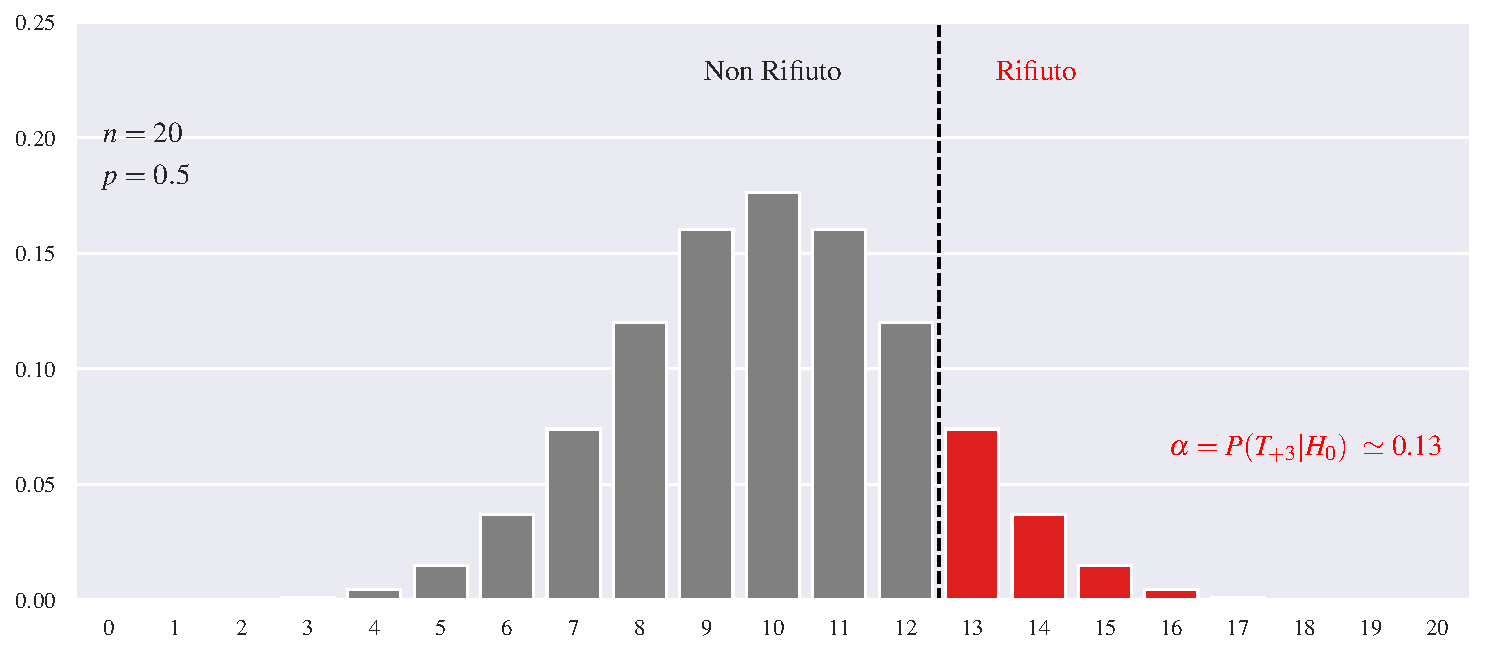
\includegraphics[width=0.9\textwidth]{figure/B-test_01.pdf}


%%%%%%%%%%%%
%%%%%%%%%%%%
%%%%%%%%%%%%
%%%%%%%%%%%%
\clearpage\hfill\textbf{Test Binomiale}\subsection{Test a una coda, errore II tipo}

La probabilità dei falsi negativi può essere espressa in funzione di $p$ (abbiamo solo assunto che $p>1/2$)


\ceq{\hfill \Pr(\neg T_{+k}\mathrel|H_A)}{=}{\Pr(X< k\mathrel|H_A)\quad=\quad\sum^{k-1}_{i=1} {n\choose i}p^i(1-p)^{n-i}}

Consideriamo come prima $k=3$.
Abbiamo {\color{blue}\boldmath\ $\neg T_{+k}=\{0,\dots,12\}$} è la zona di \emph{NON rifiuto.}
Rappresentiamo la distribuzione di $X$ nel caso in cui vale $H_{A}$. Per confronto lo accostiamo al grafico del paragrafo precedente. 

\hfil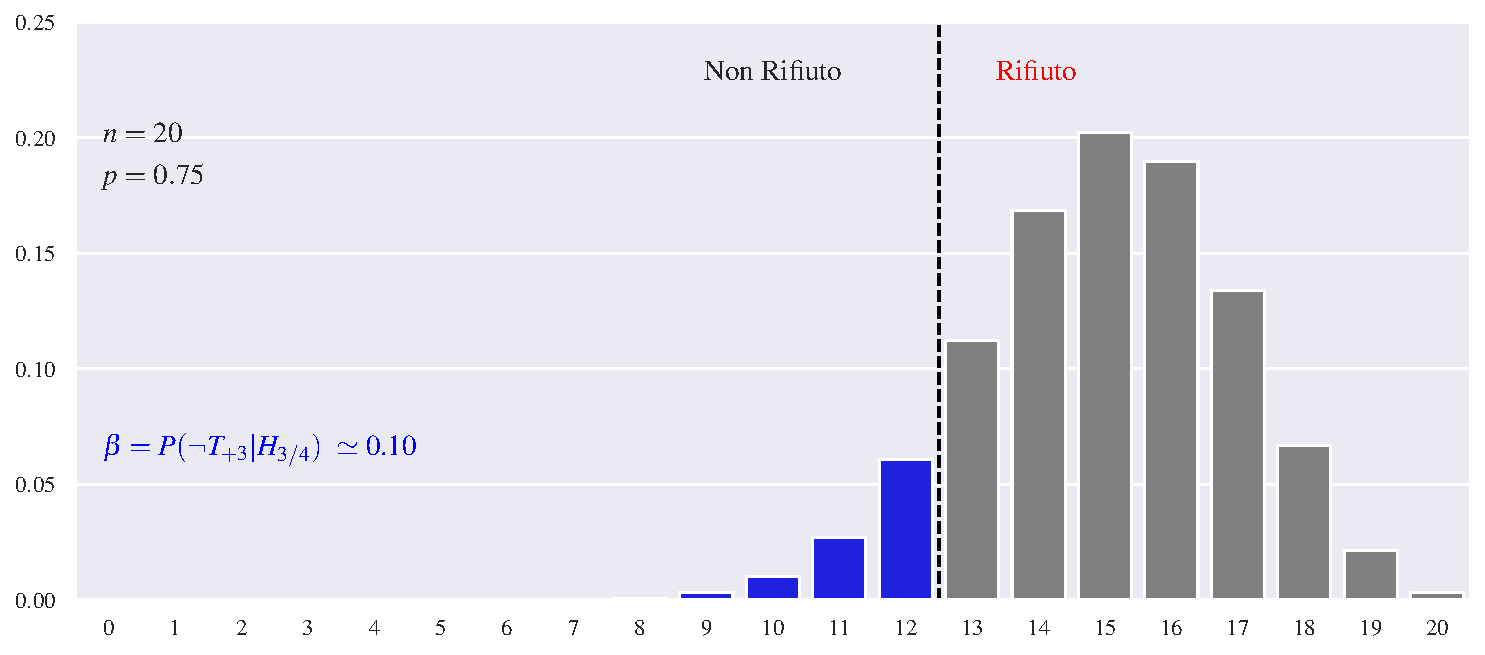
\includegraphics[width=0.9\textwidth]{figure/B-test_02.pdf}

\hfil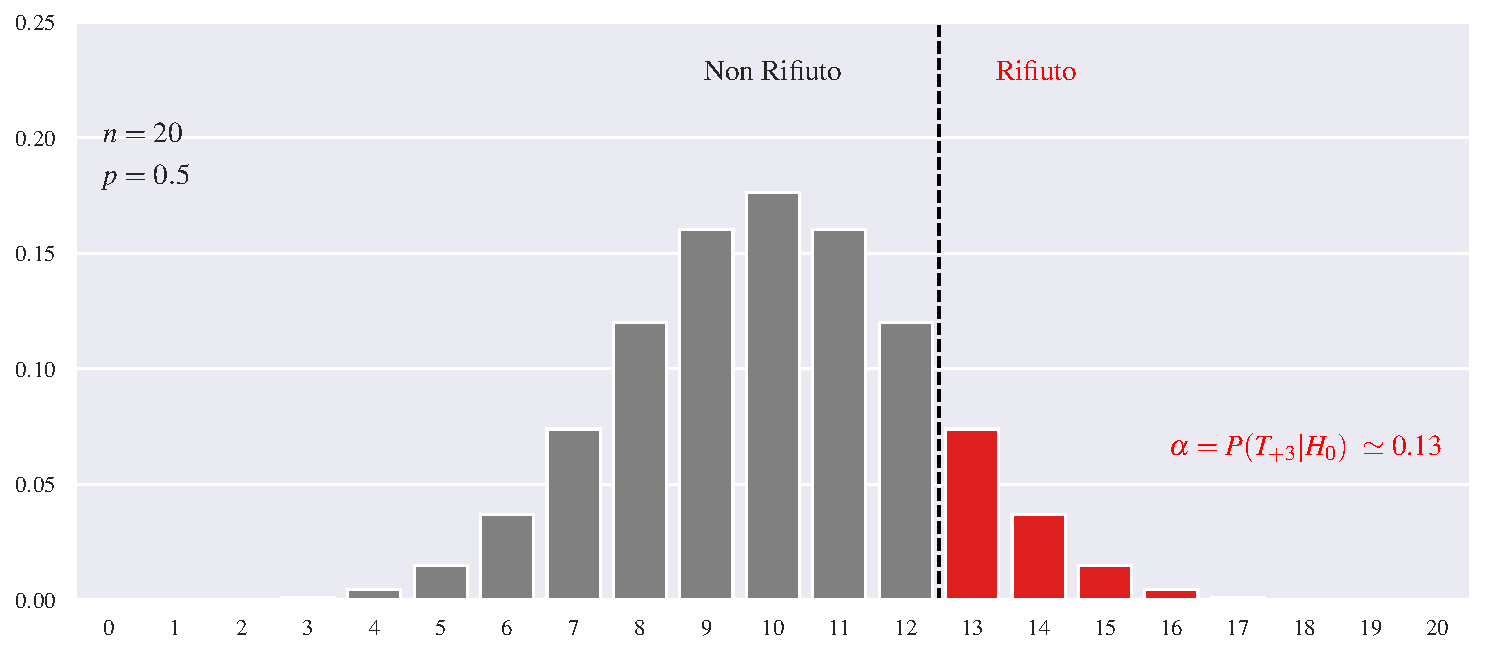
\includegraphics[width=0.9\textwidth]{figure/B-test_01.pdf}




%%%%%%%%%%%%
%%%%%%%%%%%%
%%%%%%%%%%%%
\clearpage\hfill\textbf{Test Binomiale}\subsection{Effect size: \boldmath{$\delta$}}


Cosa possiamo dire se l'ipotesi alternativa fosse stata $H_A:$ $p>1/2$~?

\hfil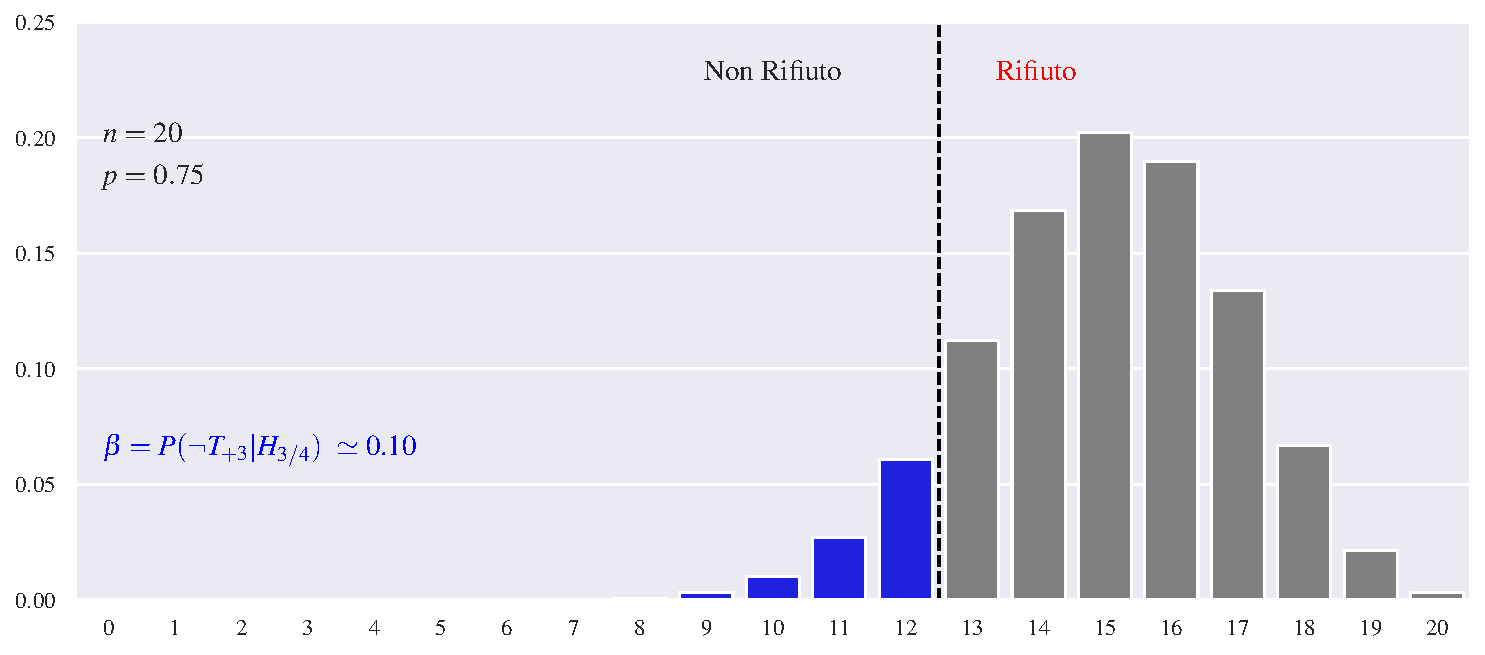
\includegraphics[width=0.9\textwidth]{figure/B-test_02.pdf}

\hfil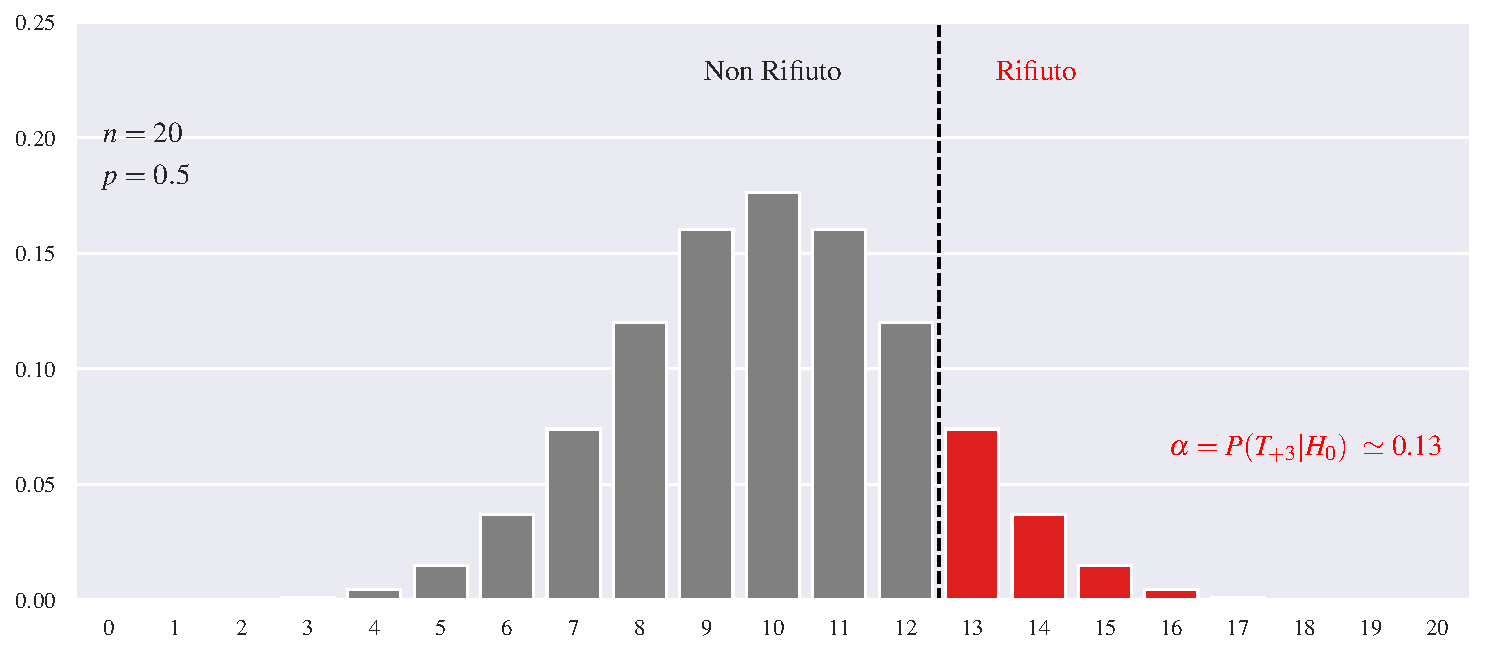
\includegraphics[width=0.9\textwidth]{figure/B-test_01.pdf}

Al crescere di $p$ la distribuzione si sposta verso destra quindi la probabilità di errori del II tipo diminuisce. 
Di converso, se $p$ si sposta verso sinistra e si avvicina a $1/2$  la probabilità d'errore del II tipo aumenta. Al limite quando $p\approx 1/2$ avremo $\alpha+\beta\approx 1$. 
Dobbiamo quindi fissare il minima differenza $\delta$ che riteniamo significativa e prendere come ipotesi alternativa  $H_A:$ $p\ge1/2+\delta$.
Per calcolare $\beta$ abbiamo comunque bisogno di un preciso valore di $p$.
Scegliamo quindi il più sfavorevole $H_A:$ $p=1/2+\delta$.




%%%%%%%%%%%%
%%%%%%%%%%%%
%%%%%%%%%%%%
\clearpage\hfill\textbf{Test Binomiale}\subsection{Test a due code}

Nell'esempio precedente avevamo un'informazione certa sul tipo di difetto delle monete: sapevamo che $p>1/2$. Proviamo a fare senza, avremo quindi

$H_0:$\kern3.5ex $p=1/2$

$H_A:$\kern3ex $p\neq1/2$

Verifichiamo prima che  \textbf{la zona di rifiuto dei paragrafi precedenti NON è adatta\/} alla nuova situazione. 
Il grafici che descrive $\Pr(T_{+3}|H_0)$ rimane invariato (perché l'insieme $H_0$ non è cambiato).
Le cose cambiano drammaticamente se vale $H_A$.

Per semplificare la discussione dell'errore del II tipo fissiamo $\delta=1/4$ e ci mettiamo nei casi più sfavorevoli (sono due ai due lati di $H_0$)

$H_A:$\kern3ex $p=3/4$\quad o\quad $p=1/4$ 

Possiamo immaginare $H_A=H_{{1/4}}\cup H_{{3/4}}$. 
Se sostituiamo $H_A$ con $H_{{3/4}}$ il grafico rimane come quello già discusso. 
Ora però dobbiamo considerare il caso il cui la moneta appartenga all'insieme $H_{{1/4}}$

\hfil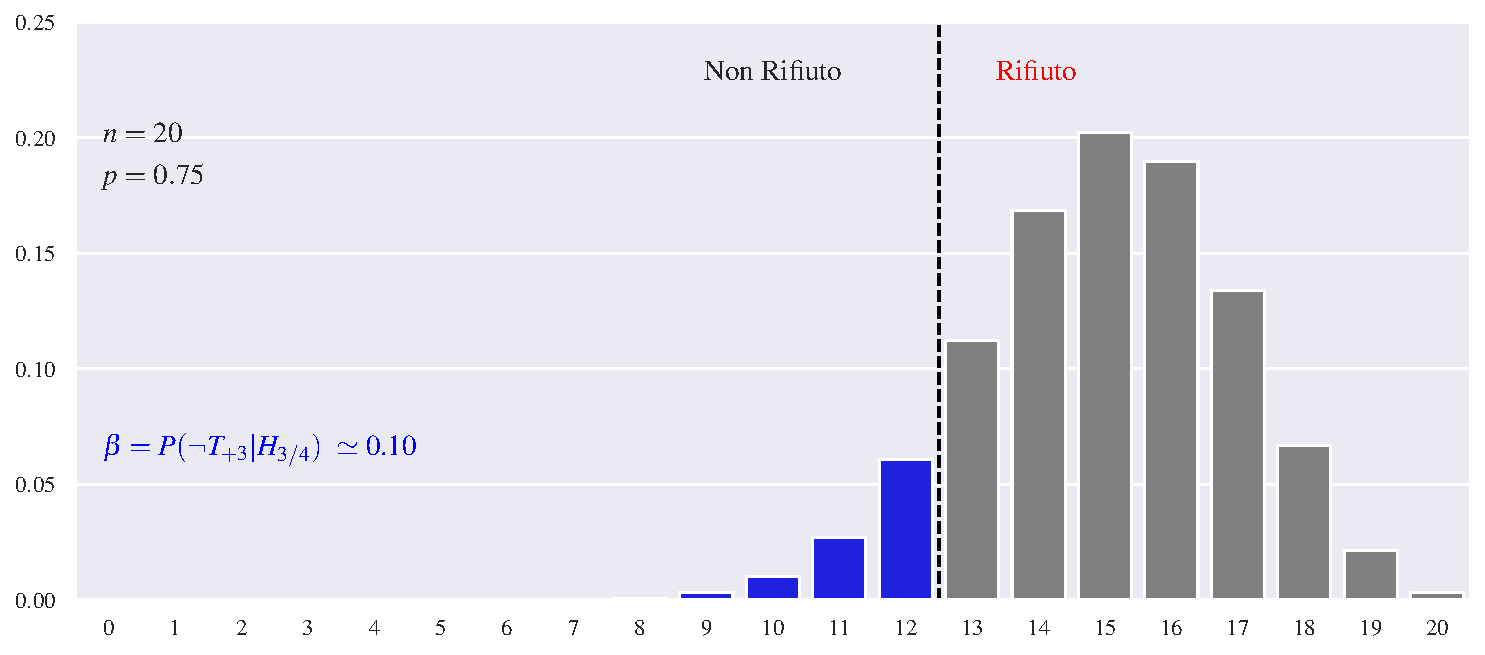
\includegraphics[width=0.9\textwidth]{figure/B-test_02.pdf}

\hfil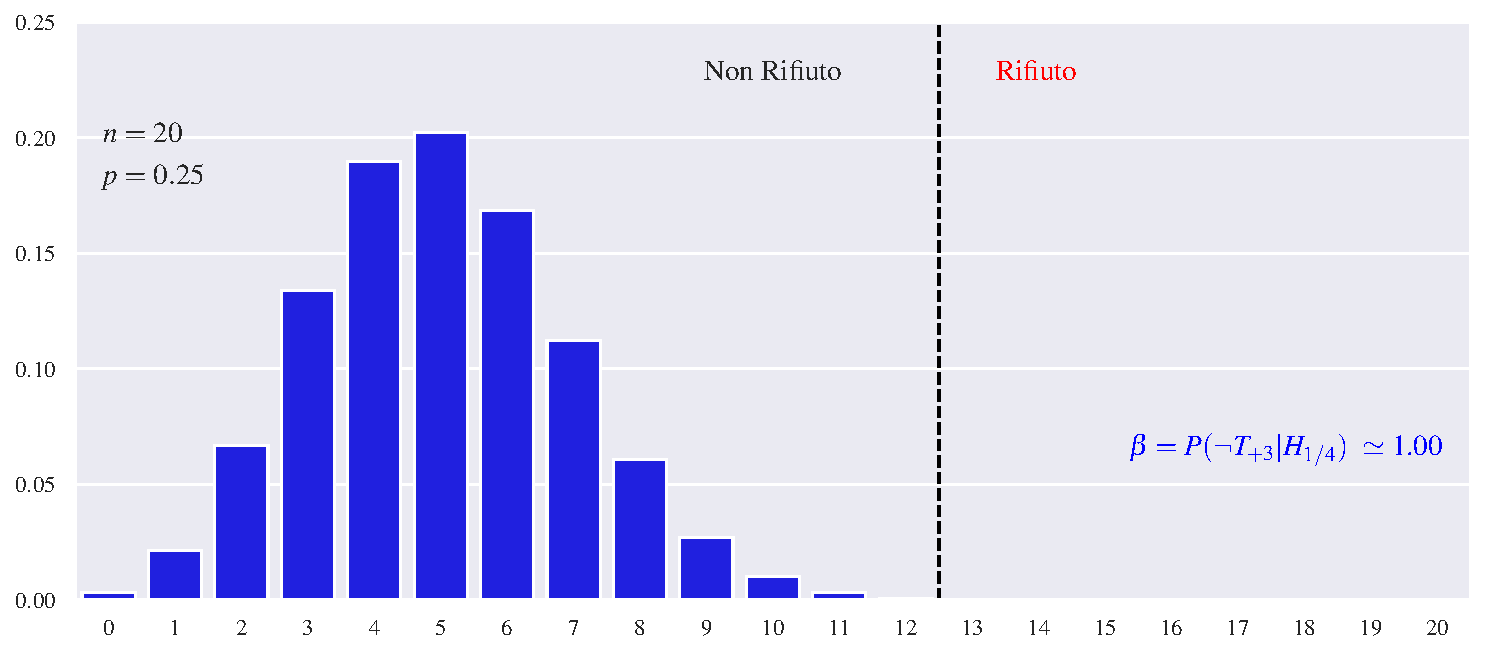
\includegraphics[width=0.9\textwidth]{figure/B-test_03.pdf}


%%%%%%%%%%%%
%%%%%%%%%%%%
%%%%%%%%%%%%
\clearpage\hfill\textbf{Test Binomiale}\subsection{Test a due code, errori I e II tipo}

Per riparare il problema discusso al paragrafo precedente. 
Prendiamo come nuova zona di rifiuto {\color{red}\boldmath $T_{\pm k}\ = \ \{0,\dots,7=n-k\}\cup \{k=13,\dots,20=n\}$}

\hfil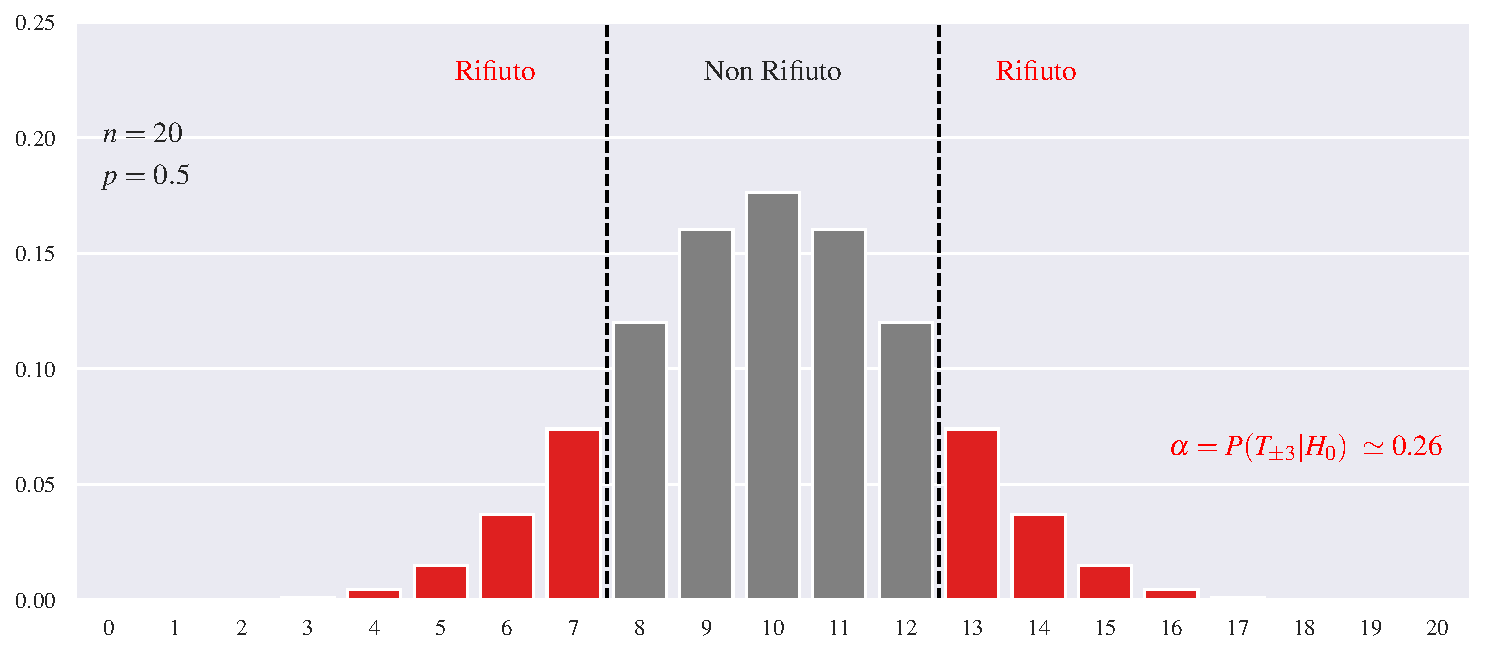
\includegraphics[width=0.9\textwidth]{figure/B-test_04.pdf}

\hfil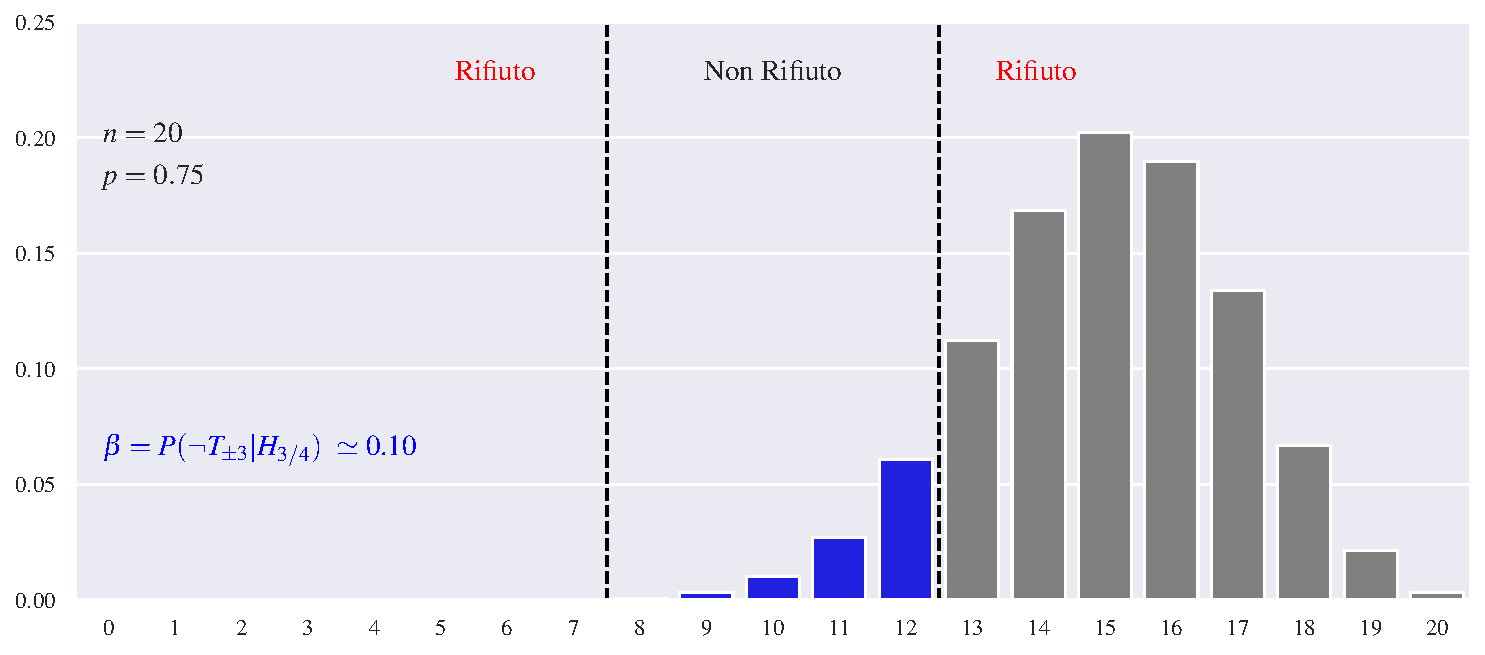
\includegraphics[width=0.9\textwidth]{figure/B-test_05.pdf}

\hfil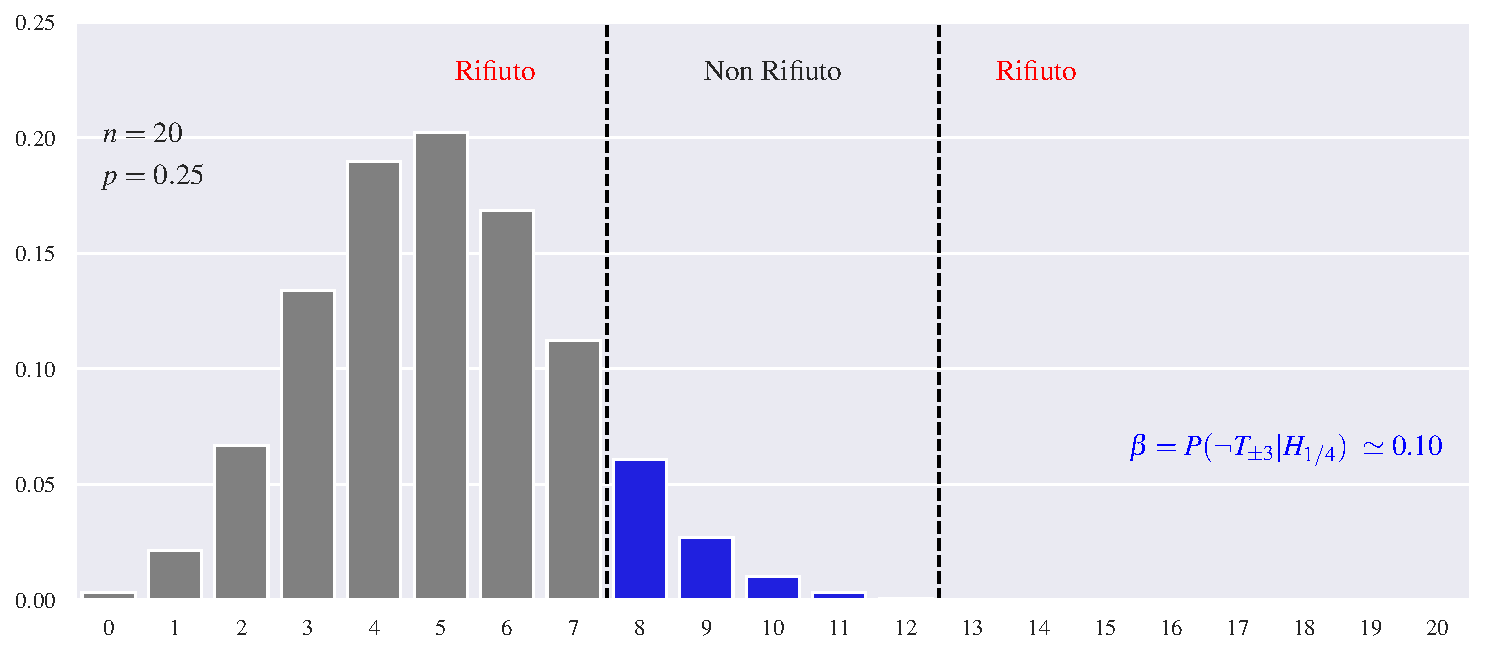
\includegraphics[width=0.9\textwidth]{figure/B-test_06.pdf}




%%%%%%%%%%%%
%%%%%%%%%%%%
%%%%%%%%%%%%
\clearpage\hfill\textbf{Test Binomiale}
\subsection{Test a due code, con campione più ampio}

Supponiamo di raddoppiare la dimensione del campione ($n=40$). Aggiustiamo la zona di rifiuto allo stesso modo ($k=6$): 

\hfil$T_{\pm6}=\{0,\dots,14=n/2-k\}\cup \{k+n/6=26,\dots,40\}$

Entrambi gli errori diminuiscono.


\hfil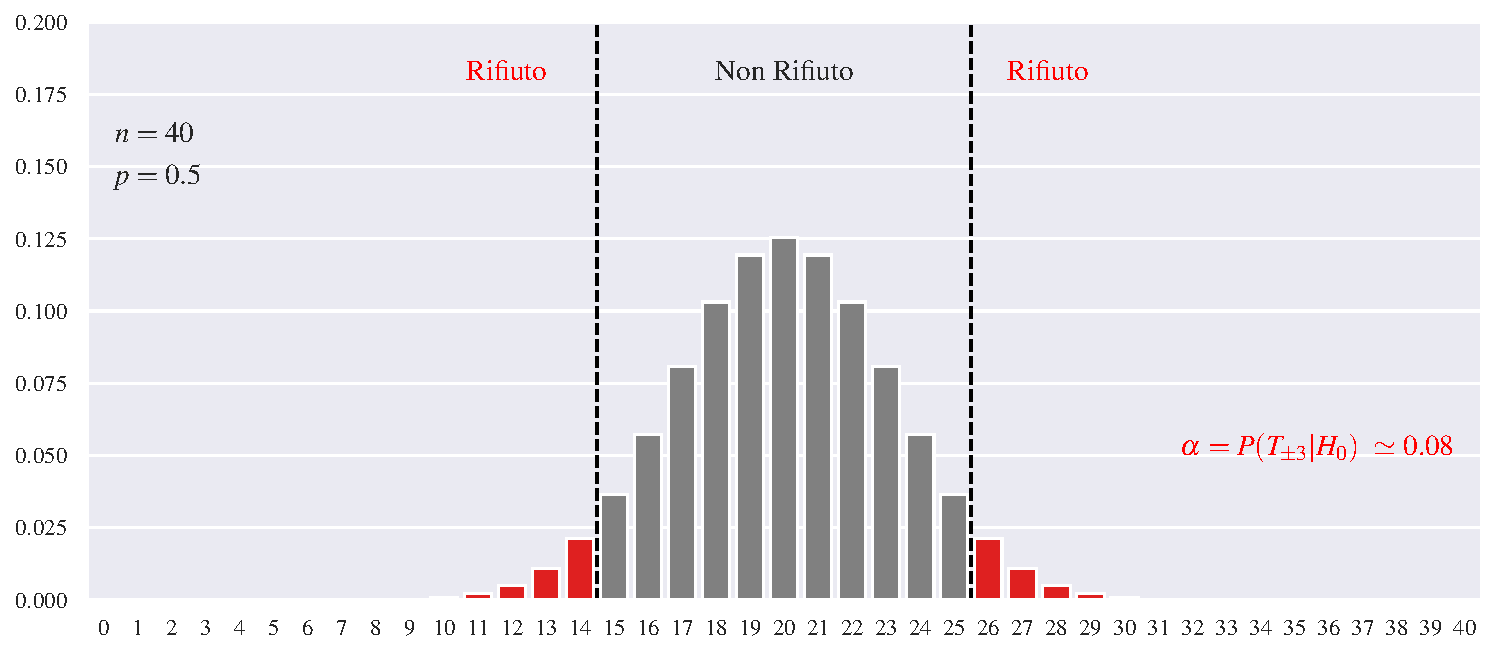
\includegraphics[width=0.9\textwidth]{figure/B-test_07.pdf}

\hfil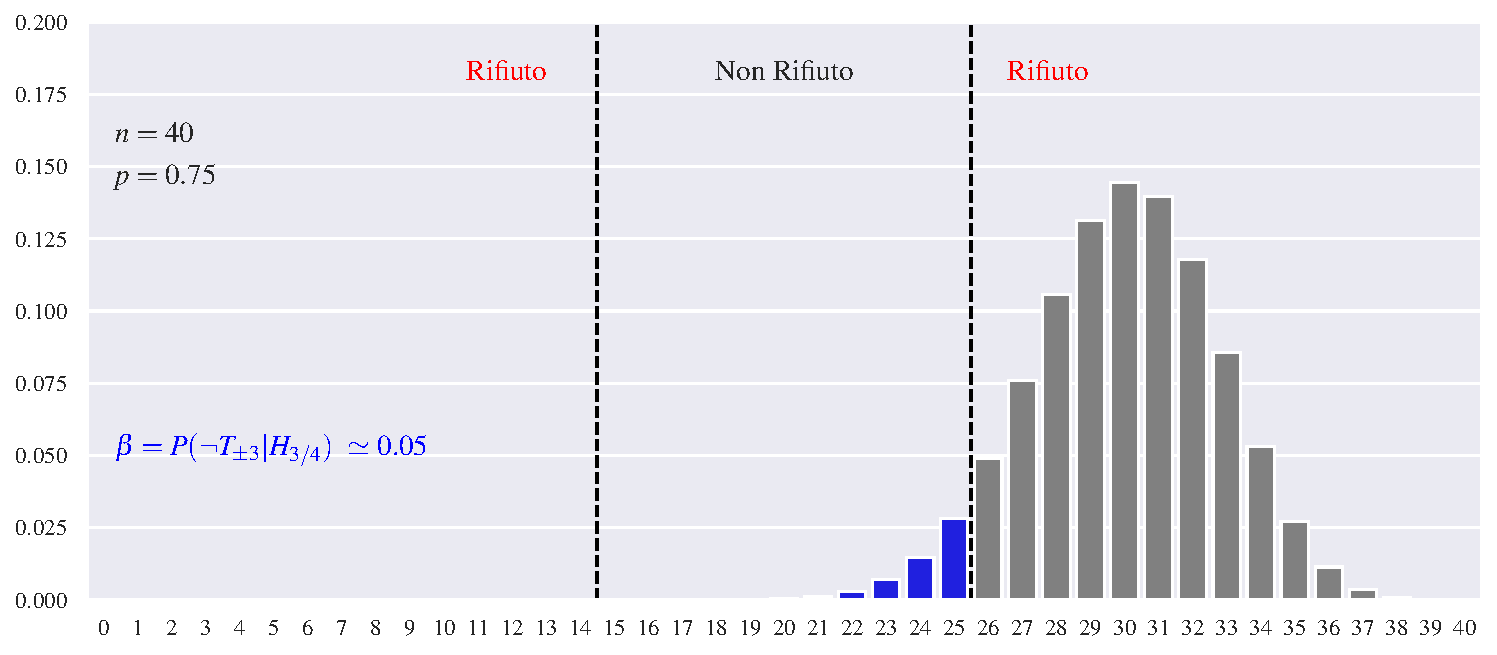
\includegraphics[width=0.9\textwidth]{figure/B-test_08.pdf}

\hfil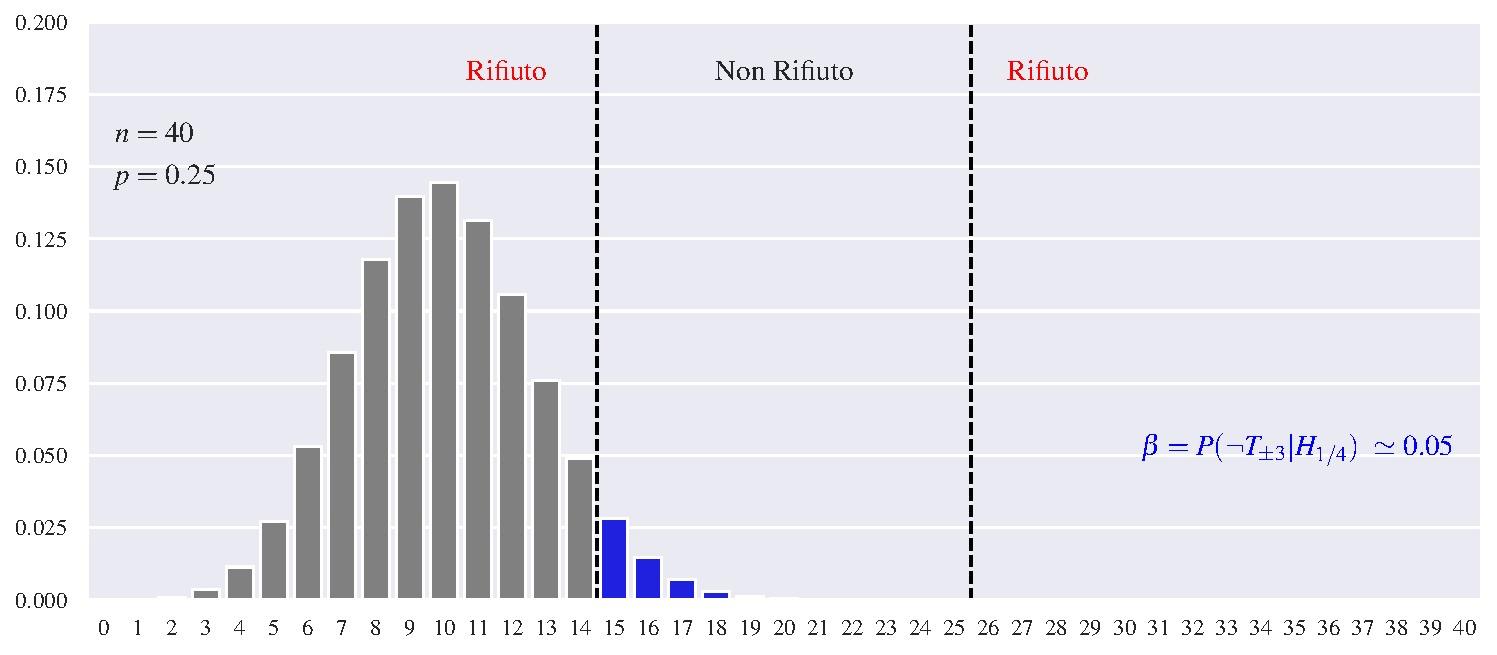
\includegraphics[width=0.9\textwidth]{figure/B-test_09.pdf}



\begin{comment}
%%%%%%%%%%%%
%%%%%%%%%%%%
%%%%%%%%%%%%
\clearpage\hfill\textbf{Test Binomiale}
\subsection{Standardizzazione (1)}

Il confronto tra i test con $n=20, 40$ non é immediato (vedi la trasformazione della zona di rifiuto). Per facilitare il confronto tipicamente la variabile viene standardizzata. 

Se $X\sim B(n,p)$ allora, ricordando che la media è $\mu=np$ e la varianza è $\sigma^2=np(1-p)$, la variabile standardizzata diventa

\ceq{\hfill Z}{=}{\frac{X-\mu}{\sigma}}

\ceq{\hfill }{=}{\frac{X-np}{\rule{0ex}{3ex}\sqrt{np\big(1-p\big)}}}


Gli esempi considerati (con $n=20,40$ e $k=13,26$) diventano: 

\hfil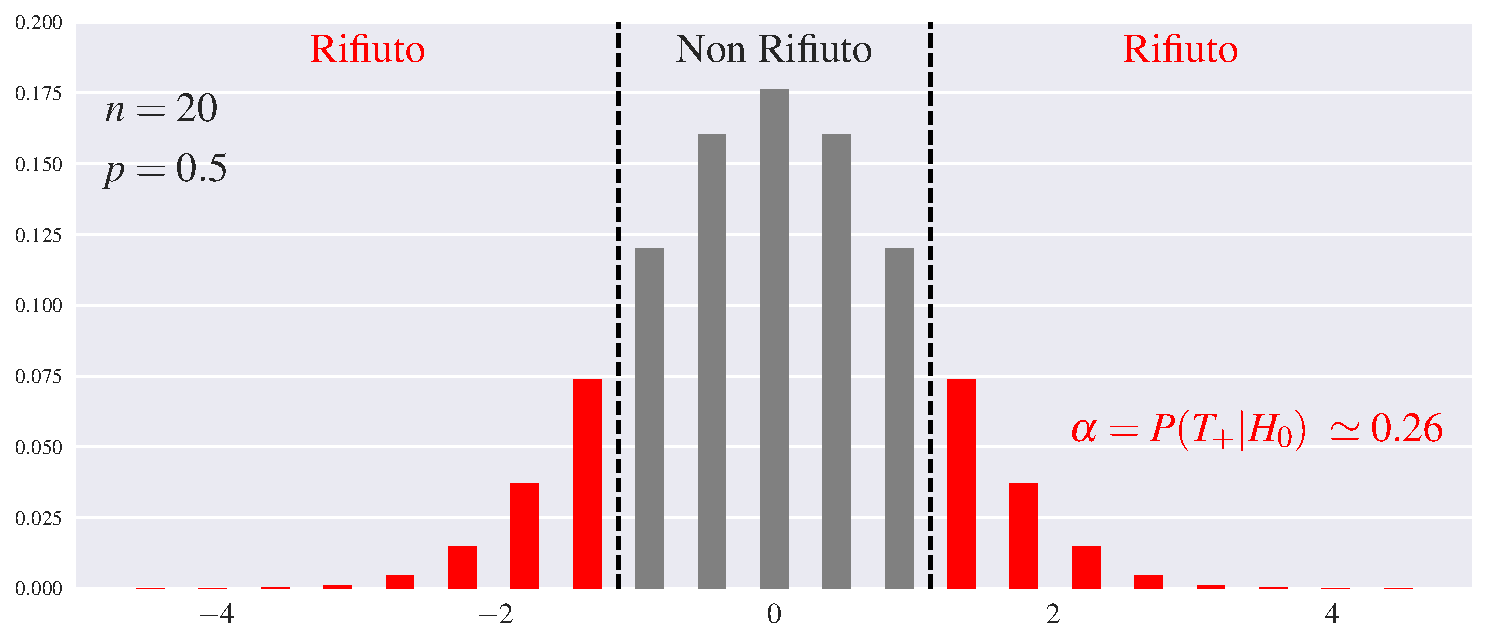
\includegraphics[width=0.9\textwidth]{figure/B-test-standard_01.pdf}

\hfil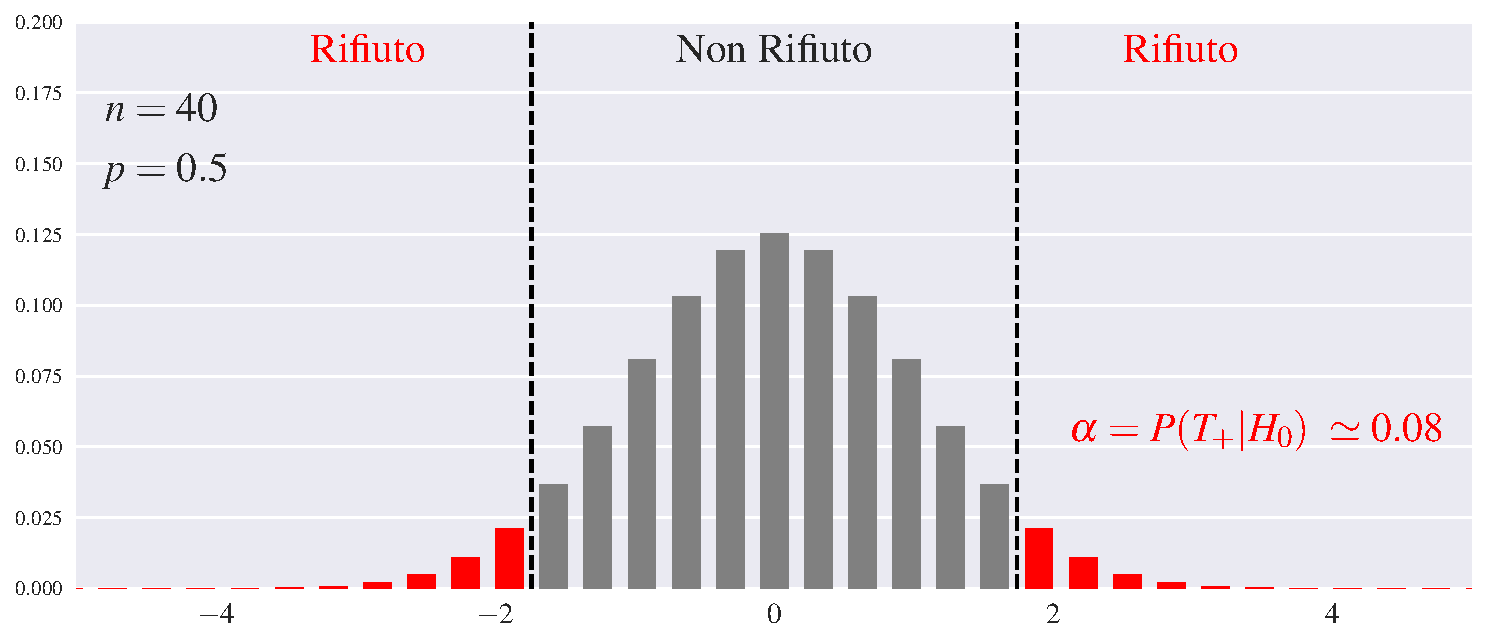
\includegraphics[width=0.9\textwidth]{figure/B-test-standard_02.pdf}


%%%%%%%%%%%%
%%%%%%%%%%%%
%%%%%%%%%%%%
\clearpage\hfill\textbf{Test Binomiale}
\subsection{Standardizzazione (2)}

Si noti che le regioni di rifiuto non sono le stesse. In effetti


\ceq{\hfill\frac{k-np}{\rule{0ex}{3ex}\sqrt{np\big(1-p\big)}}}{=}{1.34}\qquad se $n=20$, \ $k=13$, \ $p=05$


\ceq{}{=}{1.90}\qquad se $n=40$, \ $k=26$, \ $p=05$


Se per entrambi i casi prendiamo la stessa regione di rifiuto misurata in punteggio $Z$, diciamo $(-\infty, -1.34]\ \cup\ [1.34, +\infty)$, che corrisponde a $k=24$ o $25$,  avremmo ottenuto praticamente lo stesso $\alpha$. Infatti una volta standardizzate le due distribuzioni diventano estremamente simili. Lo scopo dela standardizzazione è rendere evidenti queste similitudini.  


\hfil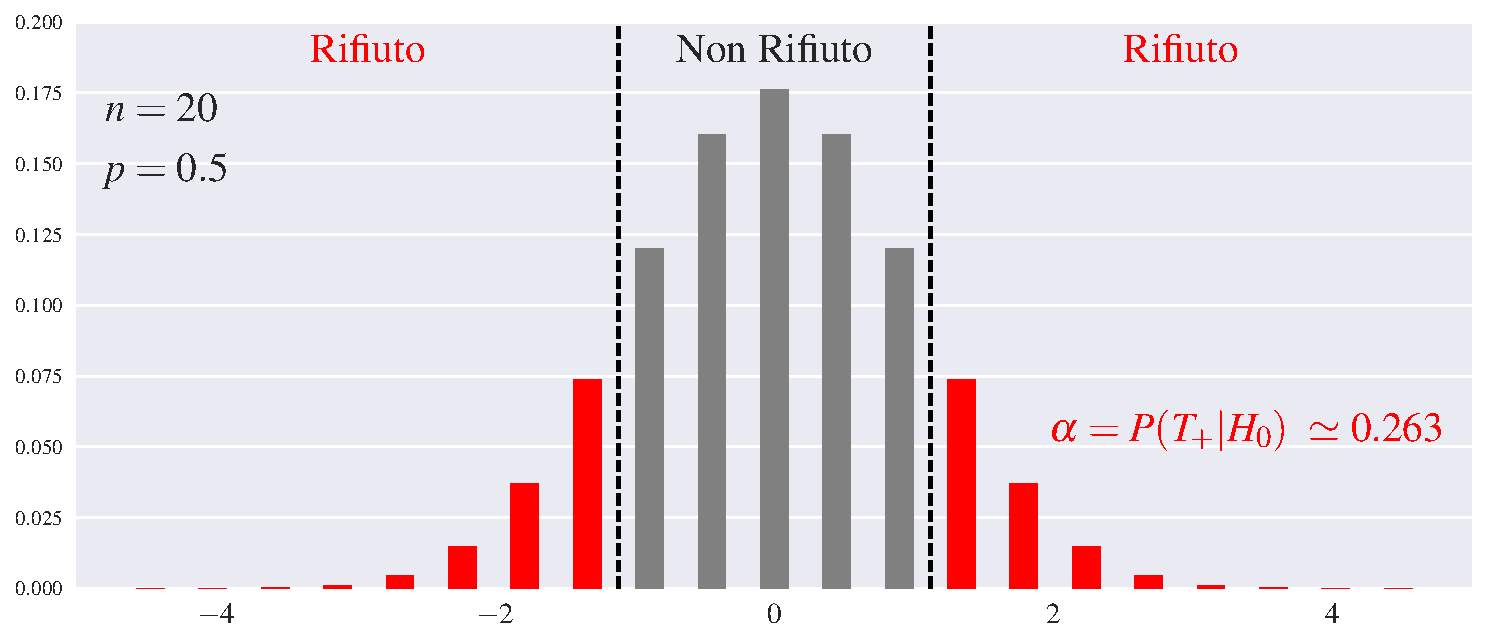
\includegraphics[width=0.9\textwidth]{figure/B-test-standard2_01.pdf}

\hfil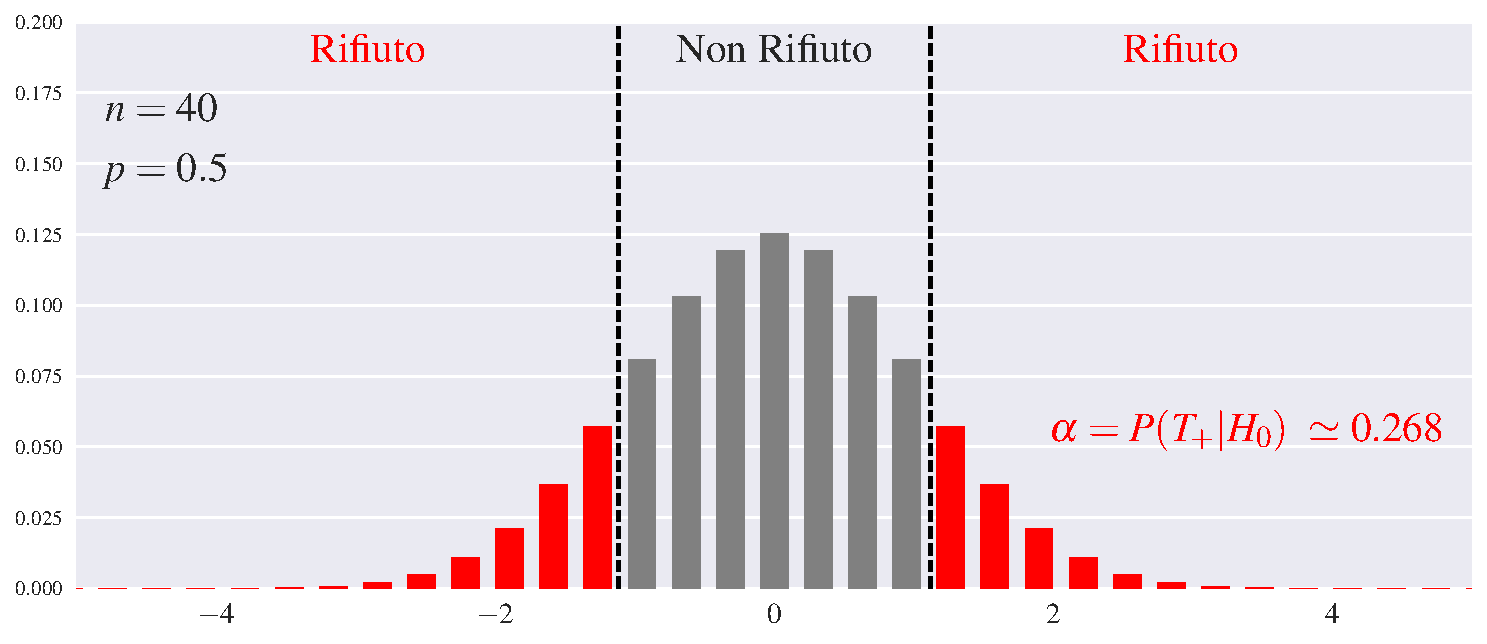
\includegraphics[width=0.9\textwidth]{figure/B-test-standard2_02.pdf}


  
\end{comment}

%%%%%%%%%%%%
%%%%%%%%%%%%
%%%%%%%%%%%%
\clearpage\
\hfill\textbf{{\color{brown}\hyperref[test_ipotesi]{Test di ipotesi \faShare}}}
\subsection{Scatola di biglie colorate (esercizio in formato esame)}
\label{Scatola di biglie colorate}

Un impianto di produzione di una fabblica riempie scatole con due tipi di biglie: rosse e blu.
È stato garantito al cliente che le scatole contengono almeno il $40\%$ di biglie rosse con una tolleranza del $5\%$.

Per controllare la qualità delle scatole confezionate preleviamo un campione $100$ biglie. Sia $N$ la v.a. che ritorna il numero di biglie rosse nel campione.


\textbf{Domande.}

\begin{itemize}
\item[1.] Qual è l'potesi nulla?

\item[2.] Qual è l'potesi alternativa?

\item[3.] Qual è l'effect size?

\item[4.] Che confezioni devono essere scartate se vogliamo che il  $95\%$ delle confezioni non conformi al nostro obbiettivo vengano scartate?

\item[5.] Dato il risultato al punto precedente qual è la probabilità $\alpha$ di un erore del I tipo? 
\end{itemize}

Si risponda assumendo note le funzioni in calce.


\textbf{Risposte.} Definiamo $n=100$,\quad $\beta=0.05$,\quad $p_0=0.4$.

\begin{itemize}
\item[1.] $H_0$: \ $p=p_0$ dove $p$ è la frazione di biglie rosse nella confezione in esame

\item[2.] $H_A$: $p< p_0$ 

\item[3.] $\delta=0.05$

\item[4.] Scartiamo la confezione se $N\le x$. 
Dove $x$ è calcolato sapendo che\smallskip

$1-\beta=\Pr\big(N\le x \mathbin\big| p=p_0-\delta\big)=\Pr(X\le x)$ dove $X\sim{\rm B}(n,p_0-\delta)$\smallskip

\hfill
$x =$ {\tt qbinom}$(1-\beta,n,p_0-\delta).$

\item[5.] $\alpha=\Pr\big(N\le x \mathbin\big| p=p_0\big)=\Pr(X\le x)$  dove $X\sim{\rm B}(n,p_0)$\smallskip

\hfill
$\alpha =$ {\tt pbinom}$(x,n,p_0)$.
\end{itemize}

\vfill
\parskip1ex
{\hrulefill\scriptsize

{\tt pbinom(x,n,p)}=$P(X\le x)$, per $X\sim B(n,p)$
\hfill 
{\tt qbinom($\alpha$,n,p)=x},  dove $P(X\le x)=\alpha$ per $X\sim B(n,p)$

{\tt pnorm(z)}=$P(Z\le z)$, per $Z\sim N(0,1)$
\hfill 
{\tt qnorm($\alpha$)=z},  dove $P(Z\le z)=\alpha$ per $Z\sim N(0,1)$

{\tt pt(t,$\nu$)} = $P(T\le t)$ per $T\sim t(\nu)$
\hfill
{\tt qt($\alpha$,$\nu$)=t}, dove $P(T\le t)=\alpha$ per $T\sim t(\nu)$

{\tt pchisq(q,k)} = $P(Q\le q)$, per $Q\sim \chi^2_k$
\hfill
{\tt qchisq($\alpha$,k)=q},  dove $P(Q\le q)=\alpha$ per $Q\sim \chi^2_k$
\par
}

%%%%%%%%%%%%
%%%%%%%%%%%%
%%%%%%%%%%%%
\clearpage\
\hfill\textbf{{\color{brown}\hyperref[test_ipotesi]{Test di ipotesi \faShare}}}
\subsection{Prevalenza mancinismo 1 (esercizio in formato esame)}
\label{Prevalenza mancinismo 1}

Il $10\%$ è delle persone sono mancine. Ci chiediamo se la caratteristica sia ereditaria. Eseguiamo il seguente esperimento. Selezioniamo un campione di $1000$ persone con almeno un genitore mancino e misuriamo la frequenza di mancini. Concludiamo che la caratteristica \`e ereditaria se pi\`u di $115$ individui sono mancini.

\textbf{Domande.}

\begin{itemize}
\item[1.] Qual è l'potesi nulla?

\item[2.] Qual è l'potesi alternativa?

\item[3.] Che test stiamo facendo?

\item[4.] Qual è la significatività del test?

\item[5.] Supponiamo che un leggero fattore ereditario renda la prevalenza del mancinismo tra i figli di un genitore mancino $\ge12\%$. Stimare la probabilità che questa dipendenza ereditaria non venga rilevata dal test. 

\item[6.] Qual è la potenza del test nel caso descritto sopra.
\end{itemize}

Si risponda assumendo note le funzioni in calce.

\textbf{Risposte.} \ Definiamo: \ $n=1000$,\hfil
$x=115$,\hfil
$p_0=0.10$,\hfil
$p_1=0.12$,\hfil
$\alpha=0.01$\hfil

\begin{itemize}
\item[1.] $H_0$: \ $p=p_0$ dove $p$ è la prevalenza del mancinismo tra i figli di mancini.
\item[2.] $H_A$: \ $p>p_0$ 
\item[3.] Test binomiale a una coda.
\item[4.] $\Pr(X> x)$ dove $X\sim B(n,p_0)$ ovvero {\tt 1-pbinom($x$,$n$,$p_0$)}
\item[5.] $\beta=\Pr(X\le x)$ dove $X\sim B(n,p_1)$ ovvero {\tt pbinom($x$,$n$,$p_1$)}
\item[6.]  La potenza è $1-\beta$.
\end{itemize}


\vfill
\parskip1ex
{\hrulefill\scriptsize

{\tt pbinom(x,n,p)}=$P(X\le x)$, per $X\sim B(n,p)$
\hfill 
{\tt qbinom($\alpha$,n,p)=x},  dove $P(X\le x)=\alpha$ per $X\sim B(n,p)$

{\tt pnorm(z)}=$P(Z\le z)$, per $Z\sim N(0,1)$
\hfill 
{\tt qnorm($\alpha$)=z},  dove $P(Z\le z)=\alpha$ per $Z\sim N(0,1)$

{\tt pt(t,$\nu$)} = $P(T\le t)$ per $T\sim t(\nu)$
\hfill
{\tt qt($\alpha$,$\nu$)=t}, dove $P(T\le t)=\alpha$ per $T\sim t(\nu)$

{\tt pchisq(q,k)} = $P(Q\le q)$, per $Q\sim \chi^2_k$
\hfill
{\tt qchisq($\alpha$,k)=q},  dove $P(Q\le q)=\alpha$ per $Q\sim \chi^2_k$
\par
}

%%%%%%%%%%%%
%%%%%%%%%%%%
%%%%%%%%%%%%
\clearpage\
\hfill\textbf{{\color{brown}\hyperref[test_ipotesi]{Test di ipotesi \faShare}} (richiede \hyperref[pvalore]{p-valore \faShare})} 
\subsection{Prevalenza mancinismo 2 (esercizio in formato esame)}
\label{Prevalenza mancinismo 2}

Il $10\%$ è delle persone sono mancine. Ci chiediamo se la caratteristica sia ereditaria. Eseguiamo il seguente esperimento. Selezioniamo un campione di $1000$ persone con almeno un genitore mancino e misuriamo la frequenza di mancini. Otteniamo $112$ mancini. 

\textbf{Domande}

\begin{itemize}
\item[1.] Qual è l'potesi nulla?

\item[2.] Qual è l'potesi alternativa?

\item[3.] Che test possiamo fare?

\item[4.] Qual è il p-valore ottenuto dai dati?
\end{itemize}
Si risponda assumendo note le funzioni in calce.

\textbf{Risposte} \ Definiamo: \ $n=1000$,\quad
$x=112$,\quad
$p_0=0.10$.

\begin{itemize}
\item[1.] $p=p_0$ dove $p$ è la prevalenza di mancini tra i figli di genitori mancini
\item[2.]  $p>p_0$ 
\item[3.] Test binomiale a una coda
\item[4.] 


p-valore$\ =\ \Pr\big(X\ge x\ \mathbin\big|\ p=p_0\big)$, dove $X\sim{\rm B}(n,p_0)$ \medskip

\phantom{p-valore}$\ =\ 1 -{\tt  pbinom}(x,n,p_0)$
\end{itemize}


\vfill
\parskip1ex
{\hrulefill\scriptsize

{\tt pbinom(x,n,p)}=$P(X\le x)$, per $X\sim B(n,p)$
\hfill 
{\tt qbinom($\alpha$,n,p)=x},  dove $P(X\le x)=\alpha$ per $X\sim B(n,p)$

{\tt pnorm(z)}=$P(Z\le z)$, per $Z\sim N(0,1)$
\hfill 
{\tt qnorm($\alpha$)=z},  dove $P(Z\le z)=\alpha$ per $Z\sim N(0,1)$

{\tt pt(t,$\nu$)} = $P(T\le t)$ per $T\sim t(\nu)$
\hfill
{\tt qt($\alpha$,$\nu$)=t}, dove $P(T\le t)=\alpha$ per $T\sim t(\nu)$

{\tt pchisq(q,k)} = $P(Q\le q)$, per $Q\sim \chi^2_k$
\hfill
{\tt qchisq($\alpha$,k)=q},  dove $P(Q\le q)=\alpha$ per $Q\sim \chi^2_k$
\par
}


%%%%%%%%%%%%
%%%%%%%%%%%%
%%%%%%%%%%%%
\clearpage\
\hfill\textbf{{\color{brown}\hyperref[distribuzione normale]{La distribuzione normale \faShare}}}
\section{Z-test}
\label{Z-test}
\subsection{Test a una coda}
Si sospetta che una certa terapia faccia aumentare la pressione diastolica. Nella popolazione generale la pressione diastolica ha distribuzione $N(\mu_0,\sigma^2)$ con $\mu_0=75$ e $\sigma=9.5$. 

Assumiamo che tra i pazienti in terapia la pressione diastolica sia distribuita normalmente con media ignota $\mu$ e con la stessa deviazione standard della popolazione generale. Vogliamo testare le seguenti ipotesi:

$H_0:$\kern3.5ex $\mu=\mu_0$

$H_A:$\kern3ex $\mu>\mu_0$

Il test consiste nel misurare la pressione ad un campione di $n$ pazienti e di questi dati calcolare la media. Abbiamo quindi la seguente statistica

\ceq{\hfill \bar X}{=}{\frac1n\sum_{i=1}^nX_i}

Dove $X_i$ è la v.a.\@ che dà la pressione dell'$i$-esimo paziente del campione. Rigetteremo $H_0$ se il
valore ottenuto è suporiore ad un certo $x_\alpha$ che vogliamo fissare in modo che l'errore I tipo risulti uguale ad $\alpha$. Quindi $x_\alpha$ dev'essere tale che $x_\alpha$ tale che $\Pr(\bar X>x_\alpha)=\alpha$.

Se $H_0$ è vera, $\bar X\sim N\bigg(\mu_0,\dfrac{\sigma^2}{n}\bigg)$.

Se $H_A$ è vera, $\bar X\sim N\bigg(\mu,\dfrac{\sigma^2}{n}\bigg)$ per qualche $\mu>\mu_0$.

% Non è necessario, ma conviene sempre ridursi alla normale standard: $\dfrac{\bar X-\mu_0}{\sigma/\sqrt{n}}$ ha distribuzione normale standard $Z$.
% 
% Vogliamo $x_\alpha$ tale che $\Pr(Z>\dfrac{x_\alpha-\mu_0}{\sigma/\sqrt{n}})=\alpha$



%%%%%%%%%%%%
%%%%%%%%%%%%
%%%%%%%%%%%%
\clearpage\subsection{Una coda, errore I e II tipo}


Qui rappresentiamo gli errori del I e II tipo per campioni di dimensione $n=20$ e $n= 40$ e con un $x_\alpha$ scelto in moto tale da avere $\alpha=5\%$. Per gli errori del II tipo prendiamo $\delta=5$.

\hfil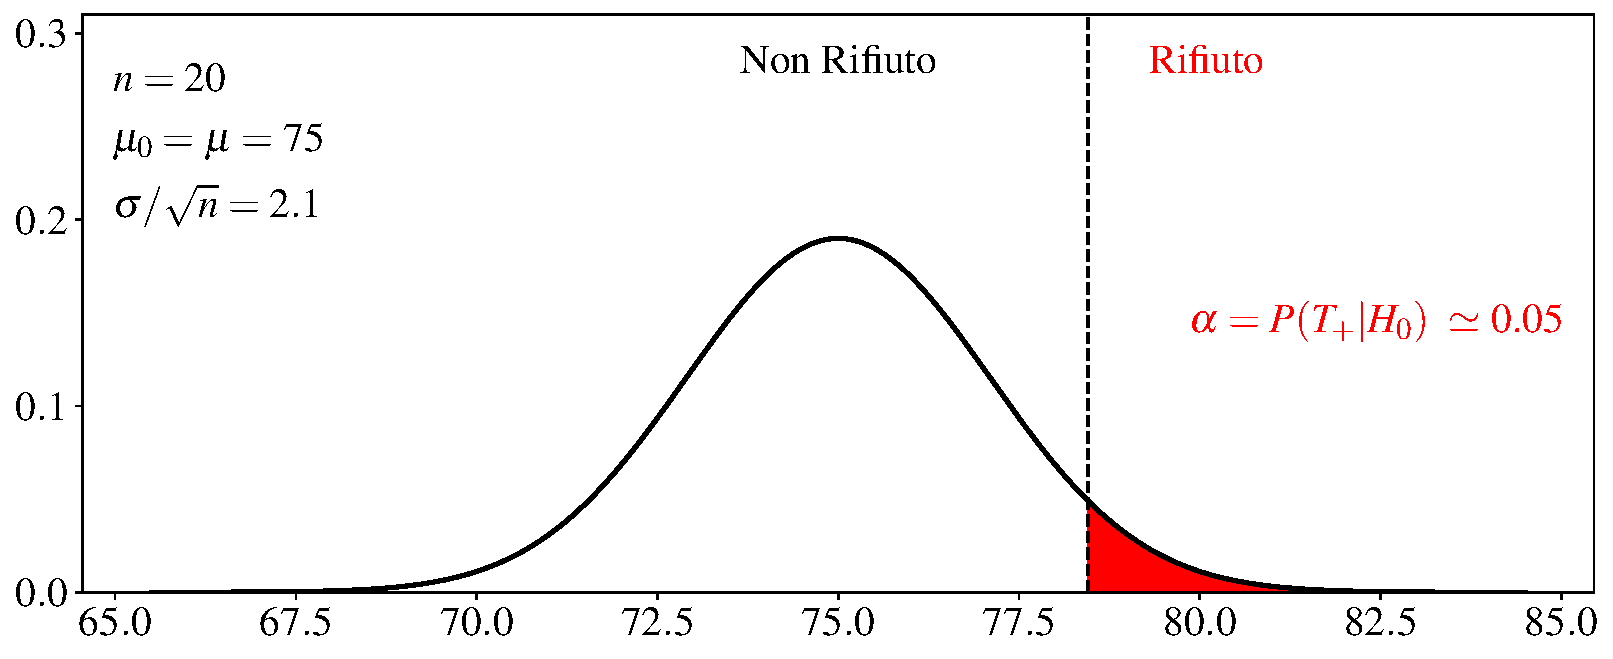
\includegraphics[width=0.8\textwidth]{figure/Z-test_01.pdf}

\hfil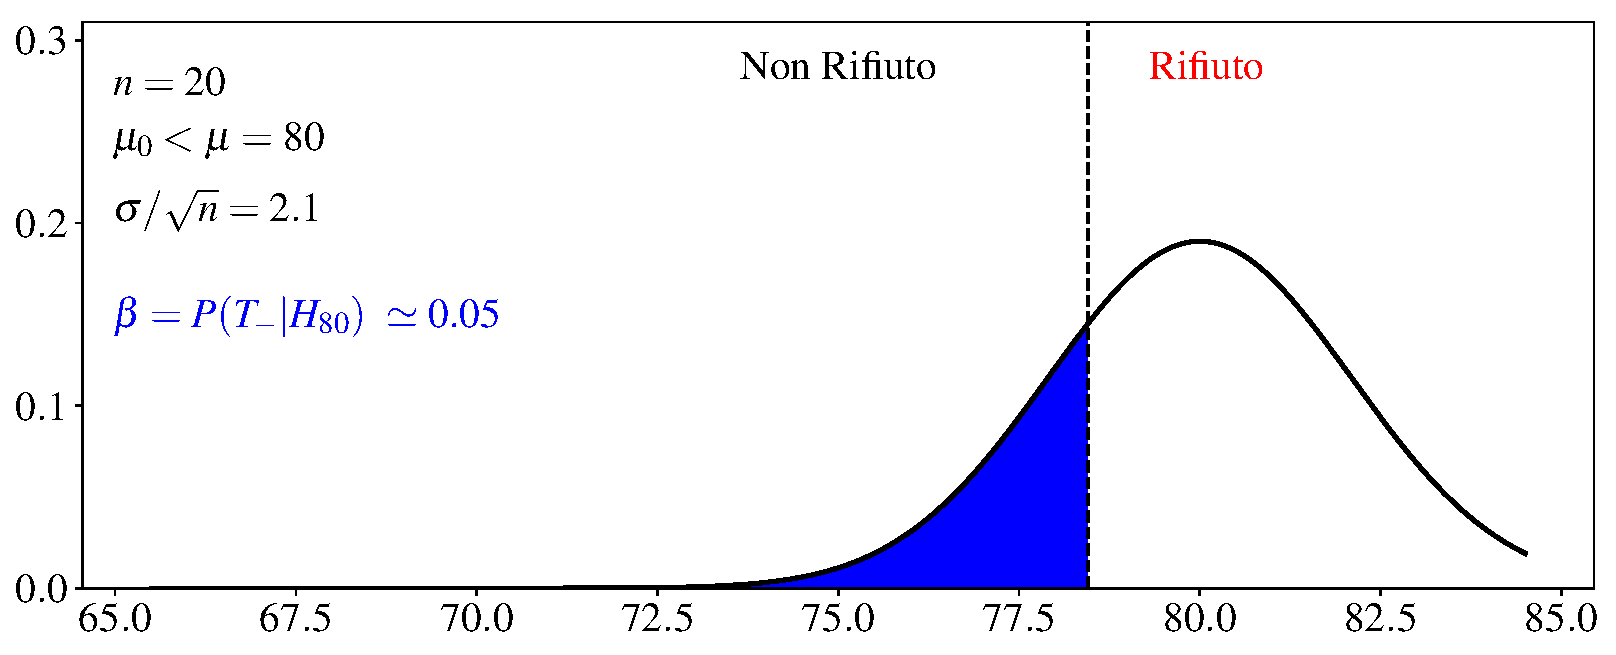
\includegraphics[width=0.8\textwidth]{figure/Z-test_02.pdf}

\hfil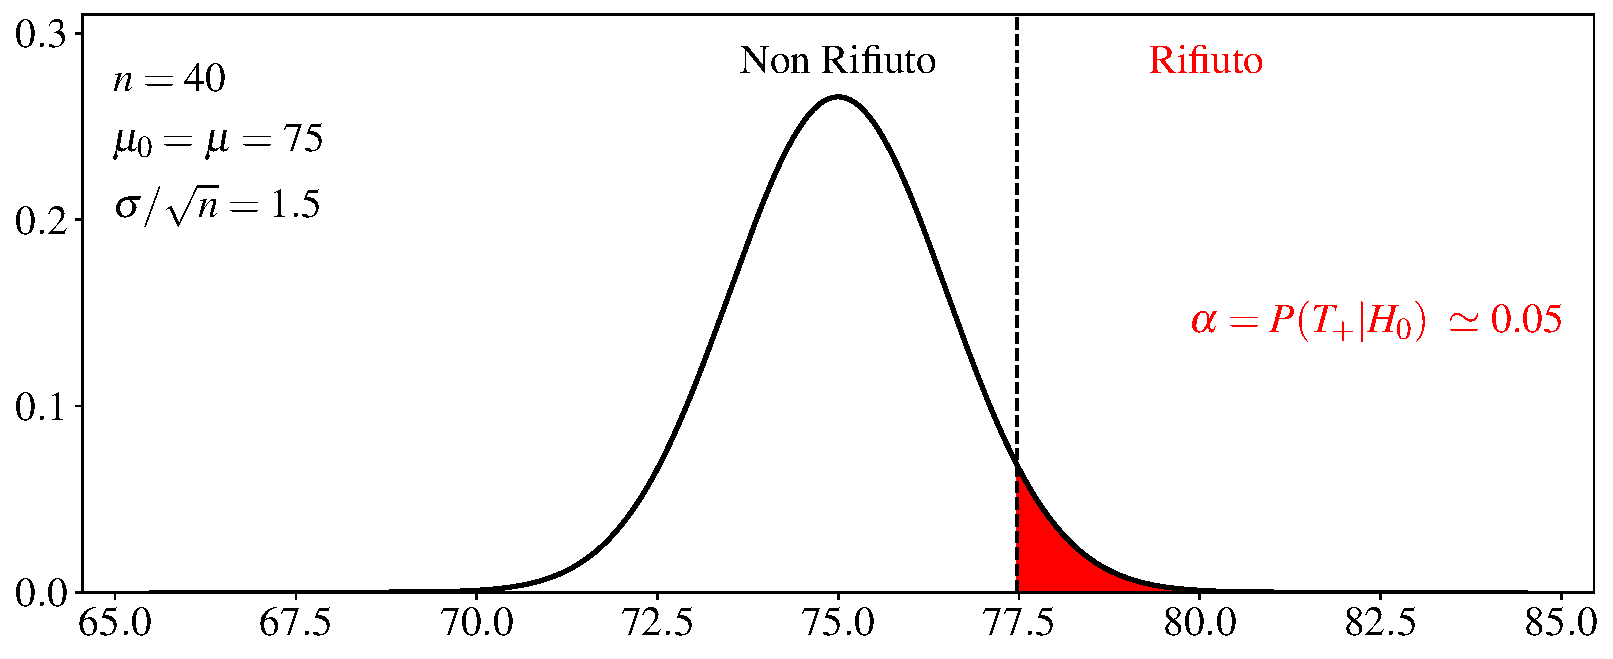
\includegraphics[width=0.8\textwidth]{figure/Z-test_03.pdf}

\hfil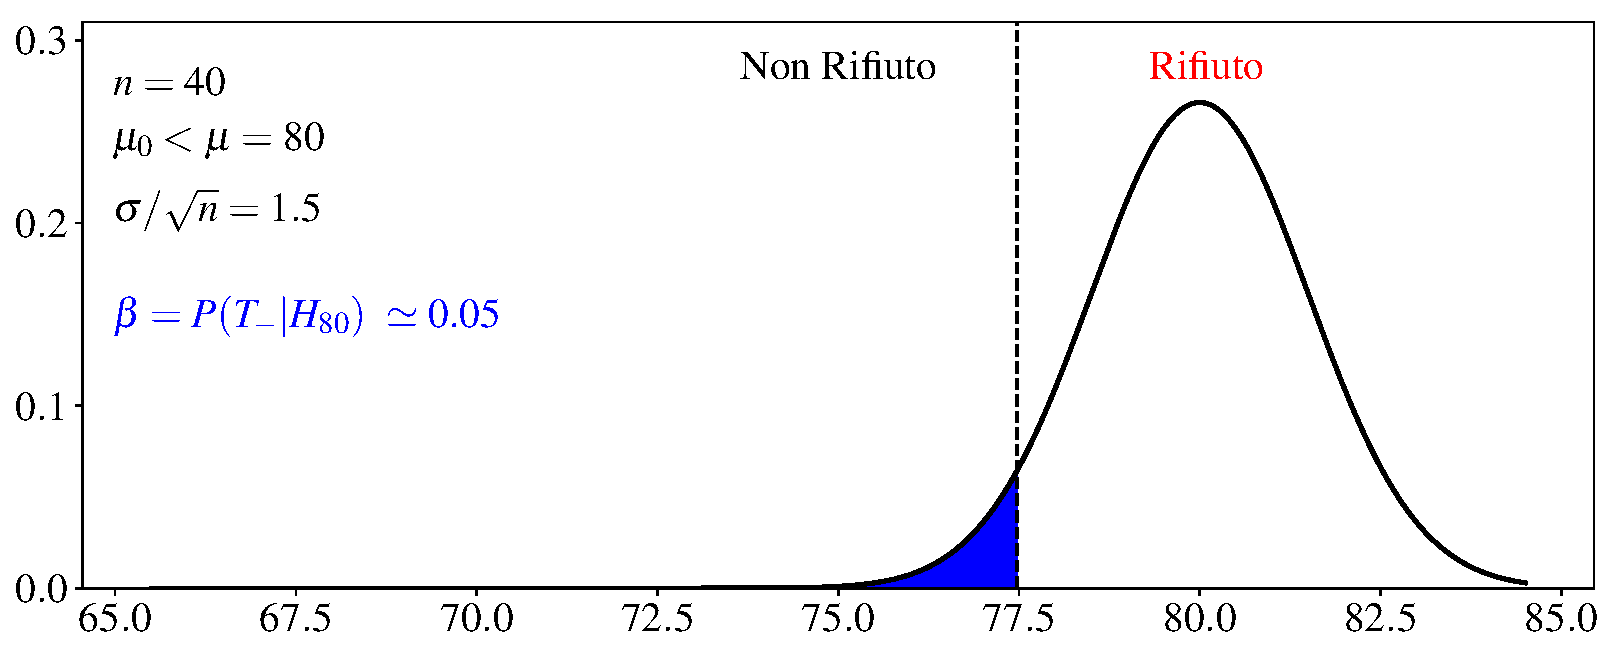
\includegraphics[width=0.8\textwidth]{figure/Z-test_04.pdf}



%%%%%%%%%%%%
%%%%%%%%%%%%
%%%%%%%%%%%%
\clearpage\subsection{Pressione diastolica (esercizio formato esame)}
\label{Pressione diastolica esercizio 1}

(Testo ripetuto da sopra~\ref{Z-test}.) Si sospetta che una certa terapia faccia aumentare la pressione diastolica. Nella popolazione generale la pressione diastolica ha distribuzione $N(\mu_0,\sigma^2)$ con $\mu_0=75$ e $\sigma=5.5$. Assumiamo che tra i pazienti in terapia la pressione diastolica sia distribuita normalmente con media ignota $\mu$ e con la stessa deviazione standard della popolazione generale. 

Un esperimento consiste nel misurare il valor medio della pressione diastolica di un campione di $n=64$ pazienti in terapia.

\textbf{Domande}

\begin{itemize}
\item[1.] Qual è l'ipotesi nulla?
\item[2.] Qual è l'ipotesi alternativa?
\item[3.] Quale test dobbiamo usare?
\item[4.] Qual è il valore di soglia $x_\alpha$ per rifiutare l'ipotesi nulla con una confidenza del $95\%$ (ovvero significatività del $5\%$)~?
\item[5.] Dato il valore di soglia al punto precedente, qual è la potenza del test per un effect size $\delta=2$~? 
\end{itemize}
Si risponda assumendo note le funzioni in calce.

\textbf{Risposte}\  Definiamo\ $\mu_0=75$,\quad $\sigma=5.5$,\quad, $n=64$,\quad $\delta=2$. Sia $Y$ la v.a. che da il valor medio della pressione diastolica del campione.

\begin{itemize}
\item[1.] $H_0$: $\mu=\mu_0$ dove $\mu$ è pressione diastolica delle persone in terapia 
\item[2.] $H_A$: $\mu>\mu_0$
\item[3.] Z-test a una coda (coda superiore)
\item[4.] $x_\alpha$ è tale che \medskip

$\alpha\ =\ \Pr\big(Y\ge x_\alpha\ \mathbin\big|\ \mu=\mu_0\big)\ =\ \Pr(X\ge x_\alpha)$, dove $X\sim N(\mu_0,\sigma^2/n)$ \medskip

$\phantom{\alpha\ }\ =1-\Pr\bigg(Z\le \dfrac{x_\alpha-\mu_0}{\sigma/\sqrt n}\bigg)$, dove $Z\sim N(0,1)$.

\hfill $x_\alpha\ =\ \dfrac{\sigma}{\sqrt n}\,{\tt qnorm}(1-\alpha)-\mu_0$.

\item[5.] La potenza del test è $1-\beta$ dove\medskip

$\beta\ =\ \Pr(Y\le x_\alpha\ |\ \mu=\mu_0+\delta)\ =\ \Pr(X\le x_\alpha)$, dove $\bar X\sim N(\mu_0+\delta,\sigma^2/n)$\medskip


$\phantom{\beta\ }=\ \Pr\bigg(Z\le  \dfrac{x_\alpha-\mu_0-\delta}{\sigma/\sqrt n}\bigg)$

\hfill$\beta\ =\  {\tt pnorm}\bigg(\dfrac{x_\alpha-\mu_0-\delta}{\sigma/\sqrt n}\bigg)$

\end{itemize}

\vfill
\parskip1ex
{\hrulefill\scriptsize

{\tt pbinom(x,n,p)}=$P(X\le x)$, per $X\sim B(n,p)$
\hfill 
{\tt qbinom($\alpha$,n,p)=x},  dove $P(X\le x)=\alpha$ per $X\sim B(n,p)$

{\tt pnorm(z)}=$P(Z\le z)$, per $Z\sim N(0,1)$
\hfill 
{\tt qnorm($\alpha$)=z},  dove $P(Z\le z)=\alpha$ per $Z\sim N(0,1)$

{\tt pt(t,$\nu$)} = $P(T\le t)$ per $T\sim t(\nu)$
\hfill
{\tt qt($\alpha$,$\nu$)=t}, dove $P(T\le t)=\alpha$ per $T\sim t(\nu)$

{\tt pchisq(q,k)} = $P(Q\le q)$, per $Q\sim \chi^2_k$
\hfill
{\tt qchisq($\alpha$,k)=q},  dove $P(Q\le q)=\alpha$ per $Q\sim \chi^2_k$
\par
}


\begin{comment}
%%%%%%%%%%%%
%%%%%%%%%%%%
%%%%%%%%%%%%
\clearpage\
\subsection{Prevalenza mancinismo 3 (domanda in formato esame)}
\label{mancini3}
\hfill\textbf{{\color{brown}\hyperref[CLT]{Il teorema del limite centrale \faShare}}}

Il $10\%$ è delle persone sono mancine. Ci chiediamo se la caratteristica sia ereditaria. Eseguiamo il seguente esperimento. Selezioniamo un campione di $1000$ persone con almeno un genitore mancino e misuriamo la frequenza di mancini.

\textbf{Domande}

\begin{itemize}
\item[1.] Qual è l'potesi nulla?

\item[2.] Qual è l'potesi alternativa?

\item[3.] Che test possiamo fare?

\item[4.] Quale valore di soglia otteniamo se vogliamo rifiutare $H_0$ con una significatività del $5\%$~?
\end{itemize}

\textbf{Risposte} \ Definiamo: 
$p_0=10\%$\\
$p=$  prevalenza del mancinismo tra i figli di genitori mancini\\
$\sigma_0=\sqrt{n\, p_0(1-p_0)}$\\
$n=1000$\\
$x = $ frequenza relativa rilevata\\
$z=\dfrac{x - p_0}{\sigma_0/\sqrt{n}}=\dfrac{x - p_0}{\sqrt{p_0(1-p_0)}}$\\

\begin{itemize}
\item[1.] $H_0$: \ $p=p_0$ 
\item[2.] $H_A$: \ $p>p_0$ 
\item[3.] Z-test a una coda (superiore). Approssimiamo binomiale con normale.
\item[4.] La soglia per $z$ è $z_\alpha$ tale che $\alpha=\Pr(Z>z_\alpha)$. Quindi $z_\alpha\ =\ ${\tt qnorm(1-$\alpha$)}\\
La soglia per la frequenza è $x_\alpha\ =\ z_\alpha\sqrt{p_0(1-p_0)} +p_0$.
\end{itemize}

\textit{N.B. avremmo potuto usare il test binomiale.}

\parskip1ex
{\hrulefill\scriptsize

Si assumano noti i valori delle seguenti funzioni

{\tt pbinom(x,n,p)}=$P(X\le x)$, per $X\sim B(n,p)$
\hfill 
{\tt qbinom($\alpha$,n,p)=x},  dove $P(X\le x)=\alpha$ per $X\sim B(n,p)$

{\tt pnorm(z)}=$P(Z\le z)$, per $Z\sim N(0,1)$
\hfill 
{\tt qnorm($\alpha$)=z},  dove $P(Z\le z)=\alpha$ per $Z\sim N(0,1)$

{\tt pt(t,$\nu$)} = $P(T\le t)$ per $T\sim t(\nu)$
\hfill
{\tt qt($\alpha$,$\nu$)=t}, dove $P(T\le t)=\alpha$ per $T\sim t(\nu)$

{\tt pchisq(q,k)} = $P(Q\le q)$, per $Q\sim \chi^2_k$
\hfill
{\tt qchisq($\alpha$,k)=q},  dove $P(Q\le q)=\alpha$ per $Q\sim \chi^2_k$
\par
}
  
\end{comment}



%%%%%%%%%%%%
%%%%%%%%%%%%
%%%%%%%%%%%%
\clearpage
\hfill\textbf{{\color{brown}\hyperref[pvalore]{Il p-valore \faShare}}}
\subsection{Una coda, p-valore}
(Continua l'esempio~\ref{Z-test}.) Supponiamo di ottenere $\bar x=78.0$ da un campione di dimensione $n=20$. Il p-valore di questa misura è $\Pr(\bar X\ge 78)=1-\Pr(\bar X\le 78)$.

\hfil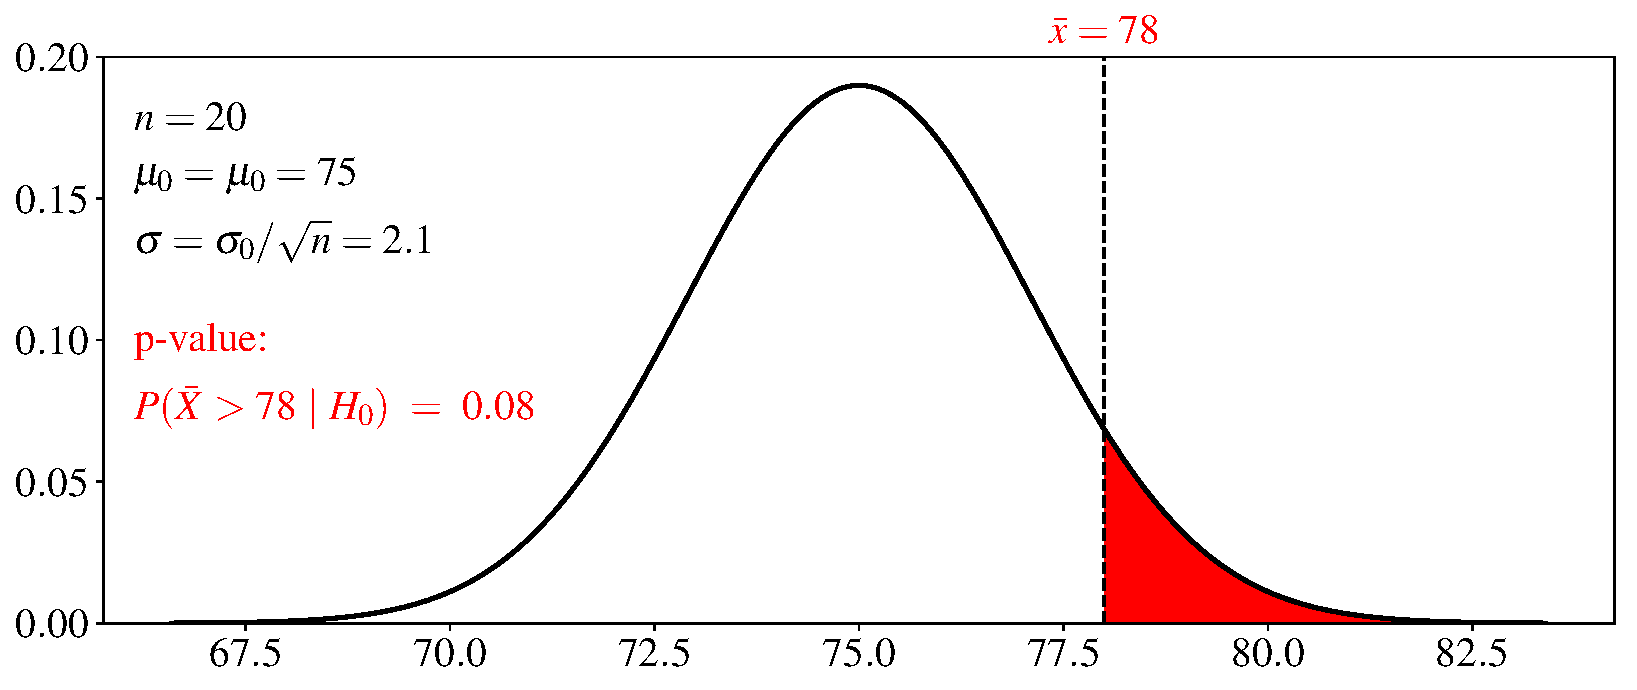
\includegraphics[width=0.8\textwidth]{figure/Z-test-p-val_01.pdf}

Numericamente $\Pr(\bar X\le \bar x)$ si può calcolare usando la funzione {\tt pnorm(x,m,s)} Nel nostro caso i valori sono \ {\tt x}$\,=\bar x$,  \ {\tt m}$\,=\mu_0$, \ e  \ {\tt s}$\,=\sigma/\sqrt{n}$

Nel caso di un test a due code, se $H_A$ fosse stata $\mu_0\neq\mu$, il p-valore diventa esattamente il doppio che per il test ad una coda (qui sotto differisce numericamente a causa degli arrotondamenti). 

\hfil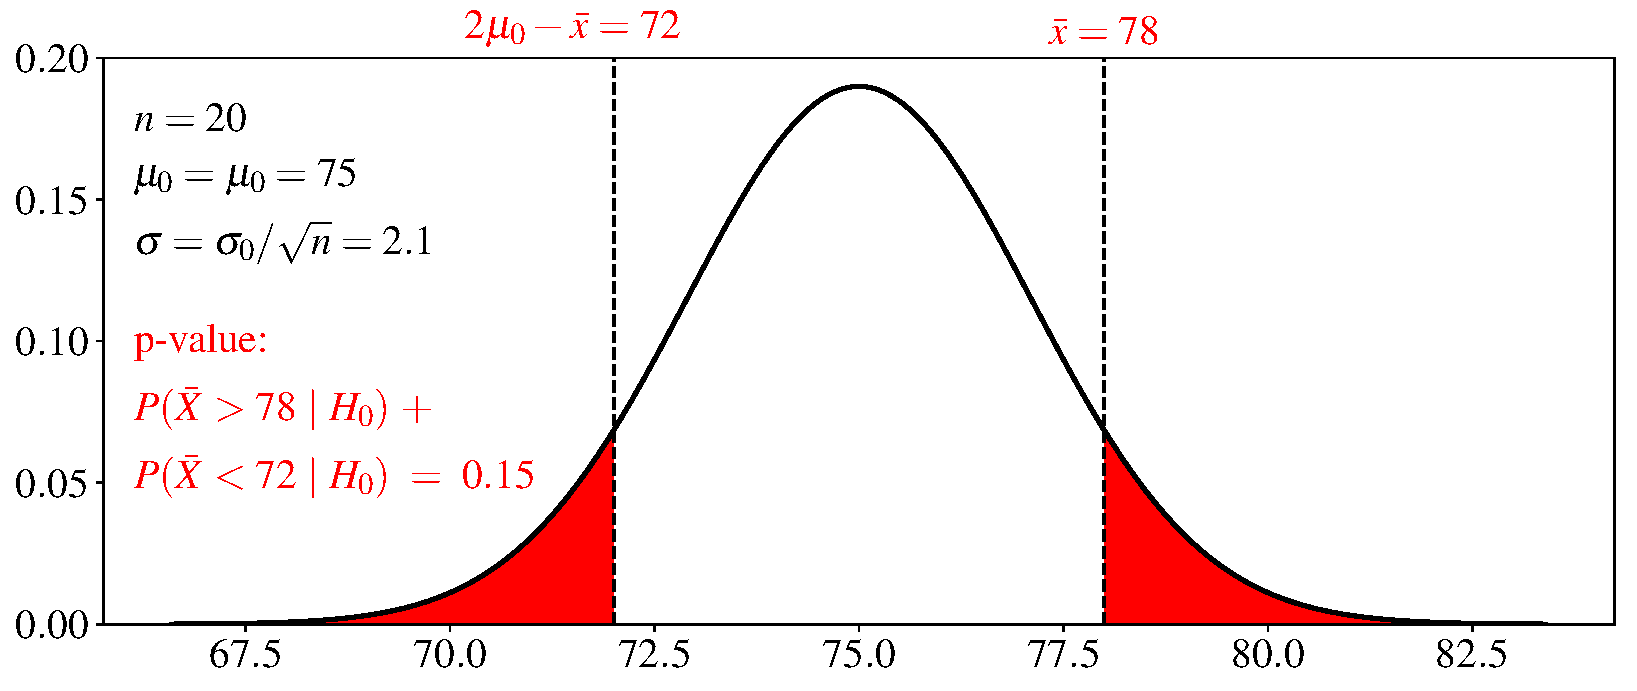
\includegraphics[width=0.8\textwidth]{figure/Z-test-p-val_02.pdf}


%%%%%%%%%%%%
%%%%%%%%%%%%
%%%%%%%%%%%%
\clearpage\subsection{Pressione diastolica cont. (esercizio formato esame)}
\label{Pressione diastolica esercizio 2}

Continua da~\ref{Pressione diastolica esercizio 1}

\textbf{Domande}

\begin{itemize}
\item[6.] Supponiamo che il valore medio della pressione diastolica nel nostro campione sia $78$. 
Con che p-valore possiamo rifiutare l'ipotesi nulla?
\end{itemize}
Si risponda assumendo note le funzioni in calce.

\textbf{Risposte}\  Definiamo\ $\bar x=78$.\medskip

\begin{itemize}
\item[6.] 

p-valore$\ =\ \Pr\big(Y\ge \bar x\ \mathbin\big|\ \mu=\mu_0\big)\ =\ \Pr(X\ge\bar x)$, dove $X\sim N(\mu_0,\sigma^2/n)$\medskip\smallskip

\phantom{p-valore}$\ =\ 1-\Pr\bigg(Z\le \dfrac{\bar x-\mu_0}{\sigma/\sqrt n}\bigg)$, dove $Z\sim N(0,1)$\medskip

\phantom{p-valore}$\ =\ 1- {\tt pnorm}\bigg(\dfrac{\bar x-\mu_0}{\sigma/\sqrt n}\bigg)$.

\end{itemize}

\vfill
\parskip1ex
{\hrulefill\scriptsize

{\tt pbinom(x,n,p)}=$P(X\le x)$, per $X\sim B(n,p)$
\hfill 
{\tt qbinom($\alpha$,n,p)=x},  dove $P(X\le x)=\alpha$ per $X\sim B(n,p)$

{\tt pnorm(z)}=$P(Z\le z)$, per $Z\sim N(0,1)$
\hfill 
{\tt qnorm($\alpha$)=z},  dove $P(Z\le z)=\alpha$ per $Z\sim N(0,1)$

{\tt pt(t,$\nu$)} = $P(T\le t)$ per $T\sim t(\nu)$
\hfill
{\tt qt($\alpha$,$\nu$)=t}, dove $P(T\le t)=\alpha$ per $T\sim t(\nu)$

{\tt pchisq(q,k)} = $P(Q\le q)$, per $Q\sim \chi^2_k$
\hfill
{\tt qchisq($\alpha$,k)=q},  dove $P(Q\le q)=\alpha$ per $Q\sim \chi^2_k$
\par
}

%%%%%%%%%%%%
%%%%%%%%%%%%
%%%%%%%%%%%%
\clearpage\subsection{Crescita media}

In condizioni ottimali l'incremento di una certa cultura in una fissata unità di tempo ha media $\mu_0=3.1$ e deviazione standard $\sigma=1.2$. Vogliamo progettare un test per decidere se la crecita di una data cultura sia sub-ottimale. Assumiamo che la distribuzione sia normale e che in condizioni sub-ottimali la deviazione standard sia la stessa. (Queste assunzioni sono abbastanza irragionevoli, ma portiamo pazienza.)

Domande:

\begin{itemize}
\item[1] Preleviamo $n=9$ campioni, e misuriamo la crescita in un'unità di tempo. E calcoliamo la media campionaria $\bar x$. Quanto dev'essere $x_\alpha$ per poter affermare che con significatività $\alpha=1\%$ che siamo in condizioni sub-ottimali quando $\bar x<x_\alpha$~?
\item[2] Dato $x_\alpha$ come sopra. Qual'è la probabilità di un errore del II tipo se l'effect size è $\delta=0.5$~?
\end{itemize}

Risposte:

\begin{itemize}
\item[1] Vogliamo $1\%=\Pr(\bar X\le x_\alpha)$ con $\bar X\sim N(\mu_0,\sigma/\sqrt{n})$.\\
Quindi $x_\alpha=${\tt\ qnorm(0.01,3.1,0.4)\,=\,2.17}
\item[2] $\beta=\Pr(\bar X\le x_\alpha)$ con $\bar X\sim N(\mu_0-\delta,\sigma/\sqrt{n})$.\\
Quindi  $\beta=${\tt\ pnorm(2.17,2.6,0.4)\,=\,0.14}.

\end{itemize}



%%%%%%%%%%%%
%%%%%%%%%%%%
%%%%%%%%%%%%
\clearpage\
\subsection{Mean weight (domanda in formato esame)}

Boys of a certain age are known to have a mean weight of $85$ pounds and standard deviation $10.6$ pounds. A complaint is made that the boys living in a municipal children's home are overfed. As one bit of evidence, $25$ boys (of the same age) are weighed and found to have a mean weight of $88.94$ pounds. Assume the same standard deviation as in the general the population (the unrealistic part of this example).


\textbf{Domande}

\begin{itemize}
\item[1.] Qual è l'potesi nulla?

\item[2.] Qual è l'potesi alternativa?

\item[3.] Che test possiamo fare?

\item[4.] Qual'è il p-valore ottenuto dai dati?

\item[5.] Possiamo rigettare l'ipotesi nulla con una significatività del $\alpha=5\%$~?
\end{itemize}

\textbf{Risposte} Definiamo:\\
$\mu_0=85$\\
$\sigma=10.6$\\
$n=25$\\
$\bar x=88.94$
\begin{itemize}
\item[1.] $\mu=\mu_0$.
\item[2.] $\mu>\mu_0$ 
\item[3.] Z-test una coda (superiore)
\item[4.] il p-valore è {\tt 1-pnorm(z)} dove $z=\dfrac{\bar x-\mu_0}{\sigma/\sqrt{n}}$.\hfill {\tt (0.03)}

Lo stesso risultato si ottienre con {\tt 1-pnorm($\bar x,\mu_0,\sigma/\sqrt{n}$)}, ma non è tra le possibilità elencate in calce.
\item[5.] si, perché  p-valore $<\alpha$.
\end{itemize}

\parskip1ex
{\hrulefill\scriptsize

Si assumano noti i valori delle seguenti funzioni

{\tt pbinom(x,n,p)}=$P(X\le x)$, per $X\sim B(n,p)$
\hfill 
{\tt qbinom($\alpha$,n,p)=x},  dove $P(X\le x)=\alpha$ per $X\sim B(n,p)$

{\tt pnorm(z)}=$P(Z\le z)$, per $Z\sim N(0,1)$
\hfill 
{\tt qnorm($\alpha$)=z},  dove $P(Z\le z)=\alpha$ per $Z\sim N(0,1)$

{\tt pt(t,$\nu$)} = $P(T\le t)$ per $T\sim t(\nu)$
\hfill
{\tt qt($\alpha$,$\nu$)=t}, dove $P(T\le t)=\alpha$ per $T\sim t(\nu)$

{\tt pchisq(q,k)} = $P(Q\le q)$, per $Q\sim \chi^2_k$
\hfill
{\tt qchisq($\alpha$,k)=q},  dove $P(Q\le q)=\alpha$ per $Q\sim \chi^2_k$
\par
}



%%%%%%%%%%%%
%%%%%%%%%%%%
%%%%%%%%%%%%
\clearpage\ 
\hfill\textbf{{\color{brown}\hyperref[tStudent]{La distribuzione t di Student \faShare}}}
\section{T-test}
\label{T-test}
\subsection{Una popolazione}
A professor wants to know if her introductory statistics class has a good grasp of basic math. Six students are chosen at random from the class and given a math proficiency test. The professor wants the class to be able to score above 70 on the test. The six students get scores of 62, 92, 75, 68, 83, and 95. Can the professor have 90\%  confidence that the mean score for the class on the test would be above 70?

$\strut n=6$

$\mu_0=70$

$\bar x =\dfrac1n\big(62+92+75+68+83+95\big) =79.17$

$s = \sqrt{\dfrac{\strut(62-\bar x)^2+(92-\bar x)^2+(75-\bar x)^2+(68-\bar x)^2+(83-\bar x)^2+(95-\bar x)^2}{n-1}}$

$\strut\phantom{s} = 13.17$

\begin{itemize}
\item[1.] $H_0$ \ $\mu_0 = 70$

\item[2.] $H_A$ \ $\mu>\mu_0$

\item[3.] $T$-test due popolazioni (dati non accoppiati) coda superiore. 

\item[4.] Il $t$-score è 
$t = \dfrac{\bar x - \mu_0}{s/\sqrt{n}}=\dfrac{79.17-70}{13.17/\sqrt{6}} = 1.71$

\item[5.] Il p-valore è $\Pr(T\ge t)$ dve $T\sim t(5)$. Ovvero {\tt pt($t$, $n-1$)}\hfill{\tt (0.074)}

\vfill
\hrulefill\hfill\hfill

In R la funzione il risultato si ottiene direttamente con

{\tt 
x = c(62,92,75,68,83,95)\\
t.test(x, alternative='greater', mu=70)}

Quindi possiamo affermare con un livello di confidenza $\ge 90\%$ che il voto medio della classe in un ipotetico esame sarà del $>70$.  
\end{itemize}


%%%%%%%%%%%%
%%%%%%%%%%%%
%%%%%%%%%%%%
\clearpage\
\subsection{Due popolazioni}
Si sospetta che un certo medicinale modifichi la pressione diastolica.  Prendiamo due gruppi di $n_x=6$ e $n_y=5$ persone. Al primo gruppo somministriamo il medicinale al secondo un placebo. Assumiamo che in entrambi i casi la pressione diastolica sia distribuita normalmente con la stessa deviazione standard (ignota). Nel primo gruppo otteniamo i valori $x_1,\dots,x_6=62,92,75,68,83,95$ nel secondo gruppo $y_1,\dots,y_5=60,95,76,69,89$.

\begin{itemize}
\item[1.] $H_0$ \ $\mu_x = \mu_y$\hfill la media nelle due popolazioni è la stessa 

\item[2.] $H_A$ \ $\mu_x\neq\mu_y$\hfill la media nelle due popolazioni è diversa 


\item[3.] $T$-test a due code per due popolazioni con dati accoppiati

\item[3.] Il $t$-score è 
$t = \dfrac{\bar x - \bar y}{\sqrt{s^2_x/n_x+s^2_y/n_y}}$ dove 

$\displaystyle\bar x = \frac1{n_x}\sum^{n_x}_{i=1}x_i$\hfil$\displaystyle\bar y = \frac1{n_y}\sum^{n_y}_{i=1}y_i$


$\displaystyle s^2_x= \frac1{n_x-1}\sum^{n_x}_{i=1}(x_i-\bar x)^2$\hfil
$\displaystyle s^2_y= \frac1{n_y-1}\sum^{n_y}_{i=1}(y_i-\bar y)^2$




\item[4.] Il p-valore è $2\Pr(T\ge |t|)$ dove $T\sim t(n_x+n_y-2)$.\\ 
Ovvero {\tt 2 * (1 - pt($|t|$, $n_x+n_y-2$))}

\hrulefill\hfill\hfill

In R la funzione il risultato si ottiene direttamente con

{\tt 
x = c(62,92,75,68,83,95)\\
y = c(60,95,76,69,89)\\
t.test(x, y, alternative='two', var.equal = TRUE)}
\end{itemize}

%%%%%%%%%%%%
%%%%%%%%%%%%
%%%%%%%%%%%%
\clearpage\
\subsection{Dati accoppiati}

Si sospetta che un certo medicinale modifichi la pressione diastolica.  Prendiamo un gruppo di $n=6$ persone. Somministriamo ad ogni individuo prima un placebo e successivamente il medicinale. Assumiamo che in entrambi i casi la pressione diastolica sia distribuita normalmente. Con il placebo otteniamo i valori $x_1,\dots,x_6=62,92,75,68,83,95$ con il medicinale otteniamo i valori $y_1,\dots,y_6=60,95,76,69,89,90$.



\begin{itemize}
\item[1.] $H_0$ \ $\mu = 0$\hfill la media delle differenze è $0$

\item[2.] $H_A$ \ $\mu\neq0$

\item[3.] $T$-test per due campioni accoppiati a due code

\item[3.] Il $t$-score è 
$t = \dfrac{\bar z}{s/\sqrt{n}}$ dove $z_i=x_i-y_i$ e

$\displaystyle\bar z = \frac1{n}\sum^n_{i=1}z_i$

$\displaystyle s^2= \frac1{n-1}\sum^n_{i=1}(z_i-\bar z)^2$

\item[4.] Il p-valore è $2\Pr(T\ge |t|)$ dove $T\sim t(n-1)$.\\ 
Ovvero {\tt 2 * (1 - pt($|t|$, $n-1$))}

\hrulefill\hfill\hfill

In R la funzione il risultato si ottiene direttamente con

{\tt 
x = c(62,92,75,68,83,95)\\
y = c(60,95,76,69,89,90)\\
t.test(x, y, alternative='two', paired=TRUE)}
\end{itemize}



%%%%%%%%%%%%
%%%%%%%%%%%%
%%%%%%%%%%%%
\clearpage\
\section{Intervallo di confidenza}
\label{ICTesempio1}
\hfill\textbf{{\color{brown}\hyperref[IC_varianza_ignota]{Intervallo di confidenza: normale con varianza ignota \faShare}}}


\hfill\textbf{{\color{brown}\hyperref[IC_varianza_nota]{varianza nota \faShare}}}

Da una popolazione con distribuzione normale, media e varianza ignota, misuriamo i valori $x_1,\dots,x_6=62,92,75,68,83,95$. Si calcoli un intervallo di confidenza al $95\%$ per la media di popolazione.

\ceq{\hfill\bar x}{=}{ \frac1{6}\sum^6_{i=1}x_i}\hfill {\tt (79.17)}

\ceq{\hfill s}{=}{ \sqrt{\frac1{5}\sum^{6}_{i=1}(x_i-\bar x)^2}}\hfill {\tt (13.17)}

L'intervallo di confidenza è $\bar x\pm\epsilon$ dove $\epsilon$ è tale che 

\ceq{\hfill 0.95}{=}{\Pr\bigg(-\frac{\epsilon}{s/\sqrt{n}}<T<\frac{\epsilon}{s/\sqrt{n}}\bigg)}

Sia $t\ =\ ${\tt -qt(0.025,5) $\simeq$ 2.57} allora 

\ceq{\hfill\epsilon}{=}{\dfrac{t\,s}{\sqrt{6}}}\hfill {\tt (13.82)}

N.B. Se la deviazione standard della popolazione fosse stata nota, diciamo $\sigma=13.17$ allora posto $z\ =\ ${\tt -qnorm(0.25) $\simeq$ 0.67} avremmo ottenuto

\ceq{\hfill\epsilon}{=}{\dfrac{z\,\sigma}{\sqrt{6}}}\hfill {\tt (16.35)}


%%%%%%%%%%%%
%%%%%%%%%%%%
%%%%%%%%%%%%
%%%%%%\clearpage\section{Esercizi vari}
\subsection{Placebo}


Ad un gruppo di persone vengono misurati 100 diversi parametri fisiologici (che assumiamo indipendenti) prima e dopo l'assunzione di un placebo. Per ognuno di questi parametri l'ipotesi nulla è che non ci sia differenza. Supponendo che il placebo non causi alcuna differenza, qual'è la probabilità che per almeno uno di questi parametri si ottenga p-valore $<0.02$~?


Risposta:\kern3ex $1-(0.98)^{100}=87\%$

\clearpage\
\begin{comment}
\section{Inferenza Bayesiana}

In un casinó si gioca a testa o croce ($1$ o $0$) con tre tipi di monete che hanno probabilità di successo $1/2$, $2/3$, e $1/3$. Il casinò sceglie la moneta e continua a giocare con la stessa moneta per tutto il giorno. Il giocatore non sa quale moneta sia scelta.

Assumiamo per fissare le idee che il casinò scelga la monete a sorte e che le tre monete abbiano la stessa probabilità di essere scelte. Supponiamo osservare la sequenza $010$ e di voler puntare sul prossimo lancio. Ci interessa sapere con che probabilità possiamo assumere quale moneta.  

Siano $M_{1/2}$, $M_{2/3}$ ed $M_{1/3}$ gli eventi che corrispondono alla scelta delle tre monete
$M_{1/2}$, $M_{2/3}$ ed $M_{1/3}$

$\Pr(010\mathrel|M_{1/2})\ =\ \dfrac{1}{2^3}\ =\ \dfrac{1}{8}$

$\Pr(010\mathrel|M_{2/3})\ =\ \dfrac{1}{3}\cdot\dfrac{2}{3}\cdot\dfrac{1}{3}\ =\ \dfrac{2}{9}$

$\Pr(010\mathrel|M_{1/3})\ =\ \dfrac{2}{3}\cdot\dfrac{1}{3}\cdot\dfrac{2}{3}\ =\ \dfrac{4}{9}$

\smallskip
Usando il teorema delle probabilità totali possiamo facilmente calcolare 

$\Pr(010)\ =\ \dfrac{1}{3}\left(\dfrac{1}{8}+\dfrac{2}{9}+\dfrac{4}{9}\right)\ =\ \dfrac{19}{72}$.

Quindi possiamo calcolare la probabilità di $M_{1/2}$, $M_{2/3}$ ed $M_{1/3}$ data l'informazione $010$.

$\Pr(M_{1/2} \mathrel| 010)=\dfrac{\Pr(010\mathrel|M_{1/2})\cdot \Pr(M_{1/2})}{\Pr(010)}=\dfrac{1/8\cdot 1/3}{19/72}$

$\Pr(M_{2/3} \mathrel| 010)=\dfrac{\Pr(010\mathrel|M_{2/3})\cdot \Pr(M_{2/3})}{\Pr(010)}=\dfrac{2/9\cdot 1/3}{19/72}$

$\Pr(M_{1/3} \mathrel| 010)=\dfrac{\Pr(010\mathrel|M_{1/3})\cdot \Pr(M_{1/3})}{\Pr(010)}=\dfrac{4/9\cdot 1/3}{19/72}$


\chapter{Appendice}

\section{Il simbolo di sommatoria}

Data una sequenza finita $(a_i\ :\ i=0,\dots,n)$ scriveremo.

\ceq{\hfill\sum^n_{i=0} a_i}{=}{a_0+a_1+\dots+a_n}

\par\medskip
Propriet\`a importanti:

\ceq{\hfill\sum^n_{i=0} c\cdot a_i}{=}{c\cdot\sum^n_{i=0} a_i}\hfill dove $c$ \`e una costante arbitraria.

\ceq{\hfill\sum^n_{i=0} (a_i+b_i)}{=}{ \bigg(\sum^n_{i=0} a_i\bigg) +\bigg(\sum^n_{i=0} b_i\bigg).}

\ceq{\hfill\sum^n_{i=0} 1}{=}{n.}


\clearpage\section{Esercizi}

Verificare le seguenti identit\`a 

\ceq{\hfill\sum^{n-1}_{i=0} a_i}{=}{\sum^{n}_{i=1} a_{i-1}}

\ceq{\hfill\sum^{n}_{i=0} a_i}{=}{a_0+\sum^{n}_{i=1} a_i}

\ceq{\hfill\sum^{2n}_{i=1} a_i}{=}{\sum^n_{i=1} a_i +\sum^{2n}_{i=n+1} a_i}

\ceq{}{=}{\sum^n_{i=1} a_{2i} +\sum^{n-1}_{i=0} a_{2i+1}}

\ceq{}{=}{\sum^n_{i=1} a_{2i} +\sum^{n}_{i=1} a_{2i-1}.}


\clearpage\section{Sommatorie "disordinate"}
\label{sommatorie_disordinate}

Sia $D$ un insieme finito, diciamo $D\subseteq\{0,\dots,n\}$.

Sia $(a_i\ :\ i=0,\dots,n)$ una sequenza finita definiamo

\ceq{\hfill\sum_{i\in D} a_i}{=}{a_{i_0}+\dots+a_{i_k}}\hfill dove $D=\{i_0,\dots,i_k\}$.

Per esempio possiamo scrivere


\ceq{\hfill\sum^n_{i=0} a_i}{=}{\sum_{i\in P_n} a_i+\sum_{i\in D_n} a_i}

dove $P_n=\big\{0\le i\le n : i\ \textrm{pari}\big\}$\quad
e 
\quad$D_n=\big\{0\le i\le n : i\ \textrm{dispari}\big\}$.

La stessa notazione può essere usata senza ambiguità anche quando $D$ è un insieme finito non necessariamente numerico (né ordinabile in alcun modo). Per esempio, 

$D=\{{\rm rosso, giallo, blu}\}$,\hfil $a_{{\rm rosso}}=2$,\hfil $a_{{\rm giallo}}=1$,\hfil $a_{{\rm blu}}=6$,

\ceq{\hfill\sum_{i\in D} a_i}{=}{9}.



\clearpage\section{Sommatorie su due indici}

Sia $a:D\to \RR$ una mappa con dominio finito  $D=\{0,\dots,n\}^2$.

Indicheremo $a$ con $(a_{i,j}: 0\le i,j\le n)$ o notazione simile.

Possiamo immaginare $(a_{i,j})_{0\le i,j\le n}$ come una matrice

\hspace*{20ex}
$\displaystyle\begin{array}{cccc}
a_{0,0}&a_{0,1}&\dots&a_{0,n}\\[1ex]
a_{1,0}&a_{1,1}&\dots&a_{1,n}\\[2ex]
\vdots&\vdots&&\vdots\\[2ex]
a_{n,0}&a_{n,1}&\dots&a_{n,n}\\
\end{array}$

\hfil$\displaystyle\sum^n_{i,j=0} a_{i,j}\quad =\quad$ somma di tutti gli elementi della matrice


Per l'associativit\`a della somma possiamo riscrivere la somma

\parbox{20ex}{\hfill$\displaystyle\sum^n_{i,j=0} a_{i,j}$}$\displaystyle\quad =\quad\sum^n_{i=0}\sum^n_{j=0}a_{i,j}$


$\displaystyle\begin{array}{ccccccccc}
\displaystyle\sum^n_{j=0}a_{0,j}&=& a_{0,0}&+&a_{0,1}&+&\dots&+&a_{0,n}\\[1ex]
\displaystyle\sum^n_{j=0}a_{1,j}&=& a_{1,0}&+&a_{1,1}&+&\dots&+&a_{1,n}\\[2ex]
\vdots\\[2ex]
\displaystyle\sum^n_{j=0}a_{n,j}&=& a_{n,0}&+&a_{n,1}&+&\dots&+&a_{n,n}\\
\end{array}$

\end{comment}
\end{document}
